\chapter{Introduction}\label{sec:introductionux5fchapter}

Large-scale (global) models of the atmosphere and climate system are
fundamental tools that aid in our understanding of climate system. They
are used not only to study interactions between different components of
the climate system, but also to perform simulations of future climate
change relevant for informing government policy decisions. The
formulation of these models are evaluated on multiple scales, from
testing the individual components that go into the models (such as a
particular physical process like convection) to evaluating the
simulation of climate as a whole. On the large-scale, models are often
evaluated by comparing simulations of present-day climate with
observations of the present-day climate system. The sources for these
observations are diverse, and depend on the particular aspect of the
climate being evaluated.

Clouds are a critic piece of the climate system, and yet the simulation
of clouds by global climate models (GCMs, also general circulation
models) remains a challenge, and cloud feedback processes are well-known
to be a primary source of uncertainty in projections of future climate
(Cess et al. 1990; Bony and Dufresne 2005; Williams and Webb 2009;
Medeiros et al. 2008; Dufresne and Bony 2008; Bony et al. 2006). This
makes evaluation of clouds in large-scale models of utmost importance.

Observational records of cloud occurrence and other properties from
satellite imagers including the International Satellite Cloud
Climatology Project (ISCCP Rossow and Schiffer 1999), the Moderate
Resolution Imaging Spectroradiometer (MODIS King et al. 2003), and the
Multi-angle Imaging Spectroradiometer (MISR Diner et al. 2002; Diner et
al. 2005) provide a natural baseline for the evaluation of the
large-scale cloud statistics simulated by these models because they
provide near-global coverage and an increasingly long time-series.
Comparisons of this type have been used to evaluate models for as long
as such observations have been available {[}citations{]}, but
comparisons between satellite-retrieved and modeled cloud properties are
difficult because of fundamental differences between how clouds can be
measured from space and how they are represented in large-scale models.
These differences stem from both unavoidable limitations in the
satellite retrieval process, as well as from limitations that arise due
to the differences in scale between satellite retrievals and current
GCMs. For example, cloud top height or cloud top pressure retrievals
based on visible or infrared observations (e.g., ISCCP, MODIS, and MISR)
are known to have significant problems when clouds with low amounts of
condensate (i.e.~non-opaque clouds or cloud-tops) are present,
especially for scenes with multi-layer clouds where the upper layer
cloud is optically thin (Marchand et al. 2010; Pincus et al. 2012).
Fundamentally, the visible and infrared observations gathered by MODIS,
MISR and ISSCP cannot fully constrain the vertical distribution of
condensate, including discriminating between condensate types in
differing layers, and this leads to uncertainties and systematic errors
in the determination (retrieval) of cloud top height. Models, however,
specify (or resolve) the vertical distribution of condensate to some
degree. This fundamental difference between retrievals of cloud top
height and the vertical distribution of clouds specified by a model
makes any direct comparisons between the two somewhat ambiguous. An
alternative to this often ambiguous direct comparison between
satellite-retrieved and modeled clouds is to first ``simulate'' the
satellite view of clouds from the model-simulated atmospheric state. The
goal with this approach is to account for the known errors in the
satellite retrieval process by forward-modeling or emulating the
retrieval technique used for a particular satellite instrument from the
available model fields, with the goal of providing a description of what
a given satellite instrument would see given the model-simulated
atmosphere. These simulated or psuedo-retrievals are expected to be more
directly comparable to the available satellite retrievals than the raw
model fields, thus enabling a more appropriate evaluation of model
clouds against satellite observations.

The ISCCP simulator introduced by Klein and Jakob (1999) has been widely
used in model comparisons with ISCCP observations (Webb et al. 2001;
Norris and Weaver 2001; Lin and Zhang 2004; Zhang et al. 2005; Wyant et
al. 2006; Klein et al. 2013). The ISCCP simulator produces joint
histograms of cloud top pressure and cloud optical depth from model
fields that can be directly compared with joint histograms produced from
ISCCP retrievals. In effect, each bin in the ISCCP histogram is a cloud
fraction that quantifies how often clouds within a certain range of
cloud top pressures and cloud optical depths occur, and with the sum of
all bins yielding the total cloud fraction. Because outgoing longwave
radiation is strongly influenced by cloud top height (and cloud amount)
and outgoing shortwave radiation is strongly influenced by cloud optical
depth (and cloud amount), comparisons using the ISCCP joint histograms
provide an evaluation of model cloud amount that is linked to the impact
of clouds on the model radiation budget. This is extremely useful for
assigning radiative importance to diagnosed errors in cloud properties,
but is also useful for exploring cloud feedbacks associated with future
climate change. The latter point is demonstrated by M. D. Zelinka,
Klein, and Hartmann (2012a) and M. D. Zelinka, Klein, and Hartmann
(2012b), who exploit this link to the radiation budget to introduce a
new framework for calculating cloud feedbacks by creating a radiative
``kernel'' from the ISCCP histogram output by the ISCCP simulator that
represents the change in the radiative forcing that results from changes
in each of the ISCCP histogram components.

The utility of the ISCCP simulator has inspired efforts to construct
simulators for additional satellite-based imagers, including MISR
(Marchand and Ackerman 2010) and MODIS (Pincus et al. 2012). Additional
simulators have also recently been developed for the CloudSat (Stephens
et al. 2002) cloud profiling radar (Quickbeam; Haynes et al. 2007), and
for the Cloud-Aerosol Lidar with Orthogonal Polarization (CALIOP) lidar
(Chepfer et al. 2008) onboard the Cloud-Aerosol Lidar and Infrared
Pathfinder Satellite Observations (CALIPSO Winker, Hunt, and McGill
2007) satellite. {[}comment on evalations using the individual
simulators{]}

With the goal of facilitating the implementation of these simulators
into global climate models, the Cloud Feedback Model Intercomparison
Project (CFMIP; {[}citation{]}) has collected the ISCCP, MISR, MODIS,
CloudSat, and CALIPSO simulators into a single software package with a
common interface: the CMFIP Observation Simulator Package (COSP;
Bodas-Salcedo et al. 2011). This has enabled both coordinated
multi-model experiments comparing simulated cloud properties across
models as well as innovative multi-sensor analyses of models (e.g.,
Bodas-Salcedo et al. 2011; Kay et al. 2012; Klein et al. 2013),
nominally leading to more robust evaluation of clouds in climate models.

While the goal of the simulator approach is to remove ambiguities in
comparisons between models and remote sensing observations of clouds,
not all ambiguities in model-to-observation comparisons can be removed
with the simulator framework. The presence of remaining uncertainties or
ambiguities in simulated and retrieved cloud properties that are
unaccounted for or poorly represented by the simulators may undermine
conclusions reached using this framework. It is therefore important to
identify and understand the uncertainties and limitations of this
framework in order to be able to confidently attribute differences
between simulated and retrieved cloud properties unambiguously to model
biases.

As described by Pincus et al. (2012) and illustrated schematically by
Bodas-Salcedo et al. (2011) (see Figure 1 in Bodas-Salcedo et al.
(2011), and also Figure~\ref{fig:simulator_schematic} here), simulating
satellite retrievals from global model output is essentially a
three-part process, involving 1) inferring pixel-scale cloud properties
from the large-scale description provided by models, 2) simulating the
pixel-scale satellite retrievals from the inferred pixel-scale (or
subgrid-scale) cloud properties from the model, and finally 3)
aggregating the simulated pixel-scale retrievals into statistical
summaries consistent with the gridded, global summary products
distributed by the satellite teams (often referred to as ``Level 3''
products in satellite retrieval nomenclature). In general, there can be
errors associated with each of these three steps in the simulator
process, and the primary goal of the present study is to identify and
quantify these errors, and ultimately to present strategies for reducing
these errors in order to enable more robust evaluation of models in the
future.

\begin{figure}[htbp]
\centering
\includegraphics{graphics/simulator_schematic.pdf}
\caption{\label{fig:simulator_schematic}Schematic of the simulator
framework}\label{fig:simulatorux5fschematic}
\end{figure}

The first of these steps, inferring subgrid-scale cloud properties, is
necessary because the resolution of typical global models is much
coarser than the scales at which satellite retrievals are performed. As
pointed out by Pincus et al. (2012), these bulk statistics at the
gridbox scale imply a distribution of possible retrievals within each
gridbox, each resulting from a different possible combination of
subgrid-scale profiles. This is due to the fact that simple profiles of
averaged quantities at larger scales do not in themselves fully
constrain the distribution of profiles at smaller scales, and simulating
the satellite views of clouds depends on detailed knowledge of the
overlapping nature of clouds at scales approximating satellite pixels.
This is accounted for in the simulator framework by generating
stochastic samples of ``subcolumn'' profiles, which reproduce the
gridbox-averaged profiles in the limit of many samples and are
consistent with some external assumption about how the cloudy parts of
the gridbox overlap vertically (Klein and Jakob 1999). This problem is
not unique to simulating satellite-retrieved quantities, but is also
important for simulating radiative fluxes and heating rates within
models as well. However, the assumptions made in the subcolumn sampling
process, namely that cloud occurrence obeys a conceptually simple
combination of maximum and random overlap and that cloud (and
precipitation) condensate is horizontally homogeneous on the scale of
model gridboxes, have recently been shown to lead to substantial errors
in simulated radiative fluxes and heating rates in models (Barker,
Stephens, and Fu 1999; Oreopoulos et al. 2012) {[}others?{]}. In
Section~\ref{sec:subgrid1} here it is shown that these assumptions
similarly lead to substantial errors in simulated satellite retrievals.
In Section~\ref{sec:subgrid2} an improved framework for sampling these
subcolumns is presented that better represents the subgrid-scale cloud
and precipitation properties, and it is shown that these improvements
can substantially reduce the errors identified in
Section~\ref{sec:subgrid1}

Errors in the second step in the simulator framework (simulating the
pixel-scale satellite retrievals), can arise due to incomplete or
incorrect implementation of the retrieval process, even given perfect
pixel-scale cloud properties as inputs. While every effort is made to
build the simulators to account for as many features of the individual
retrievals as possible, verification of the simulators is difficult, and
documented verification is limited in the literature. The basic question
that largely remains unanswered is, given perfect descriptions of the
cloudy atmosphere as inputs to the simulators, are they able to
faithfully reproduce the retrieved cloud properties that the instrument
they attempt to simulate actually retrieves? A theoretical framework for
answering this question is to supply actual profiles of cloud properties
as inputs to the simulators, and then to compare the simulated
retrievals with actual coincident retrievals. Using this framework to
answer this question is difficult because it requires some source for
these ``perfect inputs'' on which to run the simulators simultaneous
with actual retrievals from the instruments. Mace et al. (2009) and Mace
et al. (2011) use a multi-sensor approach using ground-based remote
sensing retrievals of cloud properties to derive inputs to the ISCCP
simulator, run the ISCCP simulator directly on these inputs and then
compare the simulated ISCCP cloud properties with actual coincident
ISCCP retrievals. While the input profiles derived from the ground-based
retrievals are likely imperfect and have their own associated
uncertainties themselves, studies such as these are important for
building confidence in the fidelity of the simulator framework itself.
In Section~\ref{sec:misr_chapter}, an evaluation of the MISR simulator
is presented, using a conceptually similar framework to that used in
Mace et al. (2009) and Mace et al. (2011).

Following the quantification of uncertainties and errors in the
simulator framework presented in
Sections~\ref{sec:subgrid1}, \ref{sec:subgrid2}, \ref{sec:misr_chapter},
the simulator framework is applied to a comparison of cloud properties
in a collection of models in Section~\ref{sec:cmip5_chapter}, with a
specific focus on those differences between models and satellite
retrievals that are beyond the range of uncertainties estimated in
Sections~\ref{sec:subgrid1}, \ref{sec:subgrid2}, and
Section~\ref{sec:misr_chapter}. The results presented in
Section~\ref{sec:cmip5_chapter} serve to further illustrate the utility
of the simulator framework, but more importantly the discussion therein
serves to underscore the conclusions reached in the previous chapters
and the importance of both understanding and reducing the sources of
errors in model to observation comparisons.

\chapter{Evaluating the MISR simulator using independently retrieved
hydrometeor profiles from active sensors}\label{sec:misrux5fchapter}

The goal of the instrument simulator approach is to remove ambiguities
in comparisons between models and observations such that remaining
differences between the observed and simulated cloud properties can be
interpreted unambiguously as model errors. However, the simulators
themselves have seen little critical evaluation. Mace et al. (2011),
hereafter M2011, performed an evaluation of the ISCCP simulator using
thermodynamic and cloud property profiles derived from data collected at
the Atmospheric Radiation Measurement Program (ARM; Ackerman and Stokes
2003) Southern Great Plains (SGP) ground-based observing site located
near Lamont, Oklahoma. In their analysis, M2011 compare ARM
radar-and-lidar derived cloud properties directly to those retrieved
from ISCCP to first assess the biases in the ISCCP retrieval relative to
the ARM-derived cloud properties. They then apply the ISCCP simulator to
the ARM-derived profiles of cloud extinction and compare the
ISCCP-simulated cloud properties to ISCCP retrievals. They find that the
simulator accounts for much of the bias in the ISCCP cloud top pressure
(\(p_c\)) retrieval; that is, the ISCCP-simulated \(p_c\) retrieval
compares well with the actual ISCCP retrieval. However, mid-level cloud
remained a problem with significantly less mid-level cloud in the
simulated retrievals than in the ISCCP retrievals (6\% relative to the
total number of profiles, or equivalently, 23\% relative to the amount
of simulated mid-level cloud), suggesting that the simulator does not
completely compensate for the well-known tendency of ISCCP retrievals to
overestimate the amount of mid-level clouds (Marchand et al. 2010
e.g.,). More problematically, M2011 found large differences in optical
depth between ISCCP and ARM retrievals. M2011 suggest this may be due to
a combination of sub-pixel variability in the clouds and limitations
associated with the 1D radiative transfer used in the ISCCP retrievals.
The simulators do not current correct for any optical depth biases, and
the potential exists for large biases in the comparisons for cases
involving small, heterogeneous broken clouds where 3D effects become
important. This topic is discussed in more detail later in this chapter,
as it also affects the evaluation of the MISR simulator presented here.

The analysis by M2011 provides the only critical evaluation of the
simulators documented in the available literature. The lack of
verification of the simulators severely undermines their credibility for
use in the evaluation of climate models. The goal of this chapter is to
perform a similar analysis to M2011 for the MISR simulator. Conceptually
similar to the ISCCP simulator, the MISR simulator produces histograms
of cloud optical depth and cloud top height. While the optical depth
retrievals are similar, the MISR cloud top height is based on a
geometric stereo-imaging technique that has different strengths and
weakness than ISCCP. In particular, MISR provides more accurate
retrievals of cloud top height for low-level and mid-level clouds, more
reliable discrimination of mid-level clouds from other clouds, and is
insensitive to the instrument calibration making the data well suited
for examining variability on seasonal or longer time scales, while ISCCP
provides a longer time record, diurnal sampling (MISR has a fixed
equator crossing time near 10:30 am) and is able to better detect
optically thin high-level clouds because of its use of thermal IR
observations.

Again, the overall goal of this chapter is to advance understanding of
uncertainties and limitations of the simulator framework by performing a
critical verification for the MISR simulator. The fundamental question
addressed in this chapter is, given observed profiles of visible
extinction, can the MISR simulator accurately reproduce the features of
the MISR retrieval?

Sections~\ref{sec:misr_framework}, \ref{sec:cc_retrievals}, \ref{sec:misr_retrievals}
describe the analysis approach and datasets, and comparisons between
MISR-simulated cloud top height and MISR retrievals are shown in
Section~\ref{sec:misr_results}. Section~\ref{sec:misr_diurnal} provides
additional discussion of possible uncertainties that may arise due to
differences in diurnal sampling between the simulated and retrieved
cloud properties. A summary of the results and additional discussion is
presented in Section~\ref{sec:misr_summary}.

\section{Framework for verification of MISR and ISCCP
simulators}\label{sec:misrux5fframework}

In contrast to the analysis performed by M2011, verification of the MISR
simulator is challenged by the fact that MISR optical depth retrievals
are not performed over land or ice surfaces (only over ice-free open
ocean), which makes the kind of direct comparisons between ISCCP and ARM
ground-based retrievals performed in M2011 impossible for comparisons
involving MISR. Instead, the MISR simulator is tested here using
profiles of cloud visible extinction derived from a combination of data
from CloudSat, CALIPSO, MODIS, and AMSR-E, all flying within the A-Train
constellation of satelittes enabling nearly-coincident observations from
a wealth of sensors.

While using extinction profiles derived from satellite observations
provides nearly global sampling for this analysis, this approach is
further challenged by the fact that the MISR instrument does not fly in
constellation with the A-Train, but rather flies onboard the Terra
platform, with an equator crossing time approximately three hours
earlier in an entirely different orbit. This prevents a direct
comparison of collocated retrievals as done by M2011, and instead only
aggregated monthly statistics can be compared here. This also introduces
the possibility for differences in the comparison of MISR and
MISR-simulated retrievals due to differences in the diurnal cycle
sampled by the different satellite platforms. These differences can be
expected to be small in most regions, with the likely exception of maybe
marine stratocumulus clouds, but this will be examined in more detail in
Section~\ref{sec:misr_diurnal}. {[}this section needs some more
content{]}

\section{Retrievals of visible extinction using A-train
measurements}\label{sec:ccux5fretrievals}

The derived extinction profiles were graciously provided by Gerald G.
Mace and Sally Benson at the University of Utah for this study. The
retrievals are described briefly below, and more extensively in the
provided references.

The retrieval approach used is essentially that used in Mace and Wrenn
(2013) and Berry and Mace (2014), with ice cloud microphysical
properties taken from the CloudSat 2C-ICE product (Deng et al. 2010;
Deng et al. 2013) following Berry and Mace (2014). Thermodynamic
profiles are based on European Centre for Medium-Range Weather Forecasts
(ECMWF {[}citation needed{]}) data mapped to the CloudSat track in the
CloudSat auxiliary product known as ECMWF-AUX. Column visible optical
depths from the CloudSat cloud optical depth product (2B-TAU, which uses
MODIS radiances) are used. With the exception of the use of 2C-ICE, the
most detailed description of this technique can be found in Mace (2010).
Specifically, the hydrometeor layer occurrences from combined CloudSat
radar and CALIPSO lidar data from the Radar-Lidar Geometrical Profile
Product (RL-GEOPROF; Mace et al. 2009; Mace and Zhang 2014) Version R04
define the vertical hydrometeor occurrence distribution. In RL-GEOPROF,
CALIPSO lidar detections are mapped onto the coarser CloudSat grid (with
an along track horizontal resolution of approximately 2 km, a horizontal
grid spacing of about 1 km and vertical grid spacing of 240 m). Only
radar volumes that are at least 50\% filled by lidar detections are
treated as having a lidar cloud detection on the CloudSat retrieval
grid. As will be shown later in Section~\ref{sec:misr_results}, this
threshold has a notable affect on the resulting low-cloud fractions. As
described in Mace (2010), the properties of warm liquid phase clouds are
derived by combining CloudSat radar reflectivity factors with optical
depths from 2B-TAU and liquid water paths from AMSR-E, applying
essentially the Dong and Mace (2003) retrieval (see Mace (2010),
Appendix A). Radar volumes where condensate is only detected by the
lidar assume a radar reflectivity value below the sensitivity of
CloudSat (-35 dBZe) and a default liquid water path of
\(200 \textrm{g/m}^2\) is used in instances where neither optical depth
nor liquid water path retrievals were successful. For radar volumes with
temperatures colder than the freezing level an estimate is made of the
liquid water path fraction that is above the freezing level to
temperatures as low as 240 K as described in Mace et al. (2006) and is
added to the 2C-ICE extinction.

These retrievals of visible extinction are used in this study as inputs
to the MISR simulator to diagnose the cloud top heights that MISR would
likely retrieve, given the input extinction profile derived from the
A-Train data. These ``MISR-simulated'' cloud top heights are then
compared with MISR-retrieved cloud top heights. The MISR retrievals
used, and the method for simulating MISR cloud top heights from the
input extinction profiles are described in the following section.

\section{MISR-retrieved and MISR-simulated cloud top
heights}\label{sec:misrux5fretrievals}

The MISR cloud top height and optical depth (CTH-OD) data used here is
the Version 6 product (Marchand et al. 2010), which is produced at the
NASA Langley Distributed Active Archive Center (DAAC). In order to
calculate sampling uncertainties at the monthly time scale,
orbit-by-orbit data are used in this study, but for use with climate
models these data have been aggregated into monthly summaries that are
available from the Cloud Feedback Model Intercomparison Project (CFMIP
{[}citation needed{]}) observational data archive\footnote{http://climserv.ipsl.polytechnique.fr/cfmip-obs/}.

\begin{figure}[htbp]
\centering
\includegraphics{graphics/misr_sim_example.pdf}
\caption{\label{fig:misr_sim_example}Profiles of visible extinction
\(d\tau\) and estimates of cloud top height \(z_c\) for a short orbit
segment.}\label{fig:misrux5fsimux5fexample}
\end{figure}

The MISR simulator takes as a primary input a visible extinction profile
(along with thermodynamic information) and outputs the cloud top height
that MISR would likely retrieve for that profile. The estimates of the
cloud top height (\(z_c\)) that MISR would likely retrieve (from a given
input profile of visible extinction) are based on a number of simple
rules, described in detail in Marchand and Ackerman (2010) (see Appendix
A therein) and briefly summarized here in the context of
Figure~\ref{fig:misr_sim_example}. The shading in
Figure~\ref{fig:misr_sim_example} show an example of the combined
CloudSat and CALIPSO (hereafter referred to as CC) cloud visible
extinction retrieval for a short orbit section. The cloud top height
estimated using two different methods is overlaid on the panel. First,
cloud top height is estimated directly from the extinction profiles as
the highest altitude for which the visible extinction is non-zero. This
direct estimate of cloud top height (hereafter referred to as CC-dir) is
indicated on the figure for each profile with a grey ``X''. Next, the
simulated cloud top height (hereafter referred to as CC-sim) is
diagnosed by passing the profiles of visible extinction to the MISR
simulator. This estimate of cloud top height is indicated on the figure
for each profile with a black ``+''.

The example shown in Figure~\ref{fig:misr_sim_example} highlights
several key aspects of how the MISR simulator works. For single-layer
water clouds (which have large optical depth and high visible contrast),
the MISR estimate of cloud top height is expected to be in good
agreement with the ``true'' cloud top height, and thus CC-sim should
agree well with CC-dir for these cases. For example, the extinction
profile near 31.5 N shows a single low-level cloud layer with large
optical depth, and the CC-dir and CC-sim estimates of cloud top height
are similar. For multi-layer profiles where the upper cloud layer is
sufficiently thin (nominally \(\tau < 1\)), MISR retrievals tend to
effectively ``see through'' the upper-level, optically thin cloud, and
retrieve the cloud top height of the lower cloud layer due to the fact
that the lower cloud layer usually has more constrast in the scene and
is preferentially picked up by the MISR pattern-matcher. The MISR
simulator mimics this tendency (with again a nominal optical depth
threshold for the upper layer of \(\tau < 1\)) and so the MISR simulator
would return the cloud top height of the lower cloud layer in this case,
even though the true cloud top height might be much higher in altitude,
coinciding with the upper-level cloud. An example of this situation is
seen in Figure~\ref{fig:misr_sim_example} near 33.5 N, where the CC-sim
estimate returns the height of the lower cloud layer, but CC-dir returns
the height of the upper cloud layer. For clouds with optically thicker
ice-phase cloud tops, the MISR simulator penetrates down into the cloud
layer to retrieve the cloud top height where the integrated optical
depth reaches a nominal value of \(\tau = 1\). In these cases (such as
near 34.5 N in Figure~\ref{fig:misr_sim_example}), the simulated
(CC-sim) cloud top height will also be lower than the true cloud top
height, calculated directly by taking the highest level with non-zero
extinction (CC-dir).

\begin{figure}[htbp]
\centering
\includegraphics{graphics/misr_clmisr_example.pdf}
\caption{\label{fig:misr_clmisr_example}Joint histograms of cloud top
height and optical depth for the example orbit segment shown in
Figure~\ref{fig:misr_sim_example}.}\label{fig:misrux5fclmisrux5fexample}
\end{figure}

Figure~\ref{fig:misr_clmisr_example} shows joint histograms of cloud top
height and cloud optical depth for the example orbit segment shown above
in Figure~\ref{fig:misr_sim_example}. The value of each element in the
joint histogram is the relative frequency of occurrence of profiles
within a certain cloud top height and optical depth range, and because
each profile is assigned only one value of cloud top height and one
value of cloud optical depth, the sum of the joint histogram values over
all bins is equal to the total vertically projected cloud area.
Likewise, the sum over all bins with cloud top height \(z_c \le 3\) km
yields the low-topped cloud area, the sum over all bins with cloud top
height \(3 < z_c \le 7\) km yields the mid-topped cloud area, and the
sum over all bins with cloud top height \(z_c > 7\) km yields the
high-topped cloud area. Taking the sum across the columns of the joint
histogram yields the marginal histogram of cloud top height, and taking
the sum across the rows yields the marginal histogram of cloud optical
depth.

The CC-sim joint histogram for this orbit has one low-topped mode with
\(0.5 < z_c < 2.0\) km (corresponding primarily to the low-level cloud
at the far left of the top panel of Figure~\ref{fig:misr_sim_example})
and a mid-topped mode with \(4.0 < z_c < 9.0\) km (corresponding to the
mid-level and deep cloud layers at the right of the top panel of the
figure). There is also a large amount of cloud in the CC-sim joint
histogram with \(z_c < 0.0\) km. This cloud top height bin is reserved
for profiles for which the MISR simulator determines that MISR would
fail to retrieve a cloud top height. This often occurs for columns with
very low optical depths. These no-retrieval cases correspond to the
section of the example orbit in the top panel of the figure with a
single-layer thin high-level cloud, between 32 and 33 N. The CC-dir
joint histogram is dominated by a high-topped mode with
\(11.0 < z_c < 15.0\) km. There is also a much smaller low-topped mode
with \(1.0 < z_c < 2.0\) km, corresponding to the short section of the
orbit with single-layered low-level cloud around 31.5 N.

The following section presents comparisons for two separate months
(January and June 2008) of aggregated MISR, CC-sim, and CC-dir
retrievals.

\section{Comparisons between MISR-retrieved and MISR-simulated
clouds}\label{sec:misrux5fresults}

Figures~\ref{fig:misr_cldmisr_maps_january}, \ref{fig:misr_cldmisr_maps_june}
show maps of low-topped, mid-topped, high-topped, and total cloud cover
from MISR retrievals and diagnosed from the CC visible extinction
profiles with and without using the MISR simulator (CC-sim and CC-dir,
respectively) for the months of January and June 2008. Data covers the
domain with bounds -70N to 70N latitude and 100E to -70E longitude (this
includes ocean surfaces beyond the Pacific Ocean, but we will refer to
this domain as ``Pacific'' for convenience). Boxes are drawn around five
climatically distinct regions that will be investigated more closely
below: the North Pacific (35N to 60N; 160E to -140E), Hawaiian Trade
Cumulus (15N to 35N; 160E to -140E), California Stratocumulus (15N to
35N; -140E to -110E), Tropical Western Pacific (-5N to 20N; 70E to
150E), and the South Pacific (-60N to -30N; -180E to -80E).

\begin{figure}[htbp]
\centering
\includegraphics{graphics/misr_cldmisr_maps_2008-01.pdf}
\caption{\label{fig:misr_cldmisr_maps_january}Maps of cloud area by
cloud type for January 2008 retrieved by MISR (left), diagnosed using
the MISR simulator from extinction profiles retrieved from
CloudSat/CALIPSO (middle), and diagnosed directly by taking the highest
altitude with non-zero extinction from the CloudSat/CALIPSO extinction
retrievals (right). Shown from top to bottom are total (\(\tau > 0.3\)),
high-topped (\(\tau > 0.3\); \(z_c > 7\) km), mid-topped
(\(\tau > 0.3\); \(3 < z_c < 7\) km), and low-topped (\(\tau > 0.3\);
\(z_c < 3\) km) cloud area. Area-weighted domain averages are indicated
in the upper-right corner of each
panel.}\label{fig:misrux5fcldmisrux5fmapsux5fjanuary}
\end{figure}

\begin{figure}[htbp]
\centering
\includegraphics{graphics/misr_cldmisr_maps_2008-06.pdf}
\caption{\label{fig:misr_cldmisr_maps_june}Maps of cloud area by cloud
type for June 2008 retrieved by MISR (left), diagnosed using the MISR
simulator from extinction profiles retrieved from CloudSat/CALIPSO
(middle), and diagnosed directly by taking the highest altitude with
non-zero extinction from the CloudSat/CALIPSO extinction retrievals
(right). Shown from top to bottom are total (\(\tau > 0.3\)),
high-topped (\(\tau > 0.3\); \(z_c > 7\) km), mid-topped
(\(\tau > 0.3\); \(3 < z_c < 7\) km), and low-topped (\(\tau > 0.3\);
\(z_c < 3\) km) cloud area. Area-weighted domain averages are indicated
in the upper-right corner of each
panel.}\label{fig:misrux5fcldmisrux5fmapsux5fjune}
\end{figure}

These figures show that the cloud area by cloud type from the CC
extinction retrieval using the MISR-simulator (CC-sim; middle panels) is
broadly similar to the MISR-retrieved cloud area (left panels),
especially as compared with the cloud area by cloud type diagnosed from
the directly-inferred cloud top heights from the CC extinction retrieval
(CC-dir; right panels). This indicates that (at least qualitatively) the
MISR simulator is working as intended. Differences between CC-dir and
CC-sim (and likewise between CC-dir and MISR) are especially large in
the Tropical Warm Pool, North Pacific, and South Pacific regions, owing
to the large occurrence of optically thin high-altitude cloud in these
regions. Averaged over the entire region shown in the figure, the
occurrence of high-topped clouds differs by only 2\% cloud area in
January 2008 between CC-sim and MISR (16\% in CC-sim and 14\% in MISR
retrievals), and by 1\% cloud area in June, and the occurrence of
mid-topped clouds differs by only 2\% cloud cover in January (15\% in
CC-sim and 13\% in the MISR retrievals), and by 3\% in June (14\% in
CC-sim and 11\% in MISR retrievals). The largest difference between MISR
and CC-sim is in low-topped cloud, where the low-topped cloud cover is
smaller in CC-sim by 8\% in January and 6\% in June. However, much of
this difference appears to be due to differences in low cloud detection
between MISR and CC, rather than due to errors in the MISR simulator
determination of cloud top height. This is supported by the estimates of
total cloud cover, which also differ by 8\% and 6\% in January and June,
respectively. This difference is due to differences in detection of
low-level clouds by CC, which will be shown below.

\begin{figure}[htbp]
\centering
\includegraphics{graphics/misr_cldmisr_zonal_2008-01.pdf}
\caption{\label{fig:misr_cldmisr_zonal_jan}Zonally-averaged cloud area
by cloud type from MISR-retrievals, MISR-simulated retrievals from
CC-derived extinction profiles, and directly inferred cloud top heights
from CC-derived extinction profiles for the month of January 2008. Shown
are total, high-topped, mid-topped, and low-topped cloud area. Shading
indicates the 95\% confidence interval obtained by bootstrap resampling
the orbit-by-orbit zonal
means.}\label{fig:misrux5fcldmisrux5fzonalux5fjan}
\end{figure}

\begin{figure}[htbp]
\centering
\includegraphics{graphics/misr_cldmisr_zonal_2008-06.pdf}
\caption{\label{fig:misr_cldmisr_zonal_jun}Zonally-averaged cloud area
by cloud type from MISR-retrievals, MISR-simulated retrievals from
CC-derived extinction profiles, and directly inferred cloud top heights
from CC-derived extinction profiles for the month of June 2008. Shown
are total, high-topped, mid-topped, and low-topped cloud area. Shading
indicates the 95\% confidence interval obtained by bootstrap resampling
the orbit-by-orbit zonal
means.}\label{fig:misrux5fcldmisrux5fzonalux5fjun}
\end{figure}

The large impact the MISR simulator has on the estimate of cloud top
height is clearly evident in the zonally-averaged cloud area by cloud
top height, shown in Figure~\ref{fig:misr_cldmisr_zonal_jan} and
Figure~\ref{fig:misr_cldmisr_zonal_jun} for low, mid, and high-topped
cloud cover (limited to the domain shown in
Figure~\ref{fig:misr_cldmisr_maps_january}
Figure~\ref{fig:misr_cldmisr_maps_june}) for MISR, CC-sim, and CC-dir in
January and June. Shaded regions show the 95\% confidence interval,
based on 1000 bootstrap resamples of the orbit-by-orbit zonal means. A
large fraction of the high-topped cloud detected by CC is not identified
by the MISR stereo height retrieval, largely because it is optically
thin (as will be shown later). The MISR simulator corrects for this in
the CC retrieval, and the MISR-simulated high-topped cloud cover is in
good agreement with the MISR retrievals except at northern mid-latitudes
in January (30-60 N) and at high southern latitudes in June (south of 50
S) where differences are closer to 10\% and outside the range of
sampling uncertainty indicated by the 95\% confidence interval shading.
This may be due to several factors, including MISR detecting thinner
cirrus in these regions (that is, clouds with an optical depth
\(\tau < 1\)) because of contrast generated from long solar slant paths
through the cirrus, or it may be due to limitations in the MISR stereo
height algorithm. The MISR CTH-OD product uses the MISR stereo height
retrieval with wind correction (the so-called ``best-winds'' retrieval)
when cloud wind speed is successfully retrieved, and the stereo height
``without wind'' correction otherwise. The MISR stereo image matcher
algorithm is in the process of being upgraded by the MISR Science Team,
and the upgraded code (which will eventually lead to Version 7 of the
MISR CTH-OD product) produces many more successful wind retrievals.
Preliminary analysis of MISR CTH-OD Version 7 data indicates somewhat
lower amounts of high-topped cloud in the North Pacific (closer to the
CC-sim results) suggesting that the 10\% difference here may be at least
partially due to incomplete wind speed correction, but a complete
analysis of these errors is not possible until the new product is
released.

The mid-topped MISR-simulated cloud area is also in very good agreement
with the MISR retrievals, except for mid to high northern latitudes
(north of 40 N in January and 50 N in June). Uncertainty bars are large
at these latitudes because there is relatively little mid-topped cloud
and relatively little ocean area at these latitudes. Nonetheless, it may
well be that the MISR simulator is over-estimating the amount of MISR
mid-topped cloud at these northern latitudes. The North Pacific is
investigated in more detail later in this section.

There are large differences between MISR and CC-sim in the amount of
both low-topped and total cloud. The occurrence of MISR low-topped cloud
is much larger than CC-sim nearly everywhere except at high northern
latitudes in January (north of 40 N) and at high southern latitudes in
June (south of about 50 S) where CC-sim low-topped cloud exceeds MISR.
This difference in low (and total cloud) area is likely due to
differences in the instrument field-of-view or ``pixel size''. Because
the field-of-view of satellite instruments can be partially filled by
clouds, the fraction of satellite pixels containing some amount of cloud
(the retrieved cloud fraction) will be larger than the true fractional
area covered by clouds, and this difference generally increases as the
satellite pixel size is increased (Di Girolamo and Davies 1997). Of
course, satellite retrievals do not perfectly identify partially
cloud-filled pixels as cloudy, and there is a partial cancellation of
errors which typically results in the satellite-retrieved cloud fraction
being closer to the true fractional area covered by clouds than would be
produced by a perfect cloud detector with the same resolution (Wielicki
and Parker 1992). This resolution effect is particularly important for
the small, broken clouds common in trade-wind cumulus in the subtropical
dry zones, but applies to all broken boundary layer clouds (Zhao and Di
Girolamo 2006; Marchand et al. 2010).

The effect that the detection of sub-pixel-sized clouds has on the
retrievals is approximated here by creating a new joint radar-lidar
cloud mask, modifying the thresholds used to identify cloudy versus
clear profiles from the CloudSat and CALIPSO data. As described in
Section~\ref{sec:cc_retrievals}, the CALIPSO data are mapped onto the
coarser CloudSat grid in such a way that a combined retrieval (which
uses the CloudSat grid) is only considered to have a lidar detection if
50\% of the CloudSat volume is filled by lidar detections, and so clouds
smaller than the 1 km scale of the CloudSat grid are sometimes missed.
The joint radar-lidar mask is then constructed by setting CloudSat bins
as cloudy if either the CloudSat cloud mask identifies cloud
(\(\textrm{CPR\_Cloud\_mask} > 20\) in the 2B-GEOPROF product) or the
lidar cloud fraction within that CloudSat bin is greater than 50\%
(\(\textrm{CloudFraction} > 50\) in the 2B-GEOPROF-LIDAR product). The
sensitivity of the low-level cloud fraction (the fraction of profiles
with \emph{any} cloud below 3 km, not just profiles with cloud
\emph{tops} below 3 km as reported by MISR) to the lidar cloud fraction
threshold is quantified here by adjusting the lidar cloud fraction
threshold for considering cloud to 0\% and 10\% and comparing the
resulting low-level cloud fraction to that obtained using the 50\%
threshold.

\begin{figure}[htbp]
\centering
\includegraphics{graphics/misr_rlmask_test.pdf}
\caption{\label{fig:misr_rlmask_test}Joint radar-lidar low-level cloud
mask from 2B-GEOPROF and 2B-GEOPROF-LIDAR for different lidar cloud
fraction thresholds over the Pacific domain. Height bins are considered
``cloudy'' if the radar cloud mask (CPR\_Cloud\_mask in 2B-GEOPROF) has
a value greater than 20, or if the lidar cloud fraction (CloudFraction
in 2B-GEOPROF-LIDAR) is greater than the selected threshold value
(indicicated in the legend). Plotted are the zonally averaged fraction
of profiles with any cloudy height bins below 3 km (left), and
differences relative to the default threshold of 50\% (right). Numbers
in parentheses in the legend indicate the average over the entire
(Pacific) domain.}\label{fig:misrux5frlmaskux5ftest}
\end{figure}

Figure~\ref{fig:misr_rlmask_test} shows the zonally-averaged low-level
cloud fraction from the joint radar-lidar mask for the same domain used
in the MISR analysis (ice-free ocean between -70 to 70 N and between 100
E and -70 E) using the three threshold values for lidar cloud fraction,
as well as the differences relative to using the 50\% cloud fraction
threshold. The domain-averaged difference in low-level cloud area is
12\%, and differences in the zonally-averaged low-level cloud area are
as high as 22\% in the tropical Pacific. Differences are mch smaller at
higher latitudes, and differences in the north Pacific are generally
less than 5\% cloud area. Nonetheless, this analysis shows a very large
sensitivity to the fraction of lidar-detected clouds kept, and suggests
a large resolution dependence on the low-level (and total) cloud area.
The resolution-driven increase in MISR-retrieved low-topped cloud due to
this partially filled pixel problem is likely to be of a similar
magnitude, and thus the large differences identified in
Figures~\ref{fig:misr_cldmisr_zonal_jan}, \ref{fig:misr_cldmisr_zonal_jun}
for total and low-topped cloud throughout the low latitudes is very
likely due primarily to an overestimation by MISR of the cloud area.
Sensitivities to this detection threshold are much lower in the high
latitudes, and the close agreement in total cloud fraction between MISR
and CC at high-latitudes in the winter hemisphere demonstrated in
Figures~\ref{fig:misr_cldmisr_zonal_jan}, \ref{fig:misr_cldmisr_zonal_jun}
demonstrates the more horizontally continuous (or wider-spread) nature
of low clouds during the winter season at these latitudes, especially in
the southern hemisphere.

\begin{figure}[htbp]
\centering
\includegraphics{graphics/misr_clmisr_Pacific_2008-01.pdf}
\caption{\label{fig:misr_cthtau_Pacific_january}Joint histograms of
cloud top height and cloud optical depth for January
2008.}\label{fig:misrux5fcthtauux5fPacificux5fjanuary}
\end{figure}

\begin{figure}[htbp]
\centering
\includegraphics{graphics/misr_clmisr_Pacific_2008-06.pdf}
\caption{\label{fig:misr_cthtau_Pacific_june}Joint histograms of cloud
top height and cloud optical depth for June
2008.}\label{fig:misrux5fcthtauux5fPacificux5fjune}
\end{figure}

Cloud 3D structure and partially-filled satellite pixels are also
well-known to affect imager retrievals of cloud optical depth, which are
based on 1D radiative transfer and effectively assume homogenous plane
parallel clouds (Yang and Di Girolamo 2008; Evans, Marshak, and Várnai
2008). Figure~\ref{fig:misr_cthtau_Pacific_january} and
Figure~\ref{fig:misr_cthtau_Pacific_june} show the cloud top height and
optical depth joint histograms for the entire analysis region for
January and June 2008, respectively. The MISR retrieved joint histograms
have a low-topped (\(z_c < 3\) km) maximum at low to moderate optical
depths (\(\tau < 23\)), and a mid to high-topped maximum
(\(5 < z_c < 13\) km) at moderate optical depths (\(3.6 < \tau < 23\)).
The CC-sim joint histograms have a similar bimodal structure, but with
considerably smaller amounts of cloud with low optical depth
(\(\tau < 3.6\)) and large amounts of cloud with high optical depth
(\(\tau > 9.4\)), consistent with expectations for errors due to
partially filled pixels and reliance on 1D radiative transfer (Marchand
et al. 2010). The large differences in the CC-dir histograms again
illustrate the importance of accounting for the effects of multi-layered
and optically thin cloud profiles in the distribution.

\begin{figure}[htbp]
\centering
\includegraphics{graphics/misr_cth_2008-01.pdf}
\caption{\label{fig:misr_cth_region_january}Histograms of cloud top
height for January.}\label{fig:misrux5fcthux5fregionux5fjanuary}
\end{figure}

\begin{figure}[htbp]
\centering
\includegraphics{graphics/misr_cth_2008-06.pdf}
\caption{\label{fig:misr_cth_region_june}Histograms of cloud top height
for June.}\label{fig:misrux5fcthux5fregionux5fjune}
\end{figure}

Figures~\ref{fig:misr_cth_region_january}, \ref{fig:misr_cth_region_june}
show marginal histograms of cloud top height (\(z_c\)) for each of the
regions outlined in Figure~\ref{fig:misr_cldmisr_maps_january} and
Figure~\ref{fig:misr_cldmisr_maps_june}. Regionally averaged cloud area
by cloud type is summarized for each of these regions in Tables
Tables~\ref{tbl:misr_cldmisr_table_january}, \ref{tbl:misr_cldmisr_table_june}
for January and June, respectively. The tables show the regionally
averaged cloud area by cloud type for the MISR and CC-sim retrievals,
the difference between CC-sim and MISR, and the significance level of
the differences calculated using a Welch's (two-sample, unequal size,
unequal variance) Student \(t\)-test, treating each orbit as an
independent sample. With the exception of the California Stratus region,
the CC-dir results show large amounts of high-topped clouds in both
January and June. Most of this high-topped cloud is optically thin, and
the MISR simulator does a reasonable job matching the MISR retrievals.
The good agreement between MISR and CC-sim mid and high-topped cloud is
also evident in Tables Table~\ref{tbl:misr_cldmisr_table_january} and
Table~\ref{tbl:misr_cldmisr_table_june}, which show that the more
broadly defined mid and high-topped categories are in even better
agreement than the profiles of cloud top height shown in
Figures~\ref{fig:misr_cth_region_january}, \ref{fig:misr_cth_region_june},
with differences generally less than 5\%, and the only statistically
significant differences being in the North Pacific {[}check this{]}. As
discussed earlier, the differences in the North Pacific in January may
reflect biases due to incomplete wind correction in the MISR CTH-OD V6
product. Differences in the other regions are much smaller than those in
the North Pacific (typically less than 5\% cloud area) and are generally
not statistically significant with respect to sampling.

As discussed previously, low-topped differences can be large even when
using the simulator to correct for the effects of thin high-topped cloud
on the retrievals due to differences in low-level cloud detection
between the different observing platforms. This is especially true in
the California Stratocumulus, Hawaiian Trade Cumulus, and North Pacific
regions (in the NH summer) due to field-of-view issues, but these
regions also have large variability in low-topped cloud amount, as
indicated by the large sampling uncertainties for low-topped cloud bins
in these regions. Table~\ref{tbl:misr_cldmisr_table_june} shows that
low-topped cloud differences in June are largest in the California SC
region, where CC-sim low-topped cloud amount (using the 50\% lidar cloud
fraction threshold as discussed above in the context of
Figure~\ref{fig:misr_rlmask_test}) is lower than MISR by 15\% cloud
area. While this region is well known for its extensive low cloud, this
cloud often displays considerable spatial structure and broken
cloudiness. Klein and Hartmann (1993) found using ship-based observer
reports (following Warren et al. (1986; Warren et al. 1988)) that low
(stratus) cloud cover in this region can exceed 60\% cloud area in
summer months, reaching a peak value of 67\%. This is consistent with
the low-topped cloud cover found here from MISR retrievals. Low-topped
cloud amounts are lower in this region in January, and the differences
are much smaller and are not statistically significant with respect to
sampling.

\begin{longtable}[]{@{}lcccccc@{}}
\caption{\label{tbl:misr_cldmisr_table_january}Regional mean cloud area
by cloud top height for January 2008. }\tabularnewline
\toprule
Region & Cloud type & MISR & CC-sim & Diff & p-value &
Significance\tabularnewline
\midrule
\endfirsthead
\toprule
Region & Cloud type & MISR & CC-sim & Diff & p-value &
Significance\tabularnewline
\midrule
\endhead
Pacific & High & 13.2 & 13.0 & -0.2 & 0.989 &\tabularnewline
& Mid & 13.7 & 14.9 & 1.1 & 0.512 &\tabularnewline
& Low & 44.4 & 36.4 & -8.0 & 0.000 & **\tabularnewline
& Total & 73.3 & 65.3 & -8.0 & 0.000 & **\tabularnewline
N. Pacific & High & 23.5 & 9.6 & -13.9 & 0.000 & **\tabularnewline
& Mid & 16.5 & 26.9 & 10.3 & 0.001 & **\tabularnewline
& Low & 38.3 & 48.3 & 10.0 & 0.015 & *\tabularnewline
& Total & 81.5 & 85.6 & 4.1 & 0.336 &\tabularnewline
Tropical W. P. & High & 29.6 & 37.2 & 7.6 & 0.047 & *\tabularnewline
& Mid & 12.3 & 11.2 & -1.0 & 0.468 &\tabularnewline
& Low & 32.9 & 17.5 & -15.4 & 0.000 & **\tabularnewline
& Total & 75.5 & 68.5 & -7.0 & 0.018 & *\tabularnewline
California S. C. & High & 20.9 & 15.6 & -5.4 & 0.924 &\tabularnewline
& Mid & 5.3 & 9.4 & 4.0 & 0.072 &\tabularnewline
& Low & 44.3 & 43.4 & -0.8 & 0.989 &\tabularnewline
& Total & 74.3 & 69.7 & -4.5 & 0.846 &\tabularnewline
Hawaiian T. C. & High & 14.8 & 8.3 & -6.5 & 0.005 & **\tabularnewline
& Mid & 8.1 & 8.7 & 0.6 & 0.979 &\tabularnewline
& Low & 36.5 & 35.1 & -1.3 & 0.943 &\tabularnewline
& Total & 60.0 & 52.9 & -7.1 & 0.006 & **\tabularnewline
S. Pacific & High & 9.0 & 11.6 & 2.6 & 0.066 &\tabularnewline
& Mid & 19.0 & 18.8 & -0.2 & 0.288 &\tabularnewline
& Low & 50.8 & 42.1 & -8.7 & 0.005 & **\tabularnewline
& Total & 81.5 & 73.4 & -8.0 & 0.000 & **\tabularnewline
\bottomrule
\end{longtable}

\begin{longtable}[]{@{}lcccccc@{}}
\caption{\label{tbl:misr_cldmisr_table_june}Regional mean cloud area by
cloud top height for June 2008. }\tabularnewline
\toprule
Region & Cloud type & MISR & CC-sim & Diff & p-value &
Significance\tabularnewline
\midrule
\endfirsthead
\toprule
Region & Cloud type & MISR & CC-sim & Diff & p-value &
Significance\tabularnewline
\midrule
\endhead
Pacific & High & 15.5 & 15.7 & 0.1 & 0.532 &\tabularnewline
& Mid & 10.7 & 12.7 & 2.0 & 0.000 & **\tabularnewline
& Low & 41.0 & 35.3 & -5.7 & 0.000 & **\tabularnewline
& Total & 69.8 & 64.8 & -5.1 & 0.000 & **\tabularnewline
N. Pacific & High & 10.8 & 15.6 & 4.8 & 0.045 & *\tabularnewline
& Mid & 19.0 & 23.6 & 4.6 & 0.004 & **\tabularnewline
& Low & 60.6 & 48.6 & -12.0 & 0.000 & **\tabularnewline
& Total & 94.2 & 88.2 & -6.0 & 0.001 & **\tabularnewline
Tropical W. P. & High & 32.2 & 32.1 & -0.1 & 0.567 &\tabularnewline
& Mid & 11.7 & 14.6 & 2.9 & 0.097 &\tabularnewline
& Low & 24.6 & 16.7 & -7.8 & 0.003 & **\tabularnewline
& Total & 69.0 & 65.0 & -3.9 & 0.242 &\tabularnewline
California S. C. & High & 1.8 & 1.7 & -0.0 & 0.689 &\tabularnewline
& Mid & 2.0 & 2.6 & 0.6 & 0.418 &\tabularnewline
& Low & 66.2 & 51.7 & -14.5 & 0.024 & *\tabularnewline
& Total & 76.8 & 56.5 & -20.3 & 0.001 & **\tabularnewline
Hawaiian T. C. & High & 9.8 & 12.3 & 2.5 & 0.727 &\tabularnewline
& Mid & 5.4 & 5.3 & -0.1 & 0.888 &\tabularnewline
& Low & 42.0 & 31.3 & -10.6 & 0.000 & **\tabularnewline
& Total & 61.6 & 50.2 & -11.4 & 0.000 & **\tabularnewline
S. Pacific & High & 16.4 & 11.9 & -4.5 & 0.049 & *\tabularnewline
& Mid & 14.6 & 16.0 & 1.4 & 0.627 &\tabularnewline
& Low & 43.7 & 52.9 & 9.1 & 0.000 & **\tabularnewline
& Total & 78.8 & 81.5 & 2.7 & 0.024 & *\tabularnewline
\bottomrule
\end{longtable}

\section{Diurnal variations in cloud cover}\label{sec:misrux5fdiurnal}

Some of differences discussed in the previous section between MISR and
CC-sim may arise due to diurnal differences in the true cloud height or
cloud area since MISR overpass times (on the Terra platform; 10:30 AM
local equatorial crossing time) are roughly three hours different (at
the equator) than CloudSat and CALIPSO (in the A-train constellation;
3:30 PM local equatorial crossing time). There are MODIS instruments on
both the Terra and Aqua (which is also in the A-train constellation)
satellites, and in this section retrievals from the MODIS Terra and Aqua
sensors are compared in order to provide a measure of the differences in
cloud properties between the two overpass times. Of course, some of the
difference between MODIS Terra and Aqua cloud cover may be due to
differences in the sensors and their performance, but these are thought
to be small (King et al. 2013). King et al. (2013) use this strategy to
evaluate diurnal differences in cloud cover by comparing 12 years of
MODIS Terra (MOD35) and 9 years of MODIS Aqua (MYD35) cloud masks. They
find cloud cover over ocean is in general slightly greater in the Terra
retrievals than in those from Aqua, suggesting a decrease in cloud cover
from the morning to afternoon overpass. King et al. (2013) show that
differences between Terra and Aqua are largest in regions dominated by
coastal marine stratocumulus, and Terra to Aqua differences approach
20\% cloud cover in the Peruvian and Angolan stratocumulus regions from
September to February. However, zonal average differences are much
smaller, and global averages agree to within 5\% cloud cover between
Terra and Aqua. Meskhidze et al. (2009) similarly look at differences
between Aqua and Terra liquid cloud amount and likewise find a reduction
in both cloud amount and cloud optical depth in stratocumulus (and trade
wind cumulus) regions between the morning and afternoon overpasses, with
differences in the Peruvian and South African stratocumulus on the order
of 20\% cloud cover during the months of December to February. These
results are consistent with the diurnal cycle in cloud amount expected
from both modeling studies and field campaign studies, which show that
cloud cover reaches a maximum in the early morning and decreases
throughout the day, reaching a minimum in the early afternoon
(Bretherton et al. 2004).

Terra to Aqua differences reported in King et al. (2013) and Meskhidze
et al. (2009) for the regions studied here are more modest. King et al.
(2013) show differences in June-July-August total cloud cover for the
California Stratus region are about 10\%, and differences in the North
Pacific for these months is much less than 5\%. Nonetheless, these
differences in cloud cover are non-trivial, and are of the correct sign
to explain at least some of the differences between MISR and CC-sim low
cloud cover shown in the previous section.

\begin{figure}[htbp]
\centering
\includegraphics{graphics/misr_cldmodis_zonal_2008-01.pdf}
\caption{\label{fig:misr_cldmodis_zonal_january}January climatology of
zonally-averaged cloud area from MODIS Terra and Aqua over the Pacific
domain. Shading indicates 95\% confidence interval obtained by bootstrap
resampling individual
monthly-means.}\label{fig:misrux5fcldmodisux5fzonalux5fjanuary}
\end{figure}

\begin{figure}[htbp]
\centering
\includegraphics{graphics/misr_cldmodis_zonal_2008-06.pdf}
\caption{\label{fig:misr_cldmodis_zonal_june}June climatology of
zonally-averaged cloud area from MODIS Terra and Aqua over the Pacific
domain. Shading indicates 95\% confidence interval obtained by bootstrap
resampling individual
monthly-means.}\label{fig:misrux5fcldmodisux5fzonalux5fjune}
\end{figure}

Figure~\ref{fig:misr_cldmodis_zonal_january} and
Figure~\ref{fig:misr_cldmodis_zonal_june} show zonally-averaged MODIS
total, high-topped (cloud top pressure \(p_c < 440\) hPa), mid-topped
(\(440 < p_c < 680\) hPa) and low-topped (\(p_c > 680\) hPa) cloud area
using data from 12 years (2003 to 2014) and restricted to ocean areas in
the Pacific analysis region shown in
Figures~\ref{fig:misr_cldmisr_maps_january}, \ref{fig:misr_cldmisr_maps_june}
for the months of January and June, respectively. The zonal mean total
cloud cover (bottom right panels) are nearly indistinguishable between
the Terra and Aqua retrievals (less than 2\% cloud cover difference
throughout most of the domain), and the small differences that do exist
in total cloud cover are not statistically significant with respect to
sampling. There are, however, noticeable differences between the Terra
and Aqua low and mid-topped cloud cover, with the Terra mid-topped cloud
cover being larger than Aqua. The differences are significant in the
sense that they are larger than could be explained by sampling (as
represented by the error bars showing the 95\% confidence interval). The
differences in mid-topped and low-topped zonal mean cloud area are a bit
less than 6\% and 5\%, respectively, but this is comparable to the
difference between MISR retrieved and MISR-simulated mid-topped cloud
amount found in Section~\ref{sec:misr_results}, which suggests this
difference may be near the limit of agreement that one should expect
given our evaluation approach.

\section{Summary and discussion}\label{sec:misrux5fsummary}

Satellite instrument simulators are used increasingly more in model
evaluation studies to account for known features, limitations, or errors
in individual satellite retrievals. However, as recognized by Pincus et
al. (2012) and Mace et al. (2011), not all such errors or ambiguities
have been (or likely can be) removed by this approach, and critical
evaluation of the simulators themselves is of the utmost importance if
the simulator framework is to be used to quantify biases between
satellite-retrieved and model-simulated cloud properties. This chapter
has presented an evaluation of the MISR simulator by comparing MISR
retrievals to MISR-simulated retrievals based on extinction profiles
derived from a combination of CloudSat, CALIPSO, and MODIS observations.

The results in this chapter show that mid and high-topped cloud cover is
in good agreement between MISR and MISR-simulated retrievals from CC.
Global, zonal and regionally-averaged mid and high-topped cloud cover
differences are typically small (on the order of 5\% cloud cover or
less) and not statistically significant with respect to sampling.
Marginal histograms of cloud top height capture the main features of the
cloud top height distribution, including the altitude of peaks in cloud
top height. The most notable exception to this is high-topped cloud
amounts in the winter hemisphere poleward of 50 degrees, where
differences are closer to 10\% cloud area. It is expected that this
problem will be at least reduced in the next release (Version 7) of the
MISR CTH-OD dataset. An analysis of Version 7 results is not yet
possible and will be the focus of future research for the MISR Science
Team.

Uncertainties in low-topped cloud remain large in this comparison, with
differences between MISR and CC-sim between 5 and 15\% cloud area for
the specific regions studied here, and with differences in MISR and
CC-sim zonal means often exceeding 10\% cloud area. This is likely due
to differences in detection of partially filled cloudy pixels (sensor
field-of-views) between MISR and CC, rather than being indicative of a
problem with the MISR simulator. Nonetheless, these errors need to be
considered when comparing model-simulated cloud area with MISR-retrieved
cloud area, as the MISR-retrieved cloud area is likely biased high in
regions occupied by small broken boundary-layer clouds. This bias is of
the correct sign to explain at least some of the ubiquitous ``biases''
in low-level cloud amount in current global climate models as compared
with retrievals from MISR, ISCCP, and MODIS, as will be shown in
Section~\ref{sec:cmip5_chapter}, suggesting that at least some of these
differences are more appropriately attributed to systematic biases in
our retrievals. This is an area of on-going research in the remote
sensing community {[}citations needed{]}.

Differences in the full cloud top height and optical depth joint
histograms for the whole domain had an absolute error of 4\% or less for
any particular cloud-type (\(z_c\)-\(\tau\) bin). For comparison, M2011
looked at coincident ISCCP and ISCCP-simulated retrievals derived from
ARM SGP data, and report absolute errors in the coarsened 9-bin ISCCP
histograms that are typically under 4\% as well, but can be as high as
8\% for low, optically thick clouds (see Figure 4 in M2011). Much of the
difference between the MISR-retrieved (or ISCCP-retrieved) joint
histogram and that obtained from the simulator (using CC retrievals as
input) is due to a systematic trend toward higher values of cloud
optical depth in the CC retrieval than in MISR (or ISCCP) retrievals.
While for low clouds the effect of sensor resolution and 3D effects on
visible radiances may explain much or most of the difference, the
situation is less clear for high and mid-level clouds, which tend to
occur on larger horizontal scales. While 3D effects may still be
significant for high and mid-level clouds, other factors may also be
important. In particular, retrievals of optical depth from radar and
lidar may be prone to overestimate optical depth for a variety of
factors including the strong sensitivity of radar to precipitating
particles (which makes retrieval of small or non-precipitating particles
that usually dominate the visible-extinction difficult and uncertain),
especially at temperatures where both ice and water condensate may
exists.

{[}TODO: add a strong conclusion here{]}

\chapter{Quantifying sensitivities of satellite-simulated cloud
retrievals to unresolved clouds and precipitation}\label{sec:subgrid1}

The simulator framework is essentially a means for accounting for
uncertainties, biases, and limitations in satellite retrievals of cloud
properties in order to make more consistent comparisons with modeled
cloud properties. However, because the descriptions of clouds in GCMs
are themselves limited and insufficient for directly simulating the
satellite retrievals, the process of simulating satellite retrieval
products relies on additional assumptions about the model clouds beyond
the descriptions provided by the models themselves. This introduces
another layer of complexity and another possible source for errors or
ambiguities.

At the heart of this problem is the fact that while cloud properties in
the physical atmosphere vary at all spatial scales down to (and below)
those measured by satellite sensors, the current resolution of most
global climate models is limited by computational expense and model
infrastructure to hundreds of kilometers. For example, climate model
simulations produced for the latest round of the Climate Model
Intercomparison Project (CMIP5; {[}citations{]}) and referenced in the
Intergovernmental Panel on Climate Change (IPCC) AR5 used grids with
typical resolutions of 1 to 2 degrees (Flato et al. 2013), which
translates to about 100-200 km at the equator. Because of these
coarse-scale grids, current large-scale models cannot explicitly resolve
individual cloud elements at the scales observed by satellites (1-2 km
for the MISR and CloudSat retrievals used predominantly in this study),
but rather must rely on (often empirically-based) statistical
parameterizations about the nature of clouds at these larger scales that
summarize the aggregated properties of the smaller scales (Randall et
al. 2003).

As stated by Pincus et al. (2012) and mentioned in
Section~\ref{sec:introduction_chapter}, the relatively coarse resolution
of GCMs is problematic because the gridbox-mean description of clouds
implies a distribution of possible simulated retrievals within each
gridbox. The gridbox mean description of clouds does not in itself
specify how the clouds should be distributed horizontally and vertically
within model gridboxes, and thus characterization of the unresolved
structure depends on additional assumptions about how clouds in
overlapping layers are aligned vertically and how cloud properties vary
within model gridboxes.

The importance of unresolved cloud properties is not unique to the
problem of simulating satellite retrievals, but is more generally
important to the problem of calculating radiative fluxes and heating
rates within models. This is due to the fact that radiative fluxes are
non-local. That is, the radiative flux resulting from a combination of
two layers depends on the degree to which those two layers overlap
vertically. Many early radiative transfer parameterizations in
large-scale models accounted for the overlapping nature of clouds from
partly cloudy layers by appropriately weighting clear and cloudy-sky
flux calculations to satisfy a specific overlap assumption. These
overlap assumptions were necessarily simply defined, and have included
random overlap, in which clouds in different vertical layers are assumed
to be completely uncorrelated, maximum overlap, in which clouds in
different layers are assumed to be perfectly correlated (or ``lined
up''), and the popular maximum-random overlap, in which clouds in
adjacent cloudy (or continuous) layers are maximimally overlapped and
clouds in layers separated by at least one clear layer are randomly
overlapped (Geleyn and Hollingsworth 1979; Tian and Curry 1989). The
maximum-random overlap in particular has been used in a number of GCMs
(e.g.; Collins et al. 2004; Neale, Richter, et al. 2010; Neale,
Gettelman, et al. 2010). That different overlap assumptions can
significantly affect simulated radiative quantities is well established
(e.g., Morcrette and Fouquart 1986; Stubenrauch, Genio, and Rossow 1997;
Barker, Stephens, and Fu 1999), and these overly simple assumptions have
been shown insufficient in capturing the complexity of cloud overlap
seen in observations (Hogan and Illingworth 2000; Mace and Benson-Troth
2002; Barker 2008) and in high-resolution model simulations
{[}citations{]}. Sensitivity tests using high resolution model
simulations have shown that these unrealistic overlap assumptions can
lead to instantaneous errors in calculated fluxes in excess of
\(50 \textrm{W/m}^2\) (Barker, Stephens, and Fu 1999; Liang 2005),
suggesting that a more realistic treatment of cloud overlap should be
sought for inclusion in GCMs. Subgrid-scale horizontal variability in
cloud condensate is often completely neglected (or poorly represented by
simple scaling of optical depths, e.g. {[}citations{]}) in GCMs, despite
the fact that clouds can exhibit large horizontal variability on scales
much smaller than GCM gridboxes (e.g.; Stephens and Platt 1987). This is
problematic because radiative fluxes and heating rates calculated from
model radiative transfer parameterizations are sensitive to
subgrid-scale variations in cloud condensate (e.g., Barker, Stephens,
and Fu 1999; Liang 2005; Oreopoulos et al. 2012). Barker, Stephens, and
Fu (1999) demonstrate instantaneous flux errors due to unresolved
horizontal cloud variability in excess of 100 \(\textrm{W/m}^2\), and
Oreopoulos et al. (2012) demonstrate global cloud radiative effect
errors on the order of 5 \(\textrm{W/m}^2\), with much larger regional
errors. The sensitivity to both cloud overlap and condensate horizontal
variability emphasizes the need to provide descriptions of clouds in
large-scale model radiative calculations that include both horizontal
variability in cloud properties and more realistic cloud overlap.

An alternative to the approach of weighting clear and cloudy sky fluxes
is to generate stochastic samples of binary clear or cloudy
``subcolumn'' profiles, in which each subcolumn element has either unit
or zero cloud fraction, and in the limit if many such samples the
gridbox-mean partial cloudiness profile is reproduced and the subcolumn
profiles are consistent with an assumed overlap. This approach,
described by Klein and Jakob (1999) to generate stochastic subcolumns
for use with the ISCCP simulator, provides psuedo-resolved cloud fields
sufficient for not only simulating satellite retrievals, but also for
performing radiative transfer calculations using the independent column
approximation (ICA; Cahalan et al. 1994). Pincus, Barker, and Morcrette
(2003) made this approach for calculating fluxes and heating rates much
more tractable for use in large-scale models by introducing the Monte
Carlo Independent Column Approximation (McICA), in which both cloud
state (subcolumns) and spectral interval are stochastically sampled
simultaneously, drastically reducing the computational burden associated
with integrating calculations over a large number of spectral intervals
for each column. This allows for fast ICA-like radiative transfer
calculations (at the expense of artificially increased random noise) and
more flexible representations of subgrid-scale cloud structure, and has
since been incorporated into the widely used RRTMG radiation package and
used in a number of state-of-the-art models (Iacono et al. 2008; Salzen
et al. 2012; Neale, Richter, et al. 2010; Neale, Gettelman, et al. 2010;
Donner et al. 2011; Hogan et al. 2014).

McICA separates the treatment of cloud structure and variability from
radiative transfer parameterization, leaving the task of describing
complex cloud structure and variability up to subcolumn sampling
schemes. In principle, arbitrarily complex cloud geometries and
condensate distributions can be generated by incorporating more
sophisticated subcolumn schemes. However, the subcolumn schemes
currently used in most GCMs make many of the same simplifications used
by earlier models, including maximum-random overlap and homogeneous
cloud properties (e.g.; Neale, Richter, et al. 2010; Neale, Gettelman,
et al. 2010). Improved subcolumn schemes are needed to take full
advantage of the flexibility offered by McICA.

As discussed in Section~\ref{sec:introduction_chapter}, the first step
in simulating satellite retrievals from GCM output is to downscale the
gridbox-mean quanitities to scales approximating those at which the
actual satellite retrievals are performed. In COSP, this is done by
generating stochastic subcolumns following Klein and Jakob (1999),
analogous to how subcolumns are generated for McICA, following the
simple overlap assumptions described above with horizontally homogeneous
cloud condensate. To the extent that the simulated satellite retrievals
are sensitive to these assumptions, failing to accurately characterize
the subgrid cloud structure and condensate variability potentially
introduces ambiguities into satellite-model comparisons. The sensitivity
of the satellite-simulated cloud properties to assumptions about
unresolved cloud and precipitation are quantified here, and a framework
for reducing errors due to these assumptions is presented in
Section~\ref{sec:subgrid2}.

\section{Generating stochastic subcolumns of cloud and
precipitation}\label{sec:subgridux5fscops}

As described by Bodas-Salcedo et al. (2011), the individual instrument
simulators in COSP require profiles or columns of cloud and
precipitation in which cloud and precipitation fraction is either zero
or one at each level (i.e., profiles of binary cloud and precipitation
occurrence). Because large-scale models (GCMs and numerical weather
prediction models or NWPs) do not resolve clouds, this requires
inferring these profiles of resolved cloud and precipitation occurrence
using an ensemble of subcolumns for each model gridbox. As stated by
Bodas-Salcedo et al. (2011), these subcolumns can be provided by the
model if available, as may be the case if the model uses such subcolumns
elsewhere in the code, such as in an implementation of McICA for
calculating radiative fluxes as described above. But, if such subcolumns
are not available (as may be the case even if McICA is used in the
radiative transfer part of the model, due to model infrastructure
challenges), COSP contains code for generating subcolumns itself using
the model large-scale description of clouds.

Generating stochastic subcolumns of cloud and precipitation properties
is itself a multi-step process. First, stochastic subcolumns of binary
cloud occurrence are generating using the Subcolumn Cloud Overlap
Profile Sampler (SCOPS), described conceptually by Klein and Jakob
(1999) and Webb et al. (2001). SCOPS can generate subcolumns obeying
random, maximum, or maximum-random overlap, and can separately treat
convective and stratiform cloud if such a distinction is made in the
model. If the model distinguishes between convective and stratiform
cloud, convective cloud is maximally overlapped and the remaining
stratiform cloud may follow a separate overlap assumption (one of
random, maximum, or maximum-random) in SCOPS, as described by Webb et
al. (2001). SCOPS takes as input the gridbox-mean total cloud fraction
profile \(\overline{c}_k\) (the fraction of the gridbox at each level
\(k\) containing either stratiform or convective cloud) and the
gridbox-mean convective cloud fraction profile
\(\overline{c}^\textrm{conv}_k\), and outputs an ensemble of
\(n_\textrm{col}\) binary subcolumn cloud occurrence profiles
\(c_{i, k}\), where for each subcolumn \(i\) and at each level \(k\),
\[\begin{gathered}
    c_{i, k} = \begin{cases}
         0 & ~\text{if subcolumn is clear} \\
         1 & ~\text{if subcolumn is stratiform cloud} \\
         2 & ~\text{if subcolumn is convective cloud}
    \end{cases}\end{gathered}\]

Following the generation of subcolumn cloud occurrence profiles,
subcolumn binary precipitation occurrence profiles are generated
following the algorithm described by Zhang et al. (2010) and implemented
in the PREC\_SCOPS routine within COSP. PREC\_SCOPS takes as input the
subcolumn cloud occurrence (stratiform and convective) as determined by
SCOPS and either the gridbox-mean precipitation condensate amount
(mixing ratio) or the gridbox-mean precipitation fluxes. Again,
PREC\_SCOPS handles large-scale (resulting from stratiform cloud) and
convective precipitation separately if the model distinquishes between
the two. The following paraphrases the description of the algorithm in
Zhang et al. (2010). The algorithm steps down through model levels from
the top of the atmosphere to the surface. Large-scale precipitation is
first assigned to to all those subcolumns that have non-zero large-scale
precipitation (condensate or flux) in the current level and either
stratiform cloud (as determined by SCOPS) in the current level, or
non-zero gridbox-mean large-scale precipitation (condensate or flux) in
the level above. If large-scale precipitation is non-zero but is not
assigned by these two criteria, the algorithm assigns precipitation to
all subcolumns with stratiform cloud in the level below. If large-scale
precipitation is non-zero but is not assigned by these three criteria,
it is assigned to all subcolumns with stratiform cloud anywhere in the
vertical column. If large-scale precipitation is non-zero but has not
been assigned by any of these criteria, it is assigned to subcolumn in
the current level. This procedure is repeated for convective
precipitation (replacing stratiform in the above rules with convective
cloud), but in the case that precipition is not assigned by the first
four criteria it is assumed to only cover 5\% of the subcolumns for
convective precipitation, as opposed to filling all subcolumns in the
case of large-scale precipitation.

Once subcolumn profiles of binary cloud and precipitation occurrence
have been generated, condensate amounts (mixing ratios) are assigned to
the cloudy and precipitating elements. The current implementation in
COSP assumes a constant in-cloud (and in-precip) condensate mixing ratio
at each level within each gridbox, so that each subcolumn at a given
level within a gridbox is assigned the same in-cloud (or in-precip)
condensate mixing ratio. The in-cloud condensate mixing ratio for a
specific hydrometeor type (i.e., stratiform cloud liquid, stratiform
cloud ice, convective cloud liquid, or convective cloud ice)
\(\tilde{q}_k\) at level \(k\) is calculated from the gridbox mean
mixing ratio \(\overline{q}_k\) by dividing the gridbox-mean condensate
mixing ratio by the fraction of subcolumns containing cloud of that type
(stratiform or convective) at that level,
\(a_k = \sum_{i = 1}^{n_\textrm{col}} c^\prime_{i, k} / n_\textrm{col}\),
where \(c^{\prime}_{i, k}\) is the subcolumn binary cloud occurrence for
the particular hydrometeor type (\(c^\prime = 1\) where either \(c = 1\)
for stratiform or \(c = 2\) for convective, and \(c^\prime = 0\)
otherwise) and \(n_\textrm{col}\) is the number of subcolumns, so that
\[\begin{gathered}
\tilde{q}_k = \overline{q}_k / a_k\end{gathered}\] This is then repeated
for precipitation, using the precipitation subcolumn profiles generated
by PREC\_SCOPS.

The precipitation treatment described above attempts to associate
precipitation with cloud, but fails to account for any estimate of
precipitation fraction (the fraction of the gridbox that contains
precipitation at any level) that may be diagnosed by the model. As will
be shown in the following sections, this can lead to a gross
over-estimation of the number of precipitating subcolumns using the
Zhang et al. (2010) algorithm, and consequently a gross over-estimation
of the occurrence of large values of simulated radar reflectivity
factor. An adjustment to the subcolumn precipitation occurrence is added
here, following the work of Di Michele et al. (2012), in which subcolumn
precipitation is either added or removed at each level until the
fraction of subcolumns with precipitation at a given level matches the
input precipitation fraction. Precipitation is added preferentially to
columns with more (vertically integrated) cloudy levels, and removed
preferentially to columns with less cloudy levels. This is similar to
the ``PEVAP'' adjustment described by Di Michele et al. (2012), and the
improvement to simulated radar reflectivity in response to this
adjustment will be evaluated below.

\section{Framework for sensitivity
tests}\label{sec:subgridux5fframework}

The simulation process described above assumes that gridbox-mean
profiles of cloudiness and condensate are provided as inputs, however
the modular structure of COSP enables bypassing the subcolumn generation
step if resolved condensate fields with sufficiently high resolution
(that approximating the scales at which the actual retrievals are
performed) are available. This is done when using COSP with a
cloud-resolving model (e.g., Marchand et al. 2009; Marchand and Ackerman
2010). Using inputs with resolved cloud properties then enables testing
arbitrary assumptions about small-scale variability and overlap simply
by obtaining or creating condensate fields with differing properties,
passing these directly to the individual simulator routines, and
comparing the COSP-simulated outputs. A similar approach has been used
by previous investigators to quantify sensitivities in radiative fluxes
and heating rates using cloud-resolving models to provide the initial
high resolution fields, and then modifying those fields to mimic
large-scale model assumptions (e.g.; Barker, Stephens, and Fu 1999;
Liang 2005). In order to evaluate how assumptions about unresolved
variability affect cloud diagnostics at both regional and global scales,
a larger set of inputs is sought for this study; ideally a set of cloud
and precipitation fields with global coverage.

In the Multi-scale Modeling Framework (MMF; Randall et al. 2003) the
convection and cloud parameterizations in a traditional GCM are replaced
by a cloud-resolving model running within each model grid box. This
concept was first implemented into the National Center for Atmospheric
Reseach (NCAR) Community Atmosphere Model (CAM) using the System for
Atmospheric Modeling (SAM) as the cloud resolving model (SP-CAM;
Khairoutdinov and Randall 2001), but has also been implemented with a
completely different GCM and CRM (Tao et al. 2009) and with a variety of
different cloud resolving modes and schemes for handling turbulence,
clouds, and aerosols (e.g.; Cheng and Xu 2011; Cheng and Xu 2013). MMF
models provide sufficiently high resolution (approximating satellite
fields of view) cloud and precipitation properties within each gridbox
to run the simulators within COSP without using a subcolumn generator,
and also provide the global coverage necessary to evaluate the impact of
modifying the inputs on both the global and regional diagnostics
typically used to evaluate the performance of clouds in global climate
models (e.g.; Gleckler, Taylor, and Doutriaux 2008). For this chapter, a
single month (simulated July 2000) of 3-hourly output from the SP-CAM
(version 3) is used to derive the inputs to the COSP simulators. The
model was run using an east-west oriented 2-dimensional cloud-resolving
model with 64 columns, a 4 km horizontal resolution with 26 vertical
levels, and single moment bulk microphysics scheme. Further details of
the model configuration are given by Khairoutdinov, Randall, and DeMott
(2005) and Marchand et al. (2009).

In order to separately evaluate the sensitivity of the COSP diagnostics
to occurrence overlap and condensate heterogeneity, a series of modified
cloud and precipitation fields with incremental changes are created from
the original CRM fields output from SAM running within SP-CAM. These
modifications are described below, and total cloud and precipitation
condensate amounts for each modification are shown in
Figure~\ref{fig:subgrid1_mxratio_example} for an example grid-box (00
UTC 01 July 2000, 10 N, 180 E) along with the original, unmodified CRM
fields (top row in the figure).

\begin{figure}[htbp]
\centering
\includegraphics{graphics/subgrid1_mxratio_example.pdf}
\caption{\label{fig:subgrid1_mxratio_example}Total cloud (left) and
precipitation (right) mixing ratios from the original CRM fields (top),
homogenized CRM fields (CRM-HOM, second row), regenerated using
SCOPS/PREC\_SCOPS (MRO-HOM, third row), and regenerated using
SCOPS/PREC\_SCOPS with precipitation adjusted to conform to the
precipitation fraction from the CRM (MRO-HOM-PADJ, bottom row) for an
example gridbox (00 UTC 01 July 2000, 10 N, 180
E).}\label{fig:subgrid1ux5fmxratioux5fexample}
\end{figure}

First, a set of fields with homogenized condensate (referred to as
``CRM-HOM'') is created by replacing the condensate amount in each
cloudy CRM column in each gridbox with the gridbox in-cloud average (for
each level). This is repeated for precipitation, and is done separately
for each hydrometeor type (cloud liquid, cloud ice, precipitating
liquid, precipitating ice). No change is made to the spatial (horizontal
or vertical) location of cloud and precipitation or how cloud and
precipitation overlap with one another, so this modification retains the
exact cloud and occurrence overlap from the original CRM.

A second set of modified fields (referred to as ``MRO-HOM'') is created
by first calculating the gridbox mean cloud fraction and cloud and
precipitation condensate profiles (similarly to how a GCM would
represent the clouds) and then regenerating cloud and precipitation
subcolumns using SCOPS and PREC\_SCOPS with maximum-random cloud overlap
and homogeneous condensate, as described above. Because the embedded CRM
in SP-CAM (SAM) does not distinguish between stratiform and convective
cloud and precipitation, all cloud and precipitation is passed to SCOPS
and PREC\_SCOPS as if it were stratiform.

The simulators for the passive remote sensing instruments ISCCP, MODIS,
and MISR take as input only the cloud properties, but CloudSat radar
reflectivity is extremely sensitive to the presence of precipitation
(because radar reflectivity depends on the sixth moment of the particle
size distribution), and thus the treatment of precipitation is critical
to the accurate simulation of radar reflectivity. As mentioned above,
the lack of a constraint in the PREC\_SCOPS algorithm on the fraction of
columns that are determined to be precipitating can lead to a gross
over-estimation of precipitation occurrence. This is evident from
Figure~\ref{fig:subgrid1_mxratio_example} for the example gridbox shown,
and it will be shown below that this leads to especially large errors in
simulated CloudSat radar reflectivity and diagnostics calculated from
it.

Many GCMs may not yet include precipitation fraction as model fields,
but it is available in the NCAR CAM model, and is easily calculated from
the CRM fields in the SP-CAM model output used in this study. This
enables the simple modification to the regenerated subcolumn
precipitation condensate to force the fraction of precipitating
subcolumns at any level within a gridbox to match the fraction of
precipitating CRM columns at that level in the baseline CRM fields, as
described above. An additional set of modified fields is created from
the original CRM fields (referred to as ``MRO-HOM-PADJ'') using SCOPS
with MRO, homogeneous cloud and precipitation condensate, and this
precipitation adjustment. It will be shown below that this adjustment
substantially reduces the errors in simulated CloudSat radar
reflectivity.

With this set of cases, the sensitivities of the COSP diagnostics to
both occurrence overlap and condensate heterogeniety can be separately
quantified by calculating appropriate differences between the three
cases. Because the CRM-HOM case shares the exact occurrence overlap with
the original CRM fields but uses homogenized condensate, differences in
the COSP diagnostics between the CRM-HOM case and those from the
unmodified CRM case will show the sensitivity of the COSP diagnostics to
the assumption of homogeneous cloud and precipitation condensate.
Because the MRO-HOM fields share the same homogeneous condensate
profiles as the CRM-HOM fields but with maximum-random occurrence
overlap, differences between MRO-HOM and CRM-HOM will show the
additional impact of maximum-random occurrence overlap. Lastly, the
differences between MRO-HOM and CRM will show the total error due to
using both homogeneous cloud and precipitation condensate and
maximum-random overlap (i.e., the GCM-equivalent errors expected using
both MRO and homogeneous condensate). Symbolically, for a COSP-simulated
psuedo-retrieved quantity \(X\) (i.e., MISR cloud top height), the total
error in using the subcolumn generator \(E_\textrm{total}\), the
component of the error due to using homogeneous condensate
\(E_\textrm{homogeneous}\), and the component of the error due to the
overlap assumption \(E_\textrm{overlap}\) are calculated as
\[\begin{gathered}
    E_\textrm{total} = X_\textrm{MRO-HOM} - X_\textrm{CRM} \\
    E_\textrm{homogeneous} = X_\textrm{CRM-HOM} - X_\textrm{CRM} \\
    E_\textrm{overlap} = X_\textrm{MRO-HOM} - X_\textrm{CRM-HOM}\end{gathered}\]
For the CloudSat-simulated radar reflectivity, the error due to the
overestimation of precipitation using the PREC\_SCOPS routine without
the precipitation adjustment can be calculated as \[\begin{gathered}
    E_\textrm{precip} = X_\textrm{MRO-HOM} - X_\textrm{MRO-HOM-PADJ}\end{gathered}\]

In order to more easily evaluate the properties of the modified fields,
and to ensure a consistent treatment for each case, the modified cases
are created outside of the COSP software infrastructure, and then fed
into COSP via a standalone driver program. COSP is intended to be
implemented directly into the source code of a model, but a minimal
working driver program capable of reading in archived large-scale model
output in netCDF format and saving COSP outputs in CMOR-compliant netCDF
files is distributed with the COSP source code. In order to run COSP on
the SP-CAM output used in this study, this minimal example program was
substantially rewritten and modularized, resulting in a stand-alone
Fortran 90 program that can read standard history files from SP-CAM and
write COSP outputs in CMOR-compliant format as well.

\section{Sensitivity of simulated passive remote sensing
diagnostics}\label{sensitivity-of-simulated-passive-remote-sensing-diagnostics}

The MISR, ISCCP, and MODIS simulators estimate the cloud top heights (or
cloud top pressures, in the case of ISCCP and MODIS) that would be
retrieved by each instrument from the model input. These cloud top
heights are aggregated together with the column cloud optical depth into
joint histograms consistent with those produced by the individual
instrument teams. These diagnostic summaries provide a description of
cloud occurrence tied to their radiative impact, because the height of
cloud top affects top of atmosphere outgoing longwave emission (and
heating of the surface and atmosphere below the cloud top) and the
optical depth or brightness of clouds affects the reflectance of
shortwave energy to space (and cooling of the surface and atmosphere
below cloud top). Cloud area for specific cloud types can be calculated
from these joint histograms by summing appropriate bins in the joint
histograms.

\begin{figure}[htbp]
\centering
\includegraphics{graphics/subgrid1_cldmisr_maps.pdf}
\caption{\label{fig:subgrid1_cldmisr_maps}From top to bottom,
MISR-simulated total, high-topped, mid-topped, and low-topped cloud area
using the (from left to right) CRM, CRM-HOM, and MRO-HOM fields as input
to COSP.}\label{fig:subgrid1ux5fcldmisrux5fmaps}
\end{figure}

Figure~\ref{fig:subgrid1_cldmisr_maps} shows MISR-simulated monthly-mean
total (optical depth \(\tau > 0.3\)), high-topped (cloud top height
\(z_c > 7\) km, \(\tau > 0.3\)), mid-topped (\(3 < z_c < 7\) km,
\(\tau > 0.3\)), and low-topped (\(z_c < 3\) km, \(\tau > 0.3\)) cloud
area simulated from the baseline CRM, CRM-HOM, and MRO-HOM cases. The
spatial patterns and global means are similar between each of these
cases, and global mean values agree to within 4\% cloud area for all
cloud types. While the differences in the global means appear small, it
should be noted that this is on the order of the uncertainty in
comparisons between MISR retrievals and MISR-simulated retrievals using
CloudSat and CALIPSO-derived extinction profiles, as shown in
Section~\ref{sec:misr_chapter}. It will also be shown in
Section~\ref{sec:cmip5_chapter} that mid and high-topped clouds in many
of the CMIP5 models have global mean biases on the order of 5\% cloud
area, so these errors are comparable and thus important, despite being
small relative to the total cloud area.

\begin{figure}[htbp]
\centering
\includegraphics{graphics/subgrid1_cldmisr_maps_diff.pdf}
\caption{\label{fig:subgrid1_cldmisr_maps_diff}Errors in MISR-simulated
cloud area by cloud type for (from top to bottom) total, high-topped,
mid-topped, and low-topped clouds. Shown are (from left to right) the
total error in using SCOPS/PREC\_SCOPS with homogeneous cloud
condensate, the component of the error due only to homogenizing the
condensate, and the component of the error due only to using SCOPS to
regenerate subcolumns with maximum-random
overlap.}\label{fig:subgrid1ux5fcldmisrux5fmapsux5fdiff}
\end{figure}

Large regional errors emerge when differences are calculated, and when
those differences are broken into components due to homogenizing the
clouds and to the treatment of cloud occurrence overlap following the
framework described in Section~\ref{sec:subgrid_framework}.
Figure~\ref{fig:subgrid1_cldmisr_maps_diff} shows the total error in
regenerating condensate from gridbox-means using SCOPS/PREC\_SCOPS
(outputs from MRO-HOM minus outputs from CRM, left column), as well as
the components of these errors due separately to homogenizing the cloud
condensate within each gridbox (HOM errors; CRM-HOM minus CRM, middle
column), and using the maximum-random overlap assumption to re-generate
subcolumns from the grid-box means (MRO errors; MRO-HOM minus CRM-HOM,
right column). Errors in MISR-simulated total cloud area due to
homogenizing the cloud and precipitation condensate (top row, middle
panel) are everywhere positive. By homogenizing the cloud condensate,
the total number of CRM columns that contain cloud condensate have not
actually been changed, nor have those columns been re-arranged in any
way. Rather, the increase in the simulated total cloud area is explained
in terms of how ``cloud'' is defined using the MISR simulator outputs.
In order to make more reasonable comparisons with satellite
observations, which have finite detection capabilities, columns are
considered cloudy only if the total column optical depth exceeds some
threshold value, nominally \(\tau > 0.3\). Homogenizing the condensate
changes the distribution of optical depth. This happens because CRM
columns with low condensate amounts (and thus lower resulting optical
depths) often occur alongside columns with larger condensate amounts
within the same gridbox, such that taking the average results in a
squeezing of the distribution of condensate (less occurrence in the
tails of the distribution and more near the mode), so a greater number
of columns exceed the optical depth threshold. This effect is
illustrated in Figure~\ref{fig:subgrid1_cldtau_distribution}, which
shows the distribution (histogram) of cloud optical depth for a single
time-step of SP-CAM output. The increase in total cloud area due to this
effect is modest, and only results in an increase of 2\% cloud area in
the global mean and regional errors on the order of 4-6\% cloud area, as
seen in Figure~\ref{fig:subgrid1_cldmisr_maps_diff}. Errors due to this
effect are larger for the diagnosis of high-topped cloud area, and can
exceed 8-10\% cloud area in the deep tropics, especially over the
Tropical Warm Pool region over the Maritime Continent and over the
Indian Ocean. These regions are dominated by deep convective cloud
systems with associated cirrus anvils consisting of high, thin ice
clouds with very low optical depths. This situation is especially
conducive to the effect illustrated in
Figure~\ref{fig:subgrid1_cldtau_distribution}, due to the increased
likelihood of averaging columns with optical depths that would be below
the threshold with those having much larger optical depths. {[}should
comment on increase of optically thick cloud due to this effect as
well{]}

\begin{figure}[htbp]
\centering
\includegraphics{graphics/taudist_hom.pdf}
\caption{\label{fig:subgrid1_cldtau_distribution}Marginal histogram of
cloud optical depth for a single day from the CRM and CRM-HOM
cases.}\label{fig:subgrid1ux5fcldtauux5fdistribution}
\end{figure}

The errors in total cloud area from the maximum-random overlap
assumption alone are everywhere negative, showing that implementing
maximum-random overlap tends to decrease the total vertically projected
cloud area. The decrease in cloud area is a result of the maximum-random
overlap assumption tending to overestimate the vertical correlation in
adjacent cloudy layers, as discussed above and shown by previous authors
(Mace and Benson-Troth 2002; Hogan and Illingworth 2000; Barker 2008).
This will be explored more quantitatively in Section~\ref{sec:subgrid2}.
The decrease is only -3\% cloud area in the global mean, but can reach
values exceeding -10\% regionally, especially in the tropics. The
decrease is largest for the low-topped cloud area, and high-topped cloud
area actually increases slightly throughout some regions in middle to
high latitudes. This is because the MISR simulator includes the tendency
for MISR to ``see through'' optically thin upper cloud layers and
retrieve cloud top heights of optically thicker lower cloud layers in
cases involving multiple cloud layers. This is based on an optical depth
threshold, where upper layers below a certain optical depth threshold
are considered transparent, while layers above a certain threshold are
opaque. Because increasing vertical correlation of cloudy layers tends
to increase the cloud water path (and hence the cloud optical depth of
those combined layers), the MRO assumption inflates the high-topped
cloud area while decreasing the low-topped cloud area.

The errors in MISR-simulated cloud area due separately to homogenizing
cloud condensate and using MRO are mostly compensatory, resulting in
smaller errors in the total cloud area, but combine to produce larger
errors in high, middle, and low-topped cloud area. The effect on
simulated high-topped clouds due to the two components of the error are
both positive in sign, so that these components of the error combine to
produce much larger errors in simulated high-topped cloud, with a 5\%
cloud area increase in the global mean and an increase greater than 10\%
cloud area throughout much of the deep tropics. The errors in
high-topped cloud area are mostly compensated by a decrease in
low-topped cloud, caused primarily by the errors due to using
maximum-random overlap. The result is a decrease in simulated low-topped
cloud of 4\% cloud area in the global average that, combined with the
2\% cloud area decrease in mid-topped clouds, nearly completely
compensates the increase in high-topped cloud area.

\begin{figure}[htbp]
\centering
\includegraphics{graphics/subgrid1_cldisccp_maps_diff.pdf}
\caption{\label{fig:subgrid1_cldisccp_errors}Errors in ISCCP-simulated
cloud area by cloud type for (from top to bottom) total, high-topped
(\(p_c < 440\) hPa), mid-topped (\(680 < p_c < 440\) hPa), and
low-topped clouds (\(p_c > 680\) hPa). Shown are (from left to right)
the total error in using SCOPS/PREC\_SCOPS with homogeneous cloud
condensate, the component of the error due only to homogenizing the
condensate, and the component of the error due only to using SCOPS to
regenerate subcolumns with maximum-random
overlap.}\label{fig:subgrid1ux5fcldisccpux5ferrors}
\end{figure}

Figure~\ref{fig:subgrid1_cldisccp_errors} shows errors in
ISCCP-simulated cloud area by cloud type. These errors are qualitatively
similar to the errors shown in
Figure~\ref{fig:subgrid1_cldmisr_maps_diff} for the MISR simulated cloud
area by cloud type, with again an overestimation of total and
high-topped cloud area due to homogenizing cloud condensate and an
underestimation of total and low-topped cloud area due to using
maximum-random overlap. The errors in high-topped cloud area due to
homogenizing condensate is similar to the errors in the MISR-simulated
cloud area, but the errors due to using MRO are somewhat different
between the ISCCP and MISR-simulated high-topped cloud area.
MISR-simulated high-topped cloud area was actually increased somewhat in
some regions when using the MRO, but ISCCP-simulated high-topped cloud
area is universally decreased when using MRO. This results in a lower
error in ISCCP-simulated high-topped cloud due to the combined effects
of homogenizing cloud condensate and using MRO due to compensating
errors between the two effects.

\section{Sensitivity of simulated CloudSat
diagnostics}\label{sensitivity-of-simulated-cloudsat-diagnostics}

\begin{figure}[htbp]
\centering
\includegraphics{graphics/subgrid1_hfba_zonal.pdf}
\caption{\label{fig:subgrid1_hfba_zonal}Zonal-mean hydrometeor occurence
fraction by height}\label{fig:subgrid1ux5fhfbaux5fzonal}
\end{figure}

\begin{figure}[htbp]
\centering
\includegraphics{graphics/subgrid1_hfba_zonal_diff.pdf}
\caption{\label{fig:subgrid1_hfba_zonal_diff}Zonal-mean hydrometeor
occurence fraction by height errors. {[}TODO: rename `MRO error' to
something less misleading\ldots{}this panel includes errors due to
precip, which are shown
below.{]}}\label{fig:subgrid1ux5fhfbaux5fzonalux5fdiff}
\end{figure}

The 94 GHz radar reflectivity (\(Z_e\)) retrieved by the CloudSat Cloud
Profiling Radar (CPR) is simulated in COSP using the Quickbeam (Haynes
et al. 2007) radar simulator. Quickbeam accounts for attenuation due to
both hydrometeors and gases in the atmosphere between the detector
(radar) and the hydrometeors for which cloud properties are being
``retrieved''. Because the CloudSat cloud radar has difficulty detecting
hydrometeors with reflectivities below -27.5 dBZ, this threshold is
often used when comparing simulated reflectivities from models to
CloudSat observations (Marchand et al. 2009). The fraction of profiles
with radar reflectivities above this threshold can be taken as a measure
of the ``hydrometeor occurrence'' (fraction of radar volumes containing
either cloud or precipitation, or both).

Figure~\ref{fig:subgrid1_hfba_zonal} shows simulated zonal-mean
hydrometeor occurrence profiles (the sum of occurrences of radar
reflectivity bins with reflectivity \(Z_e > -27.5\) dBZ at a given
height) from the CloudSat simulator using the CRM, CRM-HOM, MRO-HOM, and
MRO-HOM-PADJ fields, and Figure~\ref{fig:subgrid1_hfba_zonal_diff} shows
the errors in the MRO-HOM fields as well as the components of the errors
due separately to homogenizing the condensate amounts and in using the
maximum-random overlap assumption. Homogenizing the cloud and
precipitation condensate amounts and using the subcolumn generator in
COSP both result in an increase in simulated hydrometeor occurrence at
all altitudes. These errors are especially large in the deep tropics in
the ITCZ and in both northern and southern hemisphere mid-latitudes. The
bottom panel of Figure~\ref{fig:subgrid1_hfba_zonal_diff} shows the
component of the error due to using the unconstrained precipitation
treatment, and it is clear that this error accounts for the majority of
the error diagnosed in the panel above as due to using SCOPS/PREC\_SCOPS
to regenerate subcolumns. The errors due separately to homogenizing
cloud and precipitation and to using the MRO scheme in COSP combine to
produce larger total errors in hydrometeor occurrence than result from
either component alone (top panel of
Figure~\ref{fig:subgrid1_hfba_zonal_diff}).

These errors in hydrometeor occurrence are understand more fully by
looking at the full reflectivity with height histograms.
Figure~\ref{fig:subgrid1_cfadDbze94_tropics} shows the simulated radar
reflectivity with height histograms using the CRM, CRM-HOM, MRO-HOM, and
MRO-HOM-PADJ cases for the northern hemisphere tropics (0 to 5 N
latitude). This region is chosen because of the large errors evident in
Figure~\ref{fig:subgrid1_hfba_zonal_diff}. While the histograms all show
similar patterns of high frequency along a characteristic curve typical
of reflectivity with height histograms (e.g.; Marchand et al. 2009), the
homogenized cases show enhanced occurrence along the characteristic
curve, and suppressed occurrence off of it where baseline occurrences
are lower. This is clearer in
Figure~\ref{fig:subgrid1_cfadDbze94_tropics_diff}, which shows errors
due to using homogeneous clouds and precipitation and to using
SCOPS/PREC\_SCOPS to regenerate subcolumns. Similar to the errors in
MISR-simulated cloud area, the source of these errors is driven by the
squeezing of the distribution of condensate that results from replacing
the subgrid distributions of condensate with the gridbox averages, which
effectively reduces the tails of the distribution by removing the
within-gridbox variability. This explains the apparent increase from low
reflectivities to high reflectivities, but it would be expected that
this would be accompanied by a corresponding decrease in the occurrence
of very large reflectivities, which is \emph{not} seen in
Figure~\ref{fig:subgrid1_cfadDbze94_tropics_diff}.

\begin{figure}[htbp]
\centering
\includegraphics{graphics/subgrid1_cfadDbze94_NHTropics.pdf}
\caption{\label{fig:subgrid1_cfadDbze94_tropics}Reflectivity with height
histograms for the NH Tropics
{[}\ldots{}{]}.}\label{fig:subgrid1ux5fcfadDbze94ux5ftropics}
\end{figure}

\begin{figure}[htbp]
\centering
\includegraphics{graphics/subgrid1_cfadDbze94_NHTropics_diff.pdf}
\caption{\label{fig:subgrid1_cfadDbze94_tropics_diff}Errors in
reflectivity with height histograms for the NH Tropics
{[}\ldots{}{]}.}\label{fig:subgrid1ux5fcfadDbze94ux5ftropicsux5fdiff}
\end{figure}

This apparent inconsistency is explained by considering the attenuation
of the radar signal by hydrometeors existing between each radar volume
and the detector. The presence of such hydrometeors tends to decrease
the radar signal, and in the presence of hydrometeors with large
reflectivities this effect can be quite large. Because homogenizing the
cloud and precipitation condensate decreases precisely those
hydrometeors that would be expected to have such large reflectivities,
homogenizing tends to simultaneously decrease the attenuation. Thus,
while the total number of these highly reflective hydrometeors is
decreased in the homogenized case, more of them would actually be
visible to the radar due to decreased attenuation. The result is that
the occurrence is increased along the characteristic curve, decreased
for hydrometeors with lower reflectivity, but essentially unchanged for
hydrometeors with large reflecitivity. This is demostrated for an
example gridbox in Figure~\ref{fig:subgrid1_cfadDbze94_testatt}, which
shows the simulated reflectivity from both the CRM and CRM-HOM fields,
but with attenuation turned on (top), and with attenuation turned off
(bottom) for comparison. The histograms with attenuation turned off show
precisely the squeezing of the distribution that we would have expected
in the absence of attenuation.

\begin{figure}[htbp]
\centering
\includegraphics{graphics/subgrid1_cfadDbze94_att-test.pdf}
\caption{\label{fig:subgrid1_cfadDbze94_testatt}Differences in simulated
reflectivity with height histograms between CRM and CRM-HOM cases for an
example gridbox (the same gridbox shown in
Figure~\ref{fig:subgrid1_mxratio_example}), with attenuation turned on
(left) and with attenuation turned off
(right).}\label{fig:subgrid1ux5fcfadDbze94ux5ftestatt}
\end{figure}

Errors in CloudSat-simulated hydrometeor occurrence due to using the
SCOPS/PREC\_SCOPS subcolumn scheme to re-generate the subcolumns are
less extensive than the errors due to homogenizing the hydrometeor
properties, but can exceed 10\% frequency of occurrence in the tropics,
and again lead to a false increase in the total hydrometeor occurrence.
Figure~\ref{fig:subgrid1_cfadDbze94_tropics_diff} shows that the error
is due to an increase in the occurrence of hydrometeors with all
reflectivities, but especially due again to an increase in the
occurrence of columns with simulated radar reflectivity factor along the
characteristic curve. The effect is more pronounced at low to mid-levels
(altitude \(z < 5\) km). This error is not surprising given the
discussion in Section~\ref{sec:subgrid_framework} in the context of
Figure~\ref{fig:subgrid1_mxratio_example}, which shows that the
PREC\_SCOPS subcolumn precipitation generator can tend to overestimate
the number of precipitating subcolumns. The fourth panel of
Figure~\ref{fig:subgrid1_cfadDbze94_tropics_diff} shows the component of
the error due to using the unconstrained precipitation treatment in
PREC\_SCOPS (the difference between MRO-HOM and MRO-HOM-PADJ). This
shows that the overestimation of precipitation fraction that arises by
using PREC\_SCOPS without constraining the number of precipitating
columns to match the precipitation fraction is responsible for the
majority of the error, and the MRO error can be greatly reduced by
constraining the number of precipitating subcolumns to match a
prescribed precipitation fraction. Likewise, the errors in simulated
reflectivity with height due to the MRO alone are also small when the
precipitation is constrained by the input precipitation fraction (not
shown), leaving the homogeneous errors as dominating the total error in
simulated CloudSat radar reflectivity. This suggests that the simulated
CloudSat radar reflectivity is not sensitive to the cloud overlap, but
is sensitive to the treatment of subgrid-scale precipitation.

\section{Summary and discussion}\label{sec:summary-and-discussion}

Current global models do not resolve individual cloud elements, but
rather represent the large-scale statistics by way of parameterization.
But simulated satellite diagnostics (and radiative fluxes and heating
rates) depend on the small-scale details of clouds. This chapter has
presented an evaluation of the sensitivity of simulated MISR and
CloudSat satellite diagnostics from the CFMIP Observation Simulator
Package to two assumptions: that cloud and precipitation properties are
horizontally uniform on the scale of GCM gridboxes, and that individual
cloud elements follow a maximum-random overlap. Because these
assumptions are used to infer subgrid-scale cloud structure in model
radiative transfer codes, these assumptions are used by default in COSP
to generate stochastic subcolumns on which the individual satellite
instrument simulators are performed. However, others have shown that
these assumptions lead to biases in calculated fluxes and heating rates,
and it has been shown here that these assumptions also affect simulated
MISR and CloudSat satellite diagnostics.

The assumption of homogeneous cloud properties tends to inflate the
simulated MISR cloud area (when counting all clouds with an optical
depth greater than 0.3) because columns with small optical depths in the
tail of the distribution are sometimes shifted to values above the
cut-off threshold by averaging with columns with larger optical depths.
These errors occur primarily in high-topped clouds, and high-topped
cloud occurrence can be overestimated by as much as 10\% cloud area in
regions with a lot of high-topped optically thin cloud, such as in the
tropical western pacific and other parts of the deep tropics. The global
mean high-topped cloud error due to homogenizing the cloud properties is
about 3\% cloud area, and the effect on total cloud area is only 2\%.
The maximum-random overlap assumption tends to decrease the cloud cover
because it overestimates the vertical alignment of vertically continuous
clouds (Mace and Benson-Troth 2002; Hogan and Illingworth 2000; Barker
2008). This leads to a global mean underestimate in total cloud area of
only 3\%, but with regional errors as large as 10\% cloud area,
especially in the deep tropics. The errors in cloud area due to
homogeneous cloud properties and using the maximum-random overlap are
generally opposite in sign, and result in a partial cancellation on the
total error. The result is that the errors in total cloud area are less
than 2\% in the global average, and regional errors in total cloud area
are much smaller than for either of the two components of the error.
However, errors in high and low-topped cloud area due to the two
components are additive, such that the total errors in high and
low-topped clouds are larger than they are for either the homogeneous or
MRO components. High-topped cloud is overestimated by 5\% cloud area,
and low-topped cloud is underestimated by 4\% cloud area in the global
mean. Regional errors are even larger, and high-topped cloud errors
reach 10\% cloud area or more, especially in the tropical western
pacific, the Indian Ocean, and throughout the tropics.

The sensitivity in MISR-simulated total cloud area identified here is
generally less than errors in cloud area identified in current GCMs (Kay
et al. 2012; Klein et al. 2013; Bodas-Salcedo et al. 2011), and on the
order of the spread in estimates of total cloud area from satellite
remote sensing retrievals Marchand et al. (2010; Pincus et al. 2012).
However, the regional errors in MISR-simulated cloud area by cloud top
height identified here are large, and exceed the uncertainty in
MISR-retrieved high-topped cloud area, which is estimated to be on the
order of 5\% cloud area regionally, as shown in
Section~\ref{sec:misr_chapter}. Thus, the sensitivity of MISR-simulated
cloud area to homogeneous cloud condensate and maximum-random overlap
cannot be ignored, especially as representations of clouds in GCMs
improve.

Simulated CloudSat radar reflectivity is found to be sensitive to the
treatment of unresolved subcolumn cloud and precipitation condensate
horizontal variability, but much less sensitive to the treatment of
cloud overlap. Homogenizing the cloud and precipitation condensate leads
to a narrowing of the distribution of simulated radar reflectivity,
making the more frequently occurring reflectivities in the baseline
simulation even more frequently occurring in the homogenized simulation.
This tends to decrease the occurrence of columns with small radar
reflectivity, while increasing the occurrence of columns with large
radar reflectivity. Similar to the MISR simulator, employing a
reflectivity cut-off to determine hydrometeor occurrence (for the
purpose of making consistent comparisons with CloudSat) then results in
an apparent increase in the hydrometeor occurrence when homogenizing the
cloud and precipitation properties, and an apparent increase in
precipitation occurrence. The increase in simulated hydrometeor
occurrence fraction reaches a value of 10\% in high altitudes in the
tropics and in low altitudes in mid to high-latitudes.

Using the subcolumn generator currently implemented in COSP (as of
version 1.4) leads to further errors in simulated CloudSat radar
reflectivity and hydrometeor occurrence that combine with the errors due
to homogenizing the cloud and precipitation condensate to produce even
larger total errors that reach 10\% frequency of occurrence at all
altitudes throughout the tropics. Much of this error is due to the fact
that precipitation has a relatively large reflectivity compared with
clouds, and the subcolumn precipitation scheme implemented in COSP tends
to overestimate the number of precipitating subcolumns. Using this
subcolumn scheme then tends to increase the number of columns with large
radar reflectivity, and thus increases the simulated hydrometeor
occurrence. Constraining the number of precipitating subcolumns by the
precipitation fraction greatly reduces errors in simulated hydrometeor
occurrence. The ability to constrain the subcolumn precipitation by the
precipitation fraction will be included in future versions of COSP (Y.
Zhang, personal communication). The remaining errors due to
maximum-random cloud overlap alone are small, with hydrometeor
occurrence errors everywhere less than 4\% in the zonal mean.

The errors in simulated CloudSat radar reflectivity factor and
hydrometeor occurrence due to the homogenous cloud and precipitation
assumptions are troubling, and show that subgrid-scale cloud and
precipitation variability needs to be better represented in COSP in
order to create more consistent comparisons between model-diagnosed and
satellite-retrieved cloud statistics. The following chapter explores the
possibility of reducing these errors with an improved subcolumn
generator framework, which includes both a more realistic treatment of
overlap and heterogeneous subcolumn condensate.

\chapter{An improved framework for downscaling cloud properties from
large-scale models}\label{sec:subgrid2}

The previous chapter identified errors in simulated satellite cloud
diagnostics that arise from using unrealistic cloud overlap assumptions
and horizontally homogeneous condensate. In this chapter, an improved
subcolumn generator is presented, building on the work of previous
investigators, to reduce those errors and enable more consistent and
robust comparisons of modeled and satellite-retrieved cloud statistics.

The improved subcolumn generator described here uses a scheme developed
by Räisänen et al. (2004) to generate subcolumn cloud condensate that
both follows a more realistic and flexible cloud overlap assumption and
allows for generating subcolumn condensate with horizontal variability.
This scheme has been extended here to apply to precipitation as well.
Using the same framework as in Section~\ref{sec:subgrid1}, the new
subcolumn generator presented here is shown to substantially reduced the
identified errors that arise in using SCOPS/PREC\_SCOPS to generate
stochastic subcolumns of cloud and precipitation condensate.

\section{Generating stochastic subcolumns of cloud and precipitation
condensate}\label{sec:subgrid2ux5fgenerator}

Räisänen et al. (2004) (hereafter R04) introduce a stochastic subcolumn
cloud generator that can handle both horizontally variable cloud
condensate and generalized cloud overlap. In the R04 scheme, subcolumn
cloud occurrence is first determined by assuming that cloud overlap
between adjacent layers is a linear combination of maximum and random
overlap, such that the combined cloud fraction between two layers
\(k_1\) and \(k_2\) is \[\begin{gathered}
\overline{c}_{k_1, k_2}^\textrm{gen} = \alpha_{k_1, k_2} \overline{c}_{k_1, k_2}^\textrm{max} + (1 - \alpha_{k_1, k_2})
\overline{c}_{k_1, k_2}^\textrm{ran}
    \label{generalized_overlap_equation}\end{gathered}\] where
\(\overline{c}_{k_1, k_2}^\textrm{gen}\) is the combined (vertically
projected) cloud area (fraction) that would result from generalized
overlap, \(\overline{c}_{k_1, k_2}^\textrm{max}\) is the cloud area that
would result if the layers were maximally overlapped,
\(\overline{c}_{k_1, k_2}^\textrm{ran}\) is the cloud fraction that
would result if the layers were randomly overlapped, and
\(\alpha_{k_1, k_2}\) is the ``overlap parameter'' that specifies the
weighting between maximum and random overlap. The theoretical combined
cloud fractions \(\overline{c}^\textrm{max}_{k_1, k_2}\) and
\(\overline{c}^\textrm{ran}_{k_1, k_2}\) are defined as
\[\begin{gathered}
    \overline{c}^\textrm{max}_{k_1, k_2} = \max(\overline{c}_{k_1},\overline{ c}_{k_2}) \\
    \overline{c}^\textrm{ran}_{k_1, k_2} = \overline{c}_{k_1} + \overline{c}_{k_2} - \overline{c}_{k_1} \overline{c}_{k_2}\end{gathered}\]
where \(\overline{c}_{k_1}\) and \(\overline{c}_{k_2}\) are the partial
cloud fractions of layers \(k_1\) and \(k_2\), respectively (i.e., the
fraction of the gridbox at levels \(k_1\) and \(k_2\) that are cloudy).

In general, Equation {[}generalized\_overlap\_equation{]} is assumed to
apply to any two pairs of layers, but for the practical implementation
of the subcolumn generator R04 consider only adjacent layer pairs. Given
\(\alpha_{k, k-1}\) and the gridbox-mean cloud fraction
\(\overline{c}_{k}\) at each layer \(k\), R04 describe a straightforward
algorithm to stochastically generate a binary subcolumn clear/cloudy
flag with \(n_\textrm{col}\) subcolumns that obeys the above overlap
relationship by stepping down from the top of the atmospheric column and
considering only adjacent layer pairs. First, for each subcolumn \(i\)
and at each level \(k\), three random numbers on the interval \([0, 1)\)
are drawn, denoted \(R1_{i, k}\), \(R2_{i, k}\), and \(R3_{i, k}\). A
variable \(x_{i, k}\) is then generated as follows. At level \(k = 1\)
(TOA), \(x_{i, 1}\) is set to \(x_{i, 1} = R1_{i, 1}\). Levels \(k\) and
columns \(i\) are then iterated over from
\(k = 2, \ldots, n_\textrm{lev}\) and \(i = 1, \ldots, n_\textrm{col}\),
and \(x_{i, k}\) is determined by \[\begin{gathered}
    x_{i, k} = \begin{cases} 
        x_{i, k-1}, ~ & R2_{i, k} \le \alpha_{k, k-1} \\
        R3_{i, k}, ~ & R2_{i, k} > \alpha_{k, k-1}
    \end{cases}\end{gathered}\] From this, the subcolumn cloudy/clear
flag \(c_{i, k}\) is determined from the value of \(x_{i, k}\) and the
partial cloud fraction \(\overline{c}_{k}\) at level \(k\) by
\[\begin{gathered}
    c_{i, k} = \begin{cases}
        1, ~ & x_{i, k} > 1 - \overline{c}_{k}, \\
        0, ~ & x_{i, k} \le 1 - \overline{c}_{k}
    \end{cases}\end{gathered}\]

Once the cloud occurrence subcolumns are created, cloud condensate is
assigned to the cloudy elements by drawing from an assumed probability
distribution for condensate amount. Condensate values are drawn such
that the subcolumn condensate obeys a specified rank correlation
\(\rho_{k, k-1}\) for condensate amount between adjacent layers, where
\(\rho_{k, k-1}\) is the Pearson Product-Moment Correlation coefficient
of the ranks \(r_{k}\) and \(r_{k-1}\) of condensate at levels \(k\) and
\(k-1\), defined by \[\begin{gathered}
    \rho_{k, k-1} = \frac{
        \textrm{cov}(r_{k}, r_{k-1})
    }{
        \sigma_{r_{k}} \sigma_{r_{k-1}}
    } = \frac{
        \sum_{i=1}^{n_\textrm{col}} (r_{i, k} - \overline{r_{k}})(r_{i, k-1} - \overline{r_{k-1}})
    }{
        \sqrt{\sum_{i=1}^{n_\textrm{col}} (r_{i, k} - \overline{r_{k}})^2}
        \sqrt{\sum_{i=1}^{n_\textrm{col}} (r_{i, k-1} - \overline{r_{k-1}})^2}
    }
    \label{rankcorr_equation}\end{gathered}\] where the overbars denote
horizontal averages over all \(n_\textrm{col}\) subcolumns. Condensate
values are drawn to satisfy a specified \(\rho_{k, k-1}\) by first
generating a variable \(y_{i, k}\) at each subcolumn \(i\) and level
\(k\) analogous to the variable \(x_{i, k}\) used to determine the
binary occurrence flag. Again, three sets of random numbers
\(R4_{i, k}\), \(R5_{i, k}\), and \(R6_{i, k}\) on the interval
\([0, 1)\) are drawn at each subcolumn \(i\) and level \(k\). The top
(\(k = 1\)) layer is set to \(y_{i, 1} = R4_{i, 1}\). For each
subsequent level \(k = 2, \ldots, n_\textrm{lev}\), \[\begin{gathered}
    y_{i, k} = \begin{cases}
        y_{i, k-1}, ~ & R5_{i, k} \le \rho_{k-1, k} \\
        R6_{i, k},  ~ & R5_{i, k} > \rho_{k-1, k}
    \end{cases}\end{gathered}\] With this, and an assumed probability
distribution for condensate amount with probability density function
\(p_k(q)\) at level \(k\), where \(q\) is the condensate amount
(specified as a mass mixing ratio), the condensate amount \(q_{i, k}\)
at each level is determined by finding \(q_{i, k}\) such that
\[\begin{gathered}
    y_{i, k} = \int_0^{q_{i, k}} p_{k}(q') ~dq'\end{gathered}\] That is,
\(q_{i, k}\) is the mixing ratio at which the cumulative density
function (CDF) of condensate mixing ratios is equal to \(y_{i, k}\).

The problem of generating stochastic subcolumns of cloud condensate with
generalized occurrence overlap and heterogeneous condensate
distributions then reduces to specifying the parameters
\(\alpha_{k, k-1}\) and \(\rho_{k, k-1}\) for each pair of adjacent
layers within a gridbox, and specifying an appropriate probability
distribution from which to sample condensate amount.

Previous authors have shown that the cloud occurrence overlap can be fit
to an inverse exponential function of the separation between layers,
such that \[\begin{gathered}
    \alpha_{k_1, k_2} = \exp\left(-\frac{z_{k_1} - z_{k_2}}{z_0}\right)
    \label{alpha_exponential_equation}\end{gathered}\] where \(z_{k_1}\)
and \(z_{k_2}\) are the heights of layers \(k_1\) and \(k_2\), and
\(z_0\) is the ``decorrelation length'' for cloud overlap that specifies
how quickly the vertical correlation in cloud occurrence decays from
maximal to random (Hogan and Illingworth 2000; Mace and Benson-Troth
2002; Räisänen et al. 2004; Pincus et al. 2005; Barker 2008; Tompkins
and Di Giuseppe 2015). Räisänen et al. (2004) and Pincus et al. (2005)
further suggest that the same exponential relationship can describe the
rank correlation of condensate, but in general using a separate
decorrelation length. These studies have suggested decorrelation lengths
for cloud occurrence overlap between 1.5 and 2.5 km, and somewhat
smaller decorrelation lengths for condensate rank correlation
(decorrelations lengths for rank correlation approximately half those
for occurrence overlap). Overlap and decorrelation lengths will be
parameterized in the following section for use with the SP-CAM output
used in this study. {[}Need a little more background here{]}

The R04 subcolumn generator as summarized above was designed
specifically for generating stochastic subcolumns of cloud condensate.
However, as shown in the previous chapter, the treatment of subcolumn
precipitation is critical to obtaining reasonable simulations of radar
reflectivity factor from large scale model output. The R04 generator is
extended here to also generate stochastic subcolumns of precipitation
condensate with horizontally heterogeneous condensate amount in order to
also improve the treatment of unresolved precipitation for use with the
simulators.

The simplest way to extend this subcolumn scheme to also handle
precipitation is to first generate the subcolumn cloud occurrence
\(\tilde{c}_{i, k}\) using the subcolumn generator described above. The
subcolumn precipitation occurrence \(\tilde{p}_{i, k}\) is then
generated using the PREC\_SCOPS routine from COSP, with the
precipitation adjustment described in the previous chapter to constrain
the number of precipitating subcolumn elements by the precipitation
fraction from the model. The subcolumn precipitation condensate amount
is then prescribed in a similar manner to the subcolumn cloud condensate
amount but with a separate rank correlation for precipitation, and in
general a separate assumed probability distribution. As an alternative
to this, the subcolumn precipitation flag \(p_{i, k}\) could concievably
be generated in a similar manner to the subcolumn cloud flag
\(c_{i, k}\), but with \(\alpha_{k, k-1}\) replaced with an overlap for
precipitation \(\alpha^\textrm{precip}_{k, k-1}\). The advantage of this
second formulation is that the overlap of precipitation would be
precisely reproduced, and the dependence on the precipitation fraction
would be built in without having to adjust for it after the fact.
However, this would not preserve the cross-correlation between cloud and
precipitation occurrence, and would likely lead to an overestimation of
total hydrometeor occurrence. Thus, the former approach using
PREC\_SCOPS with the precipitation adjustment is opted for in this
study.

The above presents a complete subcolumn generator that can produce
subcolumns with generalized cloud occurrence overlap, prescribed
precipitation occurrence fraction, and horizontally heterogeneous cloud
and precipiation condensate, given the occurrence overlap decorrelation
length for cloud, the decorrelation lengths for condensate amount rank
correlation, and assumed probability distributions for cloud and
precipitation condensate amounts.
Sections~\ref{sec:subgrid2_overlap}, \ref{sec:subgrid2_variability}
describe parameterizing these quantities for use in the sensitivity
study to follow.

\section{Parameterizing occurrence overlap and rank correlation from
SP-CAM}\label{sec:subgrid2ux5foverlap}

In this chapter, occurrence overlap and rank correlation are derived
from the same SP-CAM model output used in the previous chapter to
evaluate sensitivities in COSP diagnostics to overlap. With the
high-resolution model output provided by the SP-CAM, the occurrence
overlap can be directly calculated for each gridbox from the subcolumn
cloud condensate amount by solving Equation
{[}generalized\_overlap\_equation{]} for \(\alpha_{k_1, k_2}\) and
assuming that the ``true'' combined cloud fraction between layers
\(k_1\) and \(k_2\) can be described by generalized overlap, so that
\(\overline{c}^\textrm{true}_{k_1, k_2} = \overline{c}^\textrm{gen}_{k_1, k_2}\).
This yields for the overlap parameter \(\alpha\) \[\begin{gathered}
    \alpha_{k_1, k_2} = \frac{
        \overline{c}^\textrm{true}_{k_1, k_2} - \overline{c}^\textrm{ran}_{k_1, k_2}
    }{
        \overline{c}^\textrm{max}_{k_1, k_2} - \overline{c}^\textrm{ran}_{k_1, k_2}
    }
    \label{alpha_equation}\end{gathered}\] For each gridbox and for each
pair of layers \(k_1\) and \(k_2\) then, \(\alpha_{k_1, k_2}\) can be
calculated by first calculating the true combined cloud fraction between
the two layers \(\overline{c}^\textrm{true}_{k_1, k_2}\) and the
theoretical maximally and randomly-overlapped cloud fractions
\(\overline{c}^\textrm{max}_{k_1, k_2}\) and
\(\overline{c}^\textrm{ran}_{k_1, k_2}\), and then using these in
Equation eq.~\ref{eq:alpha_equation}. Using this, overlap is calculated
for pairs of layers at each gridbox and at each archived 3-hourly
snapshot of the SP-CAM outputs used in the previous chapter. The overlap
calculation is restricted to layers with partial cloud fractions between
5\% and 95\% cloud area. The separation between layers is calculated
from the height above surface field from the SP-CAM output (``HEIGHT''
in the SP-CAM history files), and overlap is binned by separation
distance using 40 uniformly-spaced height bins from 0 to 5 km over a
single month of output. The analysis is limited to separations of 5 km
or less because layers separated by more than 5 km are essentially
uncorrelated and, as pointed out by Pincus et al. (2005), considering
only those layers separated by 5 km or less tends to improve the quality
of the fit to Equation eq.~\ref{eq:alpha_exponential_equation}. The
monthly-averaged overlap as a function of separation is then calculated
by summing the binned overlap and dividing by the number of valid counts
in each bin. This is done for each latitude-longitude gridbox and
separation bin. Rank correlation of total cloud and total precipitation
condensate is similarly calculated at each gridbox and level for each
3-hourly snapshot, and binned using the same separation distance bins
used to bin the overlap.

\begin{figure}[htbp]
\centering
\includegraphics{graphics/subgrid2_overlap_dz.pdf}
\caption{\label{fig:subgrid2_overlap_dz}Global (area-weighted) average
cloud occurrence overlap parameter (left) and condensate rank
correlation (right) as a function of separation distance between layers
from a month of SP-CAM output. Also shown are fits to Equation
eq.~\ref{eq:alpha_exponential_equation}, with values of decorrelation
length scales from these fits shown in the upper right corner of each
panel. Contours show the kernel density estimate for overlap and rank
correlation as a function of separation
distance.}\label{fig:subgrid2ux5foverlapux5fdz}
\end{figure}

Figure~\ref{fig:subgrid2_overlap_dz} shows the globally averaged overlap
and condensate rank correlation for total cloud condensate as a function
of separation distance (the area-weighted average of the overlap and
rank correlation calculated at each latitude-longitude gridbox). Overlap
and rank correlation are fit to Equation
eq.~\ref{eq:alpha_exponential_equation} using non-linear least squares,
and the fit is plotted on Figure~\ref{fig:subgrid2_overlap_dz} as well,
and the values of the decorrelation lengths \(z_0\) from the fits are
shown in each panel. The globally averaged overlap and rank correlation
statistics shown in Figure~\ref{fig:subgrid2_overlap_dz} demonstrate the
general tendency for both overlap and rank correlation to decrease as
the separation between layers increases, and especially for distant
layers the inverse exponential dependence on separation distance
following Equation eq.~\ref{eq:alpha_exponential_equation} seems
reasonable. There is however generally larger spread in cloud overlap
and rank correlation for small layer separations.

\begin{figure}[htbp]
\centering
\includegraphics{graphics/subgrid2_overlap_maps.pdf}
\caption{\label{fig:subgrid2_overlap_maps}Maps of cloud occurrence
overlap (left) and condensate rank correlation (right) decorrelation
length scales for both cloud (top) and precipitation (bottom).
Decorrelation length scales at each point are calculated by fitting
time-averaged overlap and rank correlation as a function of separation
distance (in meters) to Equation
eq.~\ref{eq:alpha_exponential_equation}.}\label{fig:subgrid2ux5foverlapux5fmaps}
\end{figure}

In order to derive decorrelation lengths for overlap and rank
correlation for use in the improved subcolumn generator presented here,
time-averaged overlap and rank correlation statistics are fit to
Equation eq.~\ref{eq:alpha_exponential_equation} at each
latitude-longitude gridbox, and the decorrelation lengths from the fits
are shown in Figure~\ref{fig:subgrid2_overlap_maps} for overlap and rank
correlation binned by separation distance. This figure shows that both
overlap and rank correlation can vary substantially with geographic
location, with cloud overlap decorrelation lengths varying from less
than 1 km to over 4 km. This suggests, as has been speculated by others
(Pincus et al. 2005 e.g.), that overlap statistics are dependent on
cloud type. Pincus et al. (2005) speculated that overlap and rank
correlation are likely different for convective versus stratiform
clouds, with convective clouds likely more vertically coherent than
stratiform. The map shown in Figure~\ref{fig:subgrid2_overlap_maps} does
not seem entirely consistent with this assumption, however, as cloud
overlap and rank correlation decorrelation lengths are generally lower
throughout the deep tropics, and somewhat higher in the coastal
stratocumulus regions. The spatially varying patterns in decorrelation
lengths in Figure~\ref{fig:subgrid2_overlap_maps} suggest that assuming
a spatially invariant decorrelation length will likely lead to spatially
varying errors in cloud area. This is shown to be the case in the
following sections.

\begin{figure}[htbp]
\centering
\includegraphics{graphics/subgrid2_rankcorr_dz.pdf}
\caption{\label{fig:subgrid2_rankcorr_dz}Time-averaged rank correlation
binned by separation distance for cloud liquid (CRM\_QC, upper left),
cloud ice (CRM\_QI, upper right), precipitating liquid (CRM\_QPC, lower
left), and precipitating ice (CRM\_QPI, lower right). Decorrelation
lengths fit to Equation eq.~\ref{eq:alpha_exponential_equation} are
shown in the upper right of each
panel.}\label{fig:subgrid2ux5frankcorrux5fdz}
\end{figure}

The subcolumn generator described in the previous sections allows for
generalized overlap of total cloud occurrence, using only the overlap
parameter between adjacent layers for total cloud. The method of
generating condensate distributions, however, in general allows for
separate rank correlations to be specified for each hydrometeor type
(cloud liquid, cloud ice, precipitating liquid, and precipitating ice).
Figure~\ref{fig:subgrid2_rankcorr_dz} shows global time-averaged rank
correlation as a function of separation distance, calculated as in
Figure~\ref{fig:subgrid2_overlap_dz} but for rank correlation instead of
occurrence overlap. The figure shows the clear dependence on separation
distance, with decreasing rank correlation with increasing separation,
but with decorrelation lengths varying widely between the different
hydrometeor types.

\begin{figure}[htbp]
\centering
\includegraphics{graphics/subgrid2_rankcorr_maps.pdf}
\caption{\label{fig:subgrid2_rankcorr_maps}Decorrelation lengths for
condensate rank correlation for cloud liquid (CRM\_QC, upper left),
cloud ice (CRM\_QI, upper right), precipitating liquid (CRM\_QPC, lower
left), and precipitating ice (CRM\_QPI, lower
right).}\label{fig:subgrid2ux5frankcorrux5fmaps}
\end{figure}

The spatial dependence of the rank correlation is shown in
Figure~\ref{fig:subgrid2_rankcorr_maps}, which shows decorrelation
lengths fit separately for each gridbox as in
Figure~\ref{fig:subgrid2_overlap_maps} but for each hydrometeor type.
Rank correlation is seen to vary substantially with both hydrometeor
type and with location. Spatially coherent patterns similar to those for
cloud overlap are evident. Again, these results suggest that using
spatially invariant decorrelation lengths scales will predictably lead
to systematic biases in simulated diagnostics, but the point is to
evaluate the sensitivity to these assumptions relative to using the
maximum-random overlap assumption with horizontally homogeneous
condensate. Spatially invariant decorrelation length scales for
condensate rank correlation are taken from the cosine-latitude-weighted
global mean values, indicated above each panel in
Figure~\ref{fig:subgrid2_rankcorr_maps}.

\section{Parameterizing cloud and precipitation condensate
variability}\label{sec:subgrid2ux5fvariability}

To represent the subgrid-scale variability, it is assumed that the
subgrid-scale cloud and precipitation condensate mixing ratios (for
liquid and ice), each follow a gamma distribution, which has probability
density \[\begin{gathered}
    p_{k, \theta}(q) = \frac{1}{\Gamma(k) \theta^k} q^{k - 1} e^{-q/\theta}\end{gathered}\]
where \(q\) is the condensate amount (mixing ratio), \(k\) and
\(\theta\) are the shape and scale parameters of the gamma distribution,
and \(\Gamma\) is the gamma function. Previous authors have shown that
condensate amounts can be fit well with gamma, beta, or lognormal
distributions (e.g.; Lee, Kahn, and Teixeira 2010), and it is shown here
that gamma distributions are a reasonable fit to the CRM fields produced
by SP-CAM. Figure~\ref{fig:subgrid2_condensate_cdf} shows the empirical
cumulative density function (CDF) for normalized cloud and precipitation
condensate \(q / \overline{q}\) for a single day of SP-CAM output,
accumulated over all columns and levels, along with fits to the gamma
distribution. The normalized condensate amount is used here because the
global distribution of condensate is dominated by the gridbox-mean
condensate. Scaling by the mean highlights the within-gridbox or
subgrid-scale variations, which is the type of heterogeniety that needs
to be parameterized for. The gamma CDF fits agree well with the
empirical CDFs, suggesting that the gamma distribution is consistent
with condensate distributions generated by the SP-CAM. {[}this needs a
lot more work/literature review{]}

\begin{figure}[htbp]
\centering
\includegraphics{graphics/subgrid2_mxratio_cdf1.pdf}
\caption{\label{fig:subgrid2_condensate_cdf}Raw (left) and normalized
(right) cloud and precipitation condensate mixing ratio empirical
cumulative density functions (solid curves), with fits to the gamma
distribution (dashed curves) for a single snapshot of SP-CAM
output.}\label{fig:subgrid2ux5fcondensateux5fcdf}
\end{figure}

The gamma distribution has mean \(\mu = k\theta\) and variance
\(\sigma^2 = k \theta^2\). Using the method of moments (e.g.; Wilks
2011) and equating the population mean and variance with the sample mean
\(\overline{q}\) and variance \(\sigma_q^2\), this system of two
equations is easily solved to estimate the shape and scale parameters
\(k = \mu^2 / \sigma_q^2\) and \(\theta = \sigma_q^2 / \mu\). With this,
the subgrid distribution of condensate within each grid-box is
completely specified in terms of the grid-box mean and variance of
condensate.

Cloud physics parameterizations in large-scale (global) models diagnose
the gridbox-mean cloud condensate amount, but most do not diagnose (or
even implicitly assume) the gridbox-variance. In order to build a simple
parameterization that could be used on typical GCM output, the
gridbox-variance in total cloud and total precipitation condensate
mixing ratio is represented here in terms of the gridbox-mean
condensate. Figure~\ref{fig:subgrid2_mxratio_variance} shows the
standard deviation in cloud liquid (upper left), cloud ice (upper
right), precipitating liquid (lower left) and precipitating ice (lower
right) condensate mixing ratios versus gridbox mean cloud and
precipitation condensate, respectively, again for a single snapshot of
SP-CAM output. Rather than show the scatter plot of the standard
deviation versus the mean, the figure shows a kernel density estimate
for the bivariate PDF of mean and standard deviation (shown by the
contours). Because the distribution of the mean and standard deviation
of condensate mixing ratios is strongly skewed, these are shown on a
log-log scale. The figure shows that the standard deviation of
condensate is strongly correlated with the mean, following an
approximately linear relationship in log-log space. This suggests that
the standard deviation \(\sigma\) can be represented in terms of the
mean \(\mu\) for each condensate type by the relationship
\(\sigma = a \mu^b\), where \(a\) and \(b\) are constants that need to
be parameterized. Note that taking the logarithm of both sides shows
that this leads to a linear relationship in log-log space:
\[\begin{gathered}
    \log \sigma = \log(a \mu^b) = \log a + b\log \mu\end{gathered}\]
Standard deviation is then fit to \(\sigma = a \mu^b\) by performing a
linear regression of \(\log\sigma\) versus \(\log \mu\) to estimate the
slope and intercept \(a^{\prime}\) and \(b^{\prime}\) in
\(\log \sigma = a^{\prime} \log \mu + b^{\prime}\), and then determining
\(a\) and \(b\) such that \(\sigma = a \mu^b\) by taking
\(a = 10^{b^{\prime}}\) and \(b = a^{\prime}\). That is, the fit is
performed in log-log space, and the fit parameters are then transformed
back. The fit parameters \(a\) and \(b\), as well as the coefficient of
determination \(r^2\) (from the linear regression in log-log space) are
indicated in each panel of Figure~\ref{fig:subgrid2_mxratio_variance}
for the example SP-CAM snapshot. This fit is repeated for each 3-hourly
snapshot of SP-CAM output in the month of July 2000 (248 total
snapshots), and the fit parameters for each snapshot are shown in
Figure~\ref{fig:subgrid2_mxratio_variance_fits}. The fit parameters are
then averaged over all of the snapshots to provide a single
parameterization of the scale and power parameters \(a\) and \(b\) for
use in the sensitivity tests in this chapter. The averages of the fit
parameters are shown in Table
Table~\ref{tbl:subgrid2_mxratio_variance_fits_table}

\begin{figure}[htbp]
\centering
\includegraphics{graphics/subgrid2_mxratio_variance.pdf}
\caption{\label{fig:subgrid2_mxratio_variance}Kernel density estimate
for the bivariate PDF of condensate standard deviation and mean for
cloud liquid, cloud ice, precipitating liquid, and precipitating ice
(contours) for a single global snapshot of SP-CAM CRM output. Shown in
the upper left corner of each panel are the fit parameters to the
relationship \(\sigma = a \mu^b\), along with the coefficient of
determination (\(r^2\)) of the
fit.}\label{fig:subgrid2ux5fmxratioux5fvariance}
\end{figure}

\begin{figure}[htbp]
\centering
\includegraphics{graphics/subgrid2_mxratio_variance_fits.pdf}
\caption{\label{fig:subgrid2_mxratio_variance_fits}Fits to
\(\sigma = a \mu^b\) for each of the 248 SP-CAM snapshots in July
2000.}\label{fig:subgrid2ux5fmxratioux5fvarianceux5ffits}
\end{figure}

\begin{longtable}[]{@{}lccc@{}}
\caption{\label{tbl:subgrid2_mxratio_variance_fits_table}Averages of the
fit parameters shown in Figure~\ref{fig:subgrid2_mxratio_variance_fits}
over all 284 SP-CAM snapshots.{]} }\tabularnewline
\toprule
& Average \(a\) & Average \(b\) & Average \(r^2\)\tabularnewline
\midrule
\endfirsthead
\toprule
& Average \(a\) & Average \(b\) & Average \(r^2\)\tabularnewline
\midrule
\endhead
Cloud liquid & 0.57 & 0.95 & 0.92\tabularnewline
Cloud ice & 0.73 & 1.03 & 0.91\tabularnewline
Precip liquid & 1.54 & 1.03 & 0.97\tabularnewline
Precip ice & 1.43 & 1.03 & 0.99\tabularnewline
\bottomrule
\end{longtable}

This provides a simple parameterization for condensate standard
deviation, so that given just the gridbox mean values at each level,
condensate standard deviation can be represented using this functional
relationship. To generate stochastic subcolumns of clouds and
precipitation using this, subcolumn cloud and precipitation occurrence
flags are first generated using the framework described in
Section~\ref{sec:subgrid2_generator}. Condensate amount is then
generated for each hydrometeor type (cloud liquid, cloud ice,
precipitating liquid, precipitating ice) using the framework described
there, assuming that each hydrometeor type occupies all of the cloudy or
precipitating subcolumn elements, using the above parameterization to
specify the standard deviation in terms of the mean.

As discussed in the previous section in the context of the
parameterization of overlap and rank correlation, these relationships
are unlikely to hold under all conditions and cloud regimes, but this
simple parameterization is sufficient for testing the sensitivity of
simulated satellite cloud diagnostics to the treatment of unresolved
variability. With overlap, rank correlation, and condensate
distributions completely parameterized, an additional set of modified
fields is created using the above described subcolumn generator, and
referred to as ``GEN-VAR-PARAM''. In order to separately test the
parameterization of overlap, rank correlation, and variability, another
set of modified fields is created where the overlap, rank correlation,
and gridbox variance is calculated at each gridbox directly from the CRM
fields rather than parameterized. This case is referred to as
``GEN-VAR-CALC'' and represents the limit of performance that can be
expected with this subcolumn generator.

\begin{figure}[htbp]
\centering
\includegraphics{graphics/subgrid2_mxratio_cdf2.pdf}
\caption{\label{fig:subgrid2_condensate_cdf2}Raw (left) and normalized
(right) condensate empirical density functions from the CRM,
GEN-VAR-PARAM, and GEN-VAR-CALC cases as described in the text for a
single snapshot of SP-CAM
output.}\label{fig:subgrid2ux5fcondensateux5fcdf2}
\end{figure}

Figure~\ref{fig:subgrid2_condensate_cdf2} shows the cumulative
distributions of condensate amounts for each hydrometeor type from the
regenerated GEN-VAR-PARAM (dotted curves) and GEN-VAR-CALC (dashed
curves) cases for a single snapshot of SP-CAM output, as compared with
the CDFs from the original CRM fields (solid curves) as shown in
Figure~\ref{fig:subgrid2_condensate_cdf}. The figure shows that the
GEN-VAR-CALC case is able to reasonably reproduce the distribution of
both the raw condensate and of the normalized condensate for each
hydrometeor type. The distributions from the GEN-VAR-PARAM case (using
the parameterization for variance described above) seem to reproduce the
raw condensate reasonably well, but do not do as well at reproducing the
distribution of normalized condensate for any hydrometeor type. In
general the parameterization tends to underestimate the number of
hydrometeors with very small values relative to the mean, with larger
values of condensate mixing ratios making up the majority of the
distribution. It is clear that the parameterization leaves a lot of room
for improvement, but it is stressed that the purpose here is not to
develop a perfect parameterization that can be immediately implemented
into a large-scale model, but rather to demonstrate the sensitivity of
satellite-simulated diagnostics from COSP to improvements in the
treatment of variability and overlap. The simple parameterization
presented here is sufficient to accomplish this.

The sensitivity test framework uses outputs from the SP-CAM to provide a
plausible representation of cloud and precipitation structure and
variability at scales similar to those at which the satellite retrievals
are performed. While these outputs provide much higher resolution cloud
fields than available in traditional GCMs, the fields simulated by the
SP-CAM are in fact still model outputs, and may not perfectly simulate
any observed cloud systems. Nonetheless, it has been shown here that the
overlap and rank correlation statistics from SP-CAM are both
qualitatively and quantitatively consistent with those found in
observations from previous authors, and condensate variability is at
least qualitatively consistent with previous studies as well, following
similar statistical distributions. Thus, since the goal of this study is
to evaluate the sensitivity of COSP diagnostics to these properties,
rather than to develop a perfect parameterization of subgrid-scale
overlap and variability, the SP-CAM output is sufficient for this
purpose. In order to run the individual simulators directly on output
from the SP-CAM, it is important that the fields simulated by the SP-CAM
are on a scale similar to that at which the satellite retrievals are
performed. The SP-CAM output used in this study was run using 4 km grid
spacing for the embedded cloud-resolving model. MISR cloud top height
retrievals are performed at a spatial scale of 1.1 km (Moroney, Davies,
and Muller 2002), and the CloudSat cloud radar has a horizontal
resolution of 1.4 km cross-track and 1.7 km along-track (Tanelli et al.
2008). While these scales are somewhat smaller than the 4 km grid used
by the SP-CAM CRM, the differences are small and are unlikely to affect
the results of the sensitivity study performed with the 4 km fields.

\section{Quantifying improvements in COSP-simulated
diagnostics}\label{sec:subgrid2ux5fresults}

With the improved subcolumn generator described in the preceeding
sections, the sensitivity of the COSP diagnostics to the improvements
can be quantified using the same framework used in the previous chapter
to quantify the sensitivities to overlap and homogeneous condensate
assumptions. Again, a series of modified cloud and precipitation
condensate fields are created from a month-long SP-CAM simulation. COSP
is then run on each set of modified fields, and the COSP outputs are
compared with one another to quantify the sensitivity to different
aspects of the improved subcolumn generator. These cases are described
below.

\begin{figure}[htbp]
\centering
\includegraphics{graphics/mxratio_gen-var.pdf}
\caption{\label{fig:mxratio_gen-var}Cases with improved subcolumn
generator following R04.}\label{fig:mxratioux5fgen-var}
\end{figure}

The first two cases are identical to those used in the previous chapter.
The first is the baseline (CRM) case, created by running COSP on the
original, unmodified CRM fields from the SP-CAM simulation. The second
case is the homogenized case (CRM-HOM), created by replacing the cloud
and precipitation condensate with the gridbox-means (by level),
everywhere where cloud and precipitation exist in the original CRM
fields. The remaining cases are generated as in
Section~\ref{sec:subgrid1} by first calculating the gridbox-mean
profiles of cloud fraction, precipitation fraction, and cloud and
precipitation condensate (for each hydrometeor type) from the original
CRM fields, and then using the new subcolumn generator to regenerate
subcolumn condensate fields from the gridbox-mean profiles. Four such
cases are created using the new subcolumn generator: two with calculated
overlap and variance, and two with parameterized overlap and variance.

The first of these uses the new subcolumn generator described above with
generalized overlap and horizontally variable condensate, but with
overlap, rank correlation, and variance calculated directly from the
original CRM fields at each gridbox and time step rather than
parameterized (GEN-VAR-CALC). Because this case uses the R04 scheme but
with overlap, rank correlation, and variance calculated from the
original fields rather than parameterized, this case represents the
limit of the performance that can be expected from this subcolumn
scheme, if these parameters could be perfectly prescribed. The second
regenerated case uses only the generalized cloud overlap part of the R04
scheme, combined with horizontally homogeneous cloud and precipitation
condensate (in the same manner as the MRO-HOM-PADJ case in
Section~\ref{sec:subgrid1}). This case will be used to separate out
errors due to the treatment of overlap and due to the treatment of
variability in the same manner as in Section~\ref{sec:subgrid1}, and as
described below.

The third regenerated case uses the full subcolumn generator with
overlap, rank correlation, and variance parameterized as described above
(GEN-VAR-PARAM). The parameterization of these quantities was seen in
the previous section to be less than ideal, so it is not expected that
this case will perfectly reproduce the characteristics of the original
CRM case. Rather, this case represents the performance that can be
expected from the R04 generator with a simple parameterization of
overlap, rank correlation, and condensate gridbox-variance. A fourth
case is created that again uses only the generalized cloud overlap
treatment part of the R04 scheme to separate out the errors due to
overlap and due to the treatment of variability, as described in the
following paragraph.

As in the previous chapter, the sensitivity to both the overlap and the
variability treatment can be quantified by taking appropriate
differences between the outputs from these different cases. The CRM-HOM
and GEN-HOM-PARAM (and GEN-HOM-CALC) cases differ primarily in the
treatment of cloud (and precipitation) overlap, so the difference
between the outputs from these cases quantifies the component of the
error due to the generalized overlap treatment alone. This will be
calculated for both the GEN-HOM-CALC case and for the GEN-HOM-PARAM
case, showing both the generalized overlap errors that can be achieved
with ideal overlap and with overlap specified only by a monthly and
spatially invariant (averaged) decorrelation length. The component of
the error due to the treatment of variability is quantified by
calculating the residual between the total error in using the full
subcolumn generator (GEN-VAR-CALC or GEN-VAR-PARAM minus CRM) and the
component of the error due to the treatment of overlap (GEN-HOM-CALC or
GEN-HOM-PARAM minus CRM-HOM). The total error \(E_\textrm{total}\) and
the overlap and variability components \(E_\textrm{overlap}\) and
\(E_\textrm{variability}\) are calculated for a simulated satellite
diagnostic quantity \(X\) then as \[\begin{gathered}
E_\textrm{total} = X_\textrm{GEN-VAR} - X_\textrm{CRM} \\
E_\textrm{overlap} = X_\textrm{GEN-HOM} - X_\textrm{CRM-HOM} \\
E_\textrm{variability} = (X_\textrm{GEN-VAR} - X_\textrm{CRM}) - (X_\textrm{GEN-HOM} - X_\textrm{CRM-HOM})\end{gathered}\]
The sensitivity of the various simulated diagnostics to the
modifications made in the new subcolumn generator are evaluated using
this framework in the following sections.

\section{Reduced errors in simulated passive remote sensing
diagnostics}\label{sec:subgrid2ux5fpassiveux5fresults}

\begin{figure}[htbp]
\centering
\includegraphics{graphics/subgrid2_cldmisr_maps_gen-var-calc_diff.pdf}
\caption{\label{fig:subgrid2_cldmisr_maps_gen-var-calc_diff}Errors in
MISR-simulated cloud area by cloud top height arising due to using the
improved GEN-VAR subcolumn generator with \emph{calculated} overlap and
variability to regenerate subcolumns from gridbox-mean profiles (left),
the component of the error due to the treatment of variability (middle),
and the component of the error due to the treatment of overlap
(right).}\label{fig:subgrid2ux5fcldmisrux5fmapsux5fgen-var-calcux5fdiff}
\end{figure}

\begin{figure}[htbp]
\centering
\includegraphics{graphics/subgrid2_cldmisr_maps_gen-var-param_diff.pdf}
\caption{\label{fig:subgrid2_cldmisr_maps_gen-var-param_diff}Errors in
MISR-simulated cloud area by cloud top height arising due to using the
improved GEN-VAR subcolumn generator with \emph{parameterized} overlap
and variability to regenerate subcolumns from gridbox-mean profiles
(left), the component of the error due to the treatment of variability
(middle), and the component of the error due to the treatment of overlap
(right).}\label{fig:subgrid2ux5fcldmisrux5fmapsux5fgen-var-paramux5fdiff}
\end{figure}

Figure~\ref{fig:subgrid2_cldmisr_maps_gen-var-calc_diff} and
Figure~\ref{fig:subgrid2_cldmisr_maps_gen-var-param_diff} show the
errors in MISR-simulated cloud area by cloud top height that arise due
to using the new GEN-VAR subcolumn generator to regenerate subcolumn
cloud and precipitation condensate fields from gridbox-mean profiles, in
the same manner in which Figure~\ref{fig:subgrid1_cldmisr_maps_diff}
shows errors that arise due to using SCOPS/PREC\_SCOPS with
maximum-random overlap and homogeneous condensate (MRO-HOM).
Figure~\ref{fig:subgrid2_cldmisr_maps_gen-var-calc_diff} shows the
errors in using the new scheme with ideal or ``best-case'' overlap, rank
correlation, and variance calculated directly from the original CRM
fields, while Figure~\ref{fig:subgrid2_cldmisr_maps_gen-var-param_diff}
shows the errors in using the new scheme with these quantities
parameterized as discussed in
Sections~\ref{sec:subgrid2_overlap}, \ref{sec:subgrid2_variability}.
Comparing Figure~\ref{fig:subgrid2_cldmisr_maps_gen-var-calc_diff} and
Figure~\ref{fig:subgrid1_cldmisr_maps_diff} it is clear that the GEN-VAR
scheme with ideal overlap and variability is able to substantially
reduce the errors identified in Section~\ref{sec:subgrid1} due to both
the treatment of variability and overlap. Errors due to the treatment of
variability are everywhere less than 6\% (and generally much smaller,
between 0 and 2\%) cloud area using the new scheme, compared with errors
as large as 10\% cloud area using homogeneous condensate. Errors due to
the overlap treatment are similarly reduced, from regional errors as
large as 10\% using MRO down to less than 2\% using the GEN-VAR scheme.
The total error that arises due to regenerating subcolumns using the
subcolumn generator has likewise been reduced, but more importantly the
compensating errors between high and low-topped clouds have been nearly
eliminated using the new scheme.

Using parameterized overlap, rank correlation, and variance results in
larger errors than using the calculated values, as seen in
Figure~\ref{fig:subgrid2_cldmisr_maps_gen-var-param_diff}. The errors
due to the treatment of variability are comparable to those that result
from using homogeneous condensate, seen in
Figure~\ref{fig:subgrid1_cldmisr_maps_diff}. High-topped cloud
especially is overestimated throughout the tropical western pacific.
Errors due to using parameterized overlap show clear spatial patterns,
with overestimation of cloud area especially in the southern ocean but
also somewhat in the tropical western pacific and over the continents,
and an underestimation of cloud area elsewhere. The majority of these
errors (especially in the southern ocean) appear to be in the low-topped
cloud area. These errors, especially in the southern ocean low-topped
cloud, have a similar spatial structure to the global map of
decorrelation length shown in Figure~\ref{fig:subgrid2_overlap_maps}.
The errors due to using the parameterized overlap suggest that using a
globally constant decorrelation length for cloud occurrence overlap is
insufficient to characterize the overlap of clouds simulated by SP-CAM
(and likely real clouds in the physical atmosphere). Nonetheless, the
results of Figure~\ref{fig:subgrid2_cldmisr_maps_gen-var-calc_diff}
demonstrate the promise of using the improved subcolumn generator with
COSP, and suggest that future research to improve the characterization
of overlap statistics and horizontal variability in large-scale models
would be a worthwhile endeavor.

\section{Reduced errors in simulated CloudSat reflectivity and
hydrometeor occurrence}\label{sec:subgrid2ux5factiveux5fresults}

\begin{figure}[htbp]
\centering
\includegraphics{graphics/subgrid2_hfba_zonal_gen-var-calc_diff.pdf}
\caption{\label{fig:subgrid2_hfba_zonal_diff}Errors in
CloudSat-simulated hydrometeor occurrence (\(Z_e > -27.5\) dBZ) arising
due to using GEN-VAR with calculated overlap and variability to
regenerate subcolumns of cloud and precipitation (top), as well as
components due to both the VAR treatment of variability (middle) and the
GEN treatment of overlap
(bottom).}\label{fig:subgrid2ux5fhfbaux5fzonalux5fdiff}
\end{figure}

\begin{figure}[htbp]
\centering
\includegraphics{graphics/subgrid2_hfba_zonal_gen-var-param_diff.pdf}
\caption{\label{fig:subgrid2_hfba_zonal_gen-var-param_diff}Errors in
CloudSat-simulated hydrometeor occurrence (\(Z_e > -27.5\) dBZ) arising
due to using GEN-VAR with parameterized overlap and variability to
regenerate subcolumns of cloud and precipitation (top), as well as
components due to both the VAR treatment of variability (middle) and the
GEN treatment of overlap
(bottom).}\label{fig:subgrid2ux5fhfbaux5fzonalux5fgen-var-paramux5fdiff}
\end{figure}

Figure~\ref{fig:subgrid2_hfba_zonal_diff} and
Figure~\ref{fig:subgrid2_hfba_zonal_gen-var-param_diff} show the errors
in the zonally-averaged CloudSat-simulated hydrometeor occurrence
fraction. Comparing these errors to those shown in
Figure~\ref{fig:subgrid1_hfba_zonal_diff} again shows a substantial
reduction in errors of all types using the improved subcolumn generator
relative to those errors that resulted from using SCOPS/PREC\_SCOPS when
using the ideal (calculated) overlap and variance. The total error that
arises using the GEN-VAR-CALC scheme to regenerate subcolumns results in
errors that are generally less than 0.06 frequency of occurrence,
compared to errors will above 0.1 frequency of occurrence using the old
SCOPS/PREC\_SCOPS routine. The remaining errors appear to be almost
entirely due to the treatment of variability, and the component of the
error due to the treatment of cloud overlap is nearly zero. {[}Need to
comment on why variability errors remain non-zero; I think due to
cross-correlation of cloud and precipitation occurrence and condensate
amount{]}

Errors in CloudSat-simulated hydrometeor occurrence when using the
parameterized treatment of overlap and variability are much larger than
when using the calculated overlap and variability. While the errors due
to the treatment of overlap remain small, the errors due to the
treatment of variability are substantially larger. Still, these errors
are generally less than arise when using homogeneous cloud and
precipitation condensate (compare with
Figure~\ref{fig:subgrid1_hfba_zonal_diff}), indicating that even the
simple parameterization of variability used here is an improvement over
the original subgrid generator with horizontally homogeneous condensate.

\begin{figure}[htbp]
\centering
\includegraphics{graphics/subgrid2_cfadDbze94_NHTropics_gen-var-calc_diff.pdf}
\caption{\label{fig:subgrid2_cfadDbze94_nhtropics_diff}Errors in
CloudSat-simulated reflectivity with height histograms for the NH
Tropics (0 to 10 degrees
north).}\label{fig:subgrid2ux5fcfadDbze94ux5fnhtropicsux5fdiff}
\end{figure}

\begin{figure}[htbp]
\centering
\includegraphics{graphics/subgrid2_cfadDbze94_NHTropics_gen-var-param_diff.pdf}
\caption{\label{fig:subgrid2_cfadDbze94_nhtropics_gen-var-param_diff}Errors
in CloudSat-simulated reflectivity with height histograms for the NH
Tropics (0 to 10 degrees
north).}\label{fig:subgrid2ux5fcfadDbze94ux5fnhtropicsux5fgen-var-paramux5fdiff}
\end{figure}

Figure~\ref{fig:subgrid2_cfadDbze94_nhtropics_diff} and
Figure~\ref{fig:subgrid2_cfadDbze94_nhtropics_gen-var-param_diff} show
errors in CloudSat-simulated reflectivity with height histograms for the
Northern Hemisphere Tropics. The figures show again a reduction in
errors of all types from using the new subcolumn scheme with either
calculated or parameterized overlap and variability to regenerate
subcolumns compared with the errors identified in
Figure~\ref{fig:subgrid1_cfadDbze94_tropics_diff}. The largest impact is
the inclusion of heterogeneous condensate, as after adjusting for
precipitation, the homogeneous errors dominated the errors using MRO-HOM
scheme shown in the previous chapter. Again, errors are somewhat larger
using the parameterized variance treatment, while the error due to using
the parameterized overlap treatment remains small. Similar to the
homogeneous errors identified in Section~\ref{sec:subgrid1} (
Figure~\ref{fig:subgrid1_cfadDbze94_tropics_diff}), errors due to the
parameterized variance manifest in a decrease in occurrence of
low-reflectivity hydrometeors and an increase in occurrence of
hydrometeors with higher reflectivity along the characteristic curve of
reflectivity with height. Still, these errors are substantially smaller
than arise when using homogeneous condensate.
Figure~\ref{fig:subgrid2_cfadDbze94_NHTropics_all_diff} shows the total
errors from using each configuration of subcolumn generators, including
SCOPS/PREC\_SCOPS, SCOPS/PREC\_SCOPS with the precipitation adjustment,
the new subcolumn generator with calculated overlap and variance, and
the new subcolumn generator with parameterized overlap and variance. It
is obvious that although the errors using parameterized overlap and
variance are larger than when using calculated overlap and variance,
these errors are much smaller than when using SCOPS/PREC\_SCOPS with
homogeneous condensate, especially at lower-altitudes.

\begin{figure}[htbp]
\centering
\includegraphics{graphics/subgrid2_cfadDbze94_NHTropics_all_diff.pdf}
\caption{\label{fig:subgrid2_cfadDbze94_NHTropics_all_diff}Errors in
CloudSat-simulated reflectivity with height histograms for the NH
Tropics (0 to 10 degrees
north).}\label{fig:subgrid2ux5fcfadDbze94ux5fNHTropicsux5fallux5fdiff}
\end{figure}

\section{Discussion}\label{sec:subgrid2ux5fdiscussion}

In this chapter, a new cloud subcolumn generator using the algorithm of
Räisänen et al. (2004) has been presented to potentially replace the
current implementation of SCOPS in COSP. The new subcolumn generator
allows for a more realistic representation of cloud overlap by
representing overlap as a linear combination of maximum and random
overlap, as well as horizontally variable cloud and precipitation
condensate amount sampled from gamma distributions. The impact of these
changes on simulated satellite-observable cloud diagnostics from COSP
has been evaluated by using the new subcolumn generator to regenerate
subcolumns of cloud and precipitation condensate from CRM output from
SP-CAM that has been averaged to mimic gridbox mean quantities as would
be represented by a traditional GCM. These impacts have been tested both
with idealized overlap and horizontal variability calculated directly
from the original CRM fields and with overlap and horizontal variability
parameterized.

The ceiling of potential performance of the new subcolumn scheme is
demonstrated by running COSP on subcolumns regenerated with overlap and
variability calculated directly from the original CRM fields. It has
been shown here that this leads to substantial improvements in
satellite-simulated cloud properties. This suggests that implementing
this framework can substantially reduce errors in simulated clouds that
arise due to the currently used assumptions of maximum-random overlap
and horizontally homogeneous cloud and precipitation (as shown in the
previous chapter).

While results using the ideal (calculated) overlap and variability from
the original CRM fields demonstrate the potential of the new subcolumn
generator, results using the parameterized overlap and variability show
that the performance of the subcolumn generator is highly dependent on
how overlap and variability are parameterized within this framework. In
particular, it appears that MISR-simulated cloud area by cloud top
height is dependent on both the representation of variability and of
overlap, while CloudSat-simulated radar reflectivity is primarily
dependent on the representation of variability (and precipitation
occurrence, as demonstrated in the previous chapter). Large errors arise
when parameterizing overlap and rank correlation as functions of
separation distance alone with constant decorrelation length scales, and
it is shown that assuming constant decorrelation length scales is
insufficient for capturing the overlap characteristics of clouds
simulated by SP-CAM (see Figure~\ref{fig:subgrid2_overlap_maps} and
Figure~\ref{fig:subgrid2_rankcorr_maps}). However, substantially better
results are demonstrated when using decorrelation length scales that
depend on temperature, with separate (still spatially-invariant) scales
for warm and cold clouds, and overlap errors using the generalized
overlap treatment with overlap that depends on both the separation of
layers and on the temperature of the clouds results in a substantial
reduction of errors relative to those that arise using maximum-random
overlap.

Errors arising due to the parameterization of variability presented here
remain large for both MISR-simulated cloud area by cloud top height and
for CloudSat-simulated hydrometeor occurrence, but errors in
CloudSat-simulated reflectivity with height are still reduced somewhat
with even the crude parameterization of variability presented here. The
modest increase in performance from the improved treatment of
variability presented here, and the large increases in performance that
are possible as demonstrated using the calculated variability shows that
additional research is needed to better represent horizontal
subgrid-scale variability in large-scale models. These issues are not
unique to simulation of satellite-observable cloud diagnostics, and it
has been recognized that subgrid-scale variability, including cloud and
precipitation occurrence overlap and condensate amount, effect many
important processes in large-scale models, and some researchers are
trying to develop explicit subgrid treatments for GCMS. This includes
so-called ``statistical'' or ``assumed probability distribution''
schemes, which predict the evolution of not only the mean, but also the
probability distribution of total water (and hence the cloud and
precipitation condensate) within each grid-box (e.g.; Tompkins 2002).
There has been growing interest in using these schemes in GCMs. One such
example of this is the Cloud Layers Unified By Binormals (CLUBB; Golaz,
Larson, and Cotton 2002) scheme, which is being implemented into the
NCAR CAM (A. Gettelman, personal communication). Because these schemes
explicitly assume a probability distribution for the subgrid variability
of condensate, they are a natural fit to the stochastic treatment of
subgrid clouds and precipitation used in COSP to simulate satellite
retrievals (and also to radiation schemes that use stochastic treatments
of subgrid clouds such as the McICA (Pincus, Barker, and Morcrette
2003), because the same distribution of condensate can be shared between
these different components of the model. As shown here for simulated
satellite diagnostics and by others for calculated radiative fluxes,
these assumptions can have a large impact on diagnosed cloud effects,
and thus consistency between cloud treatments in the different parts of
the model is necessary in order to obtain a consistent picture of the
performance of models in simulating clouds.

\chapter{Implications for model evaluation}\label{sec:cmip5ux5fchapter}

With the uncertainty analysis in Section~\ref{sec:misr_chapter} and the
identification in Section~\ref{sec:subgrid1} and
Section~\ref{sec:subgrid2} of potential ambiguities in results due to
treatments of unresolved clouds and precipitation in simulating
satellite diagnostics from COSP, the question remains: what conclusions
can be robustly determined by comparing clouds retrieved from space with
simulated views of clouds from space? In other words, which differences
identified between modeled and observed cloud statistics can be
attributed to model biases, as opposed to limitations or errors in the
current framework? This question is explored in this chapter in the
context of an inter-comparison of cloud and radiative flux statistics in
a selection of five different global climate models, which all
participated in CMIP5/CFMIP2.

\section{Models and observations}\label{models-and-observations}

Five models are compared in this study using COSP output generated from
the inline implementation of COSP within each model: the Geophysics
Fluid Dynamics Laboratory (GFDL) AM3 (Donner et al. 2011), the National
Center for Atmospheric Research (NCAR) CAM4 (Neale, Richter, et al.
2010) and CAM5 (Neale, Gettelman, et al. 2010), the Canadian Centre for
Climate Modeling and Analysis (CCCma) CanAM4 (Salzen et al. 2012), and
the UK Met Office Hadley Center (MOHC) HadGEM2 (The HadGEM2 Development
Team: Martin et al. 2011). These models are the atmosphere-only
components of the fully-coupled earth system models produced by each
respective institution. The simulations presented here were run in
``AMIP'' configuration {[}citations{]}, in which the model is forced by
observed sea-surface-temperatures and run without an interactive ocean
component.

The analysis presented here compares simulated views of clouds from COSP
between models and against satellite retrievals, and connects identified
biases in cloud statistics with biases in cloud radiative effects. Each
of the models evaluated here have included COSP into their source code,
and COSP outputs were generated by running COSP inline with the model
for the length of the simulation time.

Each of the participating modeling centers have provided both the MISR
and ISCCP-simulated cloud top height (or pressure) and optical depth
(CTH-OD or CTP-OD) joint histogram outputs from COSP. These outputs are
evaluated against the corresponding CTH-OD and CTP-OD datasets produced
by the MISR and ISCCP science teams, available as monthly-mean gridded
products from the CFMIP archive\footnote{http://climserv.ipsl.polytechnique.fr/fr/cfmip-observations.html}.
These datasets are briefly summarized here, and a more comprehensive
description can be found in Marchand et al. (2010).

{[}this whole section needs to be re-written. Focus on the utility of
the CTH-OD datasets in jointly characterizing both the shortwave CRE
(through optical depth) and the longwave CRE (through cloud top
height).{]}

ISCCP collects data from visible and infrared imagers on a number of
both geostationary and polar-orbiting satellite and combines these
measurements into a single cloud product. Among the retrieved cloud
properties are histograms of cloud top pressure (\(p_c\)) and cloud
optical depth (\(\tau\)). To calculate the frequency of clouds with
cloud top pressures at low altitudes (low-topped clouds), the CTP-OD
joint histogram is summed over all bins with \(p_c > 680\) hPa and
\(\tau > 0.3\). The restriction of \(\tau > 0.3\) in the model
calculations is necessary for consistency among the different
observations and model diagnostics because this is approximately the
limit of the instrument sensitivity for ISCCP and MISR (Marchand et al.
2010). Recent studies have pointed to considerable observational
uncertainty in cloud amount at the low end of the optical depth range
and have suggested a somewhat higher threshold to restrict the
population of clouds for comparison (e.g., Pincus et al. 2012; Zhao and
Di Girolamo 2006). The analysis here will evaluate errors using
thresholds of both \(\tau > 0.3\) and \(\tau > 1.3\), but the smaller
threshold will be used by default to obtain a more comprehensive sample
of cloud types (e.g., broken clouds). The large differences between
models and observations using the lower threshold in regions dominated
by broken boundary layer clouds will highlight the large observational
uncertainty surrounding these cloud types. Mid-topped clouds are
similarly defined as those with \(440 < p_c < 680\) hPa, and high-topped
clouds are defined as those with \(p_c < 440\) hPa.

As discussed in Section~\ref{sec:misr_chapter}, the MISR instrument has
a unique arrangement of nine different cameras, each pointed at a
different viewing angle along the satellite track. The successive
imaging of cloud scenes from different angles allows MISR to use a
stereo imaging technique to retrieve cloud top heights (\(z_c\)) as
opposed to the cloud brightness temperature technique used by ISCCP and
other single-camera radiometer-based retrievals (Moroney, Davies, and
Muller 2002; Muller et al. 2002). One of the consequences of this is
that MISR sees through optically thin, high-level clouds and retrieves
the cloud otp height of the underlying cloud layer in cases of
multi-layered cloud scenes involving optically thin high-level cloud
over an optically thicker cloud layer (Marchand et al. 2010). Thus,
low-topped cloud amounts from MISR tend to be higher than those from
ISCCP, while mid and high-topped cloud amounts tend to be lower. For
MISR, low-topped clouds are defined as those with \(z_c < 3\) km,
mid-topped clouds are defined as those with \(3 < z_c < 7\) km, and
high-topped clouds are defined as those with \(z_c > 7\) km.

{[}Discussion of different optical depth categories here.{]}

Radiative fluxes are evaluated against the Clouds and the Earths Radiant
Energy Balanced and Filled dataset (CERES-EBAF Version 2.6; Loeb et al.
2009). This dataset was developed specifically for climate model
evaluation. The shortwave and longwave fluxes in this dataset have been
adjusted within the observational uncertainty to obtain a net top of
atmosphere (TOA) energy balance that ismore consistent with estimates of
global heat storage. The CERES-EBAF dataset covers the time period from
the year 2000 to present, and is available directly from the CERES
team\footnote{https://ceres-tool.larc.nasa.gov/ord-tool/srbavg}, or from
CFMIP in gridded, monthly averaged form\footnote{\textless{}url to CFMIP
  source?\textgreater{}}.

The instantaneous effect of clouds on the TOA radiation budget can be
quantified by calculating the difference between the all-sky and
clear-sky fluxes (e.g., Ellis and Vonder Haar 1976; Ramanathan 1987;
Ramanathan et al. 1989). In this context, clear-sky means non-cloudy, so
aerosol effects are implicitely contained in the clear-sky fluxes. The
resulting quantity is commonly referred to as the cloud radiative
forcing or CRF. This language is somewhat misleading, however, as this
quantity is not strictly a forcing, but rather a measure of the effect
of clouds on the instantaneous TOA fluxes (Stephens 2005). A more
appropriate term for this quantity is the cloud radiative effect, or
simply the CRE, and it will be referred as such here. The CRE can be
calculated separately for the shortwave and longwave fluxes, and model
biases will be evaluated separately in each of these broad spectral
bands here.

Because MISR cloud optical depths are not computed over land or ice,
MISR comparisons can only be made over ice-free oceans. In order to make
consistent comparisons between MISR, ISCCP, and cloud radiative effects
from CERES-EBAF, all data and model output are masked to be consistent
with valid MISR data. This is done on a monthly basis (before computing
climatologies), so that for a given longitude, latitude and month, if
the MISR observations indicate no valid retrievals then the ISCCP and
CERES-EBAF observations and all model output for that
longitude-latitude-time point are removed from the analysis as well.
Both observations and models are averaged over the period from 2001 to
2008, which is the largest period for which observations and model
output are available from each dataset and model. All observations and
data are regridded (using bi-linear interpolation) to a common 2 degree
by 2 degree regular latitude-longitude grid.

\section{Biases in CMIP5 models relative to satellite
retrievals}\label{biases-in-cmip5-models-relative-to-satellite-retrievals}

Figures~\ref{fig:cmip5_cldmisr_maps}, \ref{fig:cmip5_cldisccp_maps} show
maps of MISR, ISCCP, and MISR and ISCCP-simulated cloud area by cloud
type (high, middle, and low-topped, as well as total cloud area) from
the MISR and ISCCP retrievals and from each of the five model
simulations. Global (cosine-latitude-weighted) means are indicated in
each panel of the figure. Differences between the model simulations and
observations (model fields minus observed fields) are shown in
Figures~\ref{fig:cmip5_cldmisr_maps_diff}, \ref{fig:cmip5_cldisccp_maps_diff},
respectively.

\begin{figure}[htbp]
\centering
\includegraphics{graphics/cmip5_cldmisr.pdf}
\caption{\label{fig:cmip5_cldmisr_maps}MISR and MISR-simulated total,
high-topped, mid-topped, and low-topped cloud area in each of the five
models and from MISR retrievals.}\label{fig:cmip5ux5fcldmisrux5fmaps}
\end{figure}

\begin{figure}[htbp]
\centering
\includegraphics{graphics/cmip5_cldisccp.pdf}
\caption{\label{fig:cmip5_cldisccp_maps}ISCCP and ISCCP-simulated total,
high-topped, mid-topped, and low-topped cloud area in each of the five
models and from ISCCP retrievals.}\label{fig:cmip5ux5fcldisccpux5fmaps}
\end{figure}

\begin{figure}[htbp]
\centering
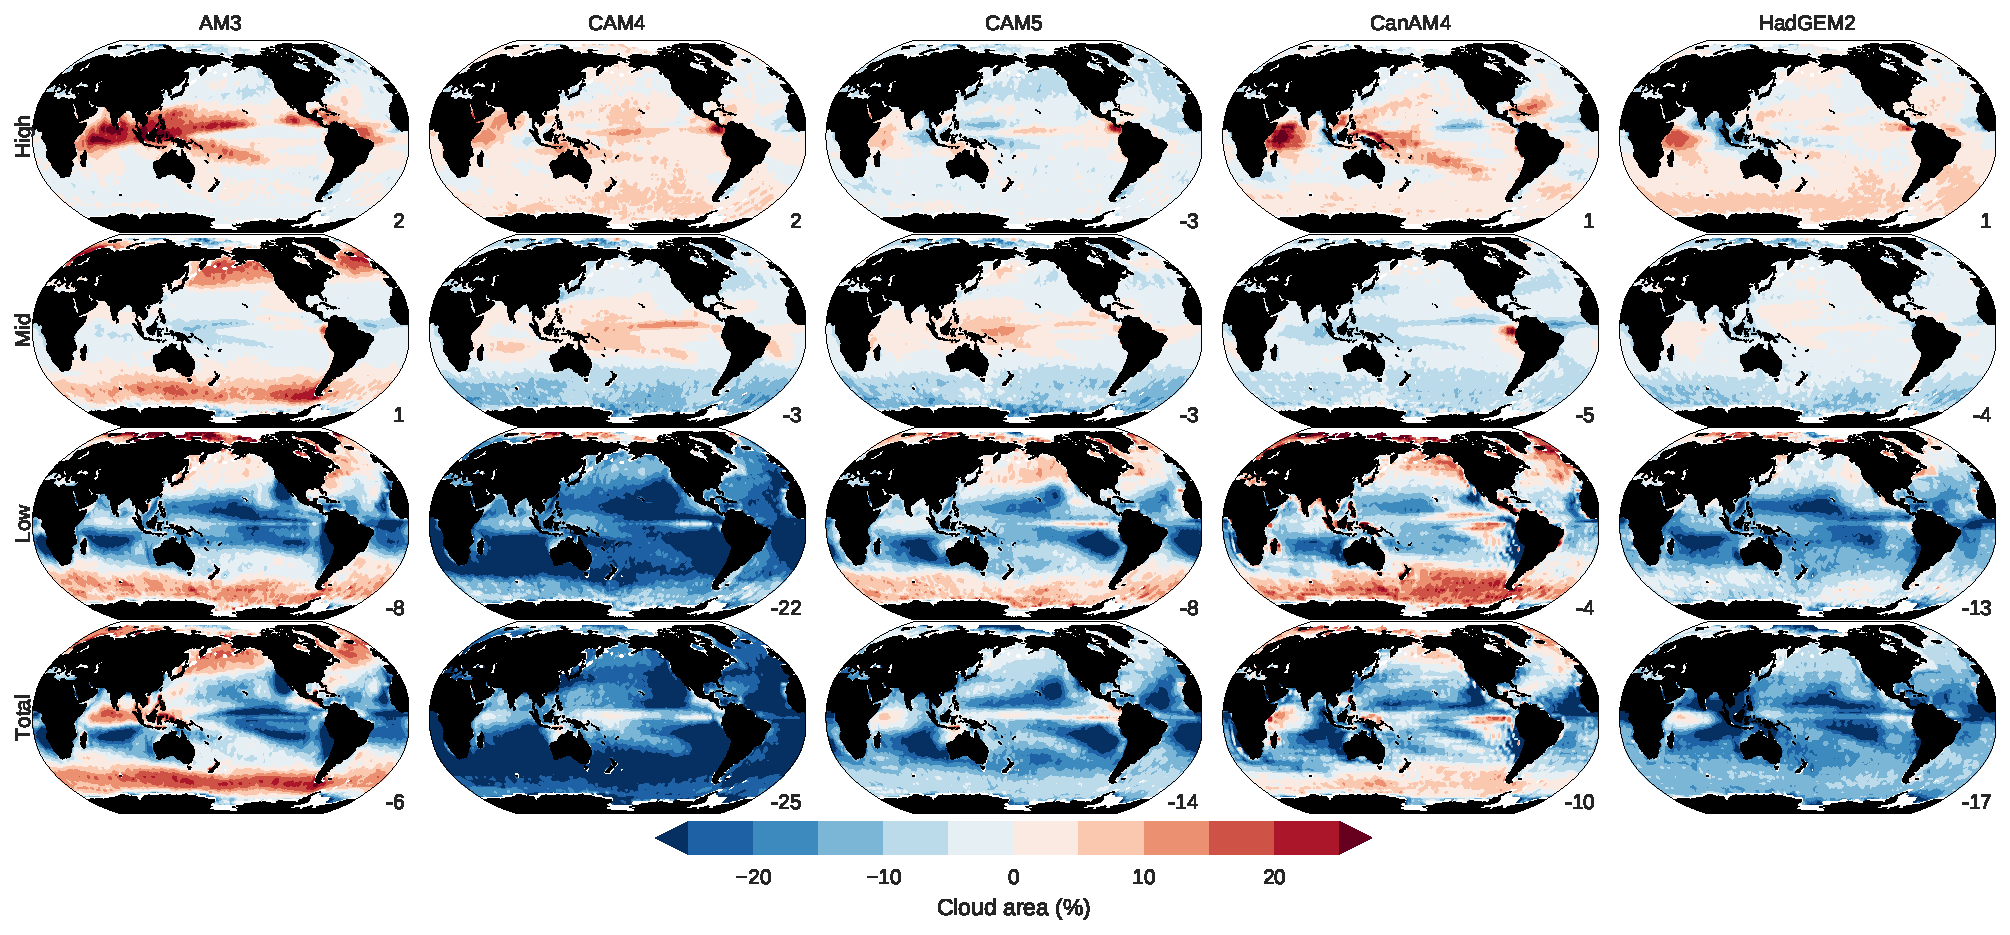
\includegraphics{graphics/cmip5_cldmisr_diff.pdf}
\caption{\label{fig:cmip5_cldmisr_maps_diff}Difference in MISR-simulated
total, high-topped, mid-topped, and low-topped cloud area in each of the
five models relative to MISR
retrievals.}\label{fig:cmip5ux5fcldmisrux5fmapsux5fdiff}
\end{figure}

\begin{figure}[htbp]
\centering
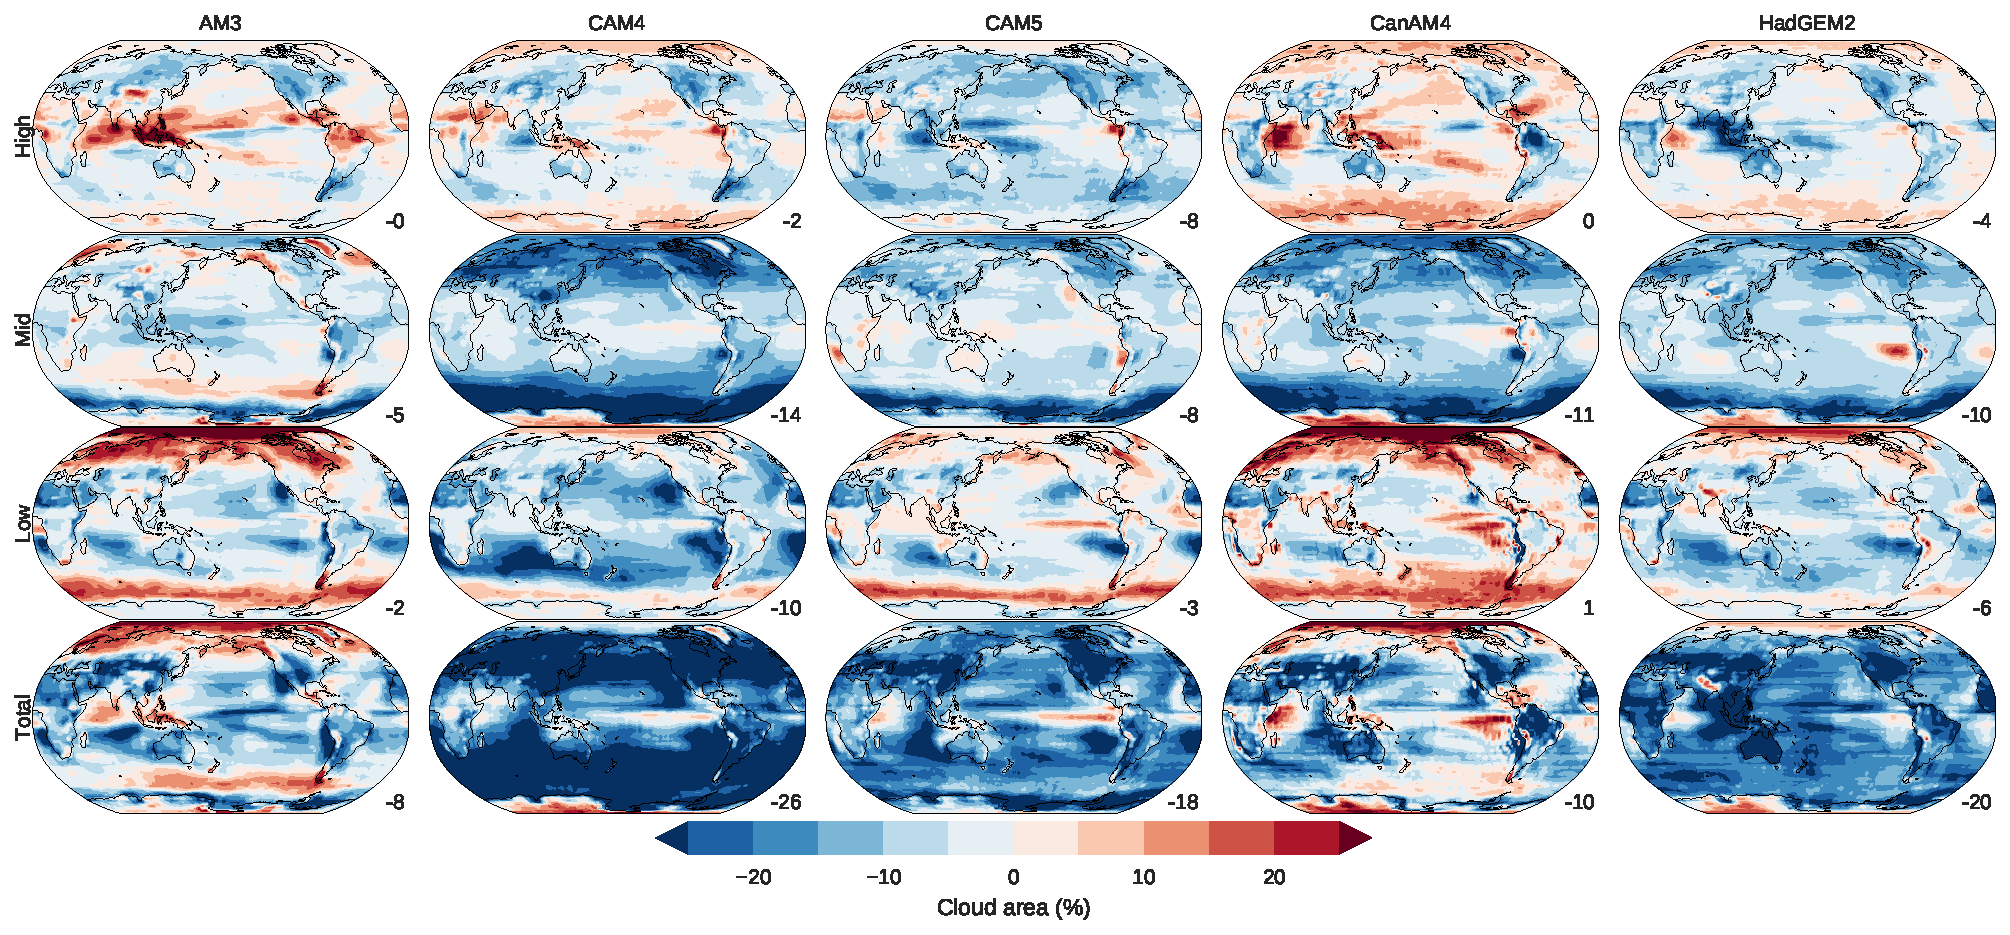
\includegraphics{graphics/cmip5_cldisccp_diff.pdf}
\caption{\label{fig:cmip5_cldisccp_maps_diff}Difference in
ISCCP-simulated total, high-topped, mid-topped, and low-topped cloud
area in each of the five models relative to ISCCP
retrievals.}\label{fig:cmip5ux5fcldisccpux5fmapsux5fdiff}
\end{figure}

Figure~\ref{fig:cmip5_cre_maps} shows shortwave and longwave cloud
radiative effects from CERES-EBAF and from each of the five models, and
Figure~\ref{fig:cmip5_cre_maps_diff} shows the differences between each
of the models and the CERES-EBAF observations. Indicated in each panel
of each figure are the global mean values. The global means agree well
between the CERES-EBAF observations and the models, with global mean
differences less than 5 W/m\(^2\) in all of the models. The patterns of
CRE are also similar in each of the models and the observations,
consistent with the well-known cloud regimes dominating different
regions of the globe. The differnce plots in
Figure~\ref{fig:cmip5_cre_maps_diff} show patterns of relative high
differences though throughout different regions. {[}comments on
differences specific to models\ldots{}lw vs sw{]}. These differences are
shown below to be traceable (using the simulator framework) to biases in
the simulated cloud statistics.

\begin{figure}[htbp]
\centering
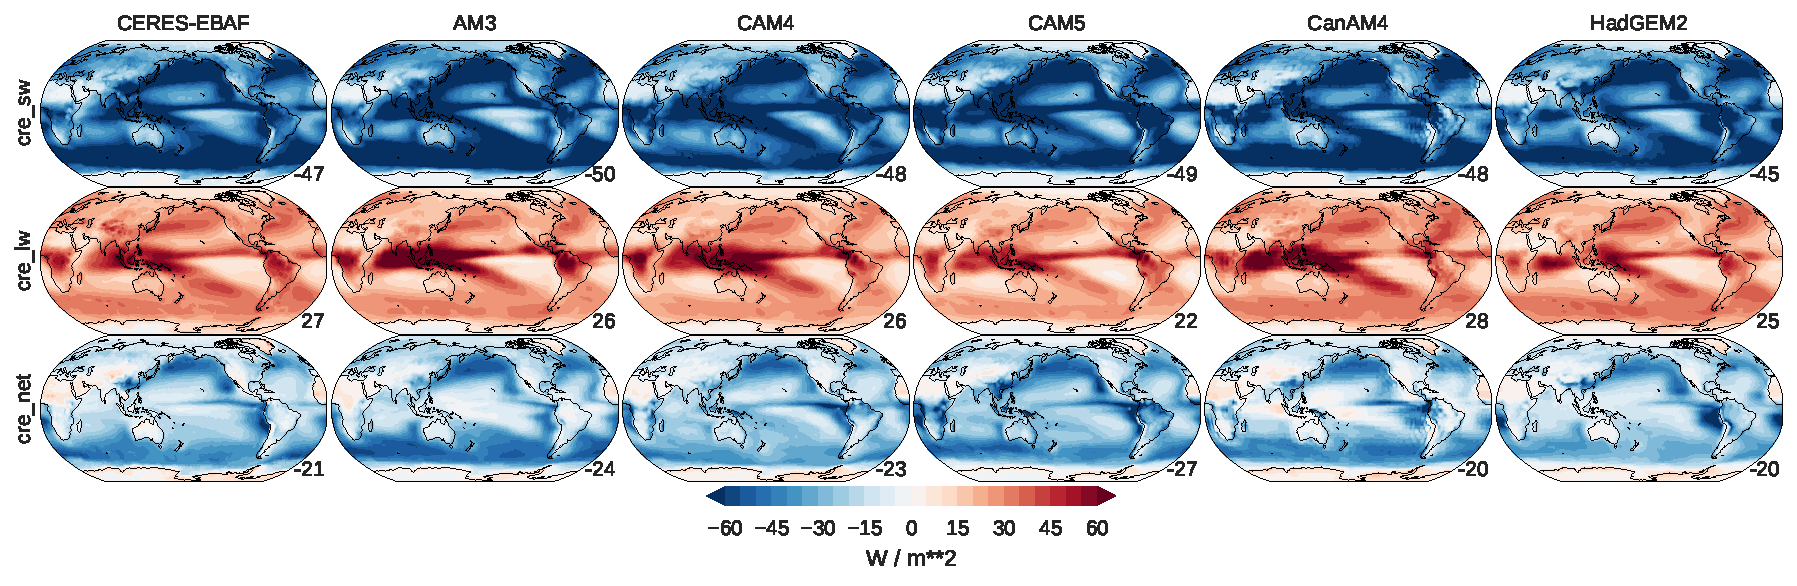
\includegraphics{graphics/cmip5_cre_maps.pdf}
\caption{\label{fig:cmip5_cre_maps}Shortwave (top), longwave (middle)
and net (bottom) cloud radiative effects from CERES-EBAF (left) and from
each of the five models evaluated in this study (from left to right,
AM3, CAM4, CAM5, CanAM4, HadGEM2). Numbers in the lower right corner of
each map indicate the area-weighted global
mean.}\label{fig:cmip5ux5fcreux5fmaps}
\end{figure}

\begin{figure}[htbp]
\centering
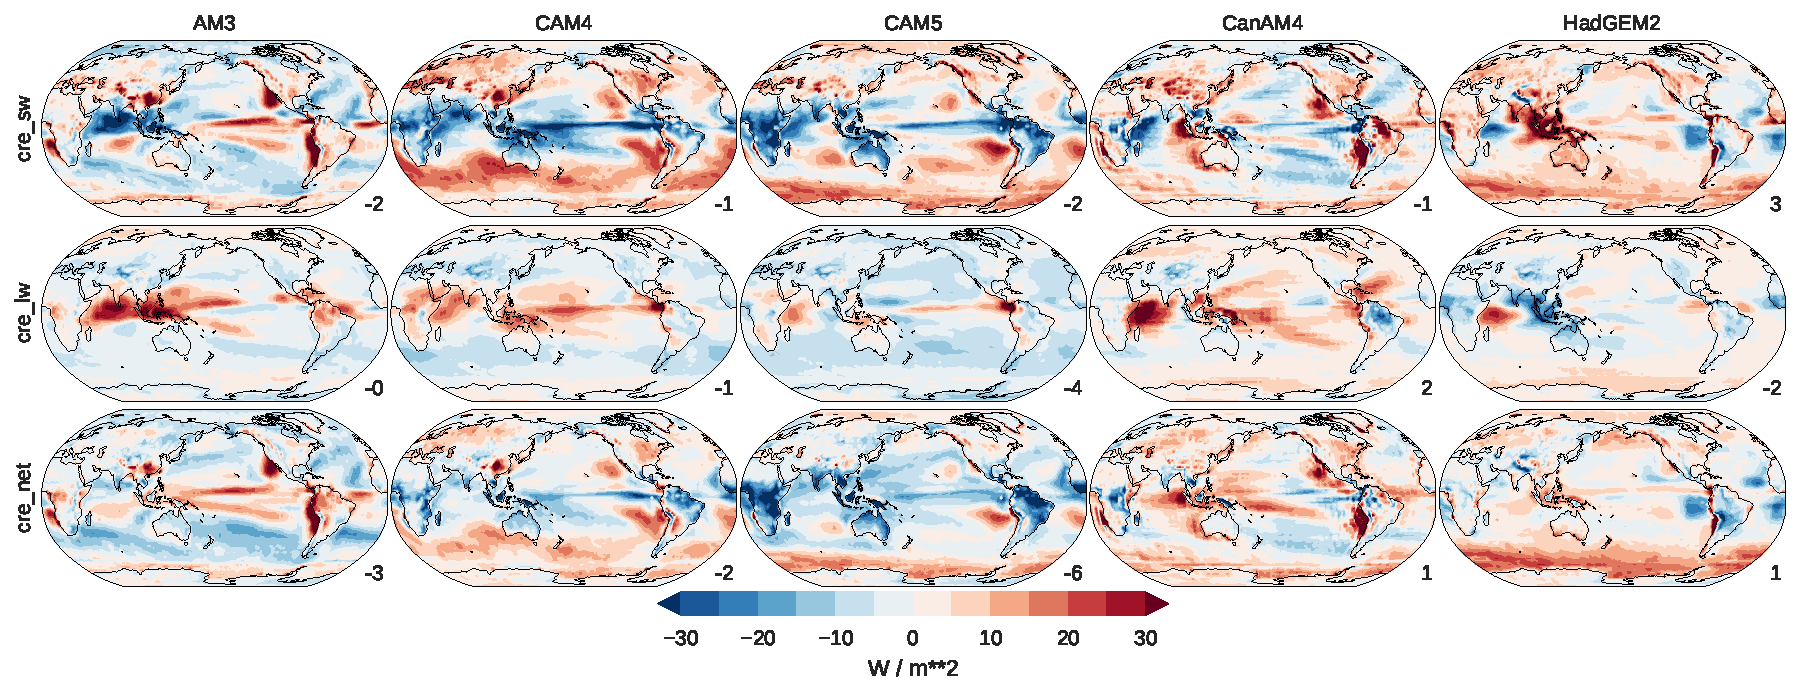
\includegraphics{graphics/cmip5_cre_maps_diff.pdf}
\caption{\label{fig:cmip5_cre_maps_diff}Differences in shortwave (top),
longwave (middle) and net (bottom) cloud radiative effects in each of
the five models relative to CERES-EBAF, calculated as model minus
observations. Numbers in the lower right corner of each map indicate the
area-weighted global mean of the
difference.}\label{fig:cmip5ux5fcreux5fmapsux5fdiff}
\end{figure}

Figure~\ref{fig:cmip5_cldmisr_maps_diff} and
Figure~\ref{fig:cmip5_cldisccp_maps_diff} show the differences between
MISR and ISCCP-simulated total, high-topped, mid-topped, and low-topped
cloud area in each of the models relative to the MISR and ISCCP
retrievals. These figures highlight differences in the simulated clouds
that are consistent with the differences in cloud radiative effects
identified in Figure~\ref{fig:cmip5_cre_maps_diff}. {[}comment on
specific differences\ldots{}what are the magnititudes? How do these
compare with the observational uncertainties idendified in
Section~\ref{sec:misr_chapter} and the expected errors identified in
Section~\ref{sec:subgrid1}? Also, calculate some kind of correlation
between the cloud area biases and the longwave and shortwave cloud
radiative effects\ldots{}differences tied to radiative effects? I expect
the errors to be correlated, and it would be a nice result to quantify
this\ldots{}{]}

\begin{figure}[htbp]
\centering
\includegraphics{graphics/cmip5_clMISR_TropicalWarmPool.pdf}
\caption{\label{fig:cmip5_clMISR_TropicalWarmPool}Joint histograms of
MISR-retrieved and MISR-simulated cloud top height and cloud optical
depth for the Tropical Warm
Pool.}\label{fig:cmip5ux5fclMISRux5fTropicalWarmPool}
\end{figure}

\begin{figure}[htbp]
\centering
\includegraphics{graphics/cmip5_clMISR_SouthernOcean.pdf}
\caption{\label{fig:cmip5_clMISR_SouthernOcean}Joint histograms of
MISR-retrieved and MISR-simulated cloud top height and cloud optical
depth for the Southern
Ocean.}\label{fig:cmip5ux5fclMISRux5fSouthernOcean}
\end{figure}

\section{Summary, discussion, and future
directions}\label{summary-discussion-and-future-directions}

This is the summary and discussion.

\hypertarget{refs}{}
\hypertarget{ref-ackermanux5fandux5fstokesux5f2003}{}
Ackerman, T. P., and G. M. Stokes. 2003. ``The Atmospheric Radiation
Measurement Program.'' \emph{Physics Today} 56: 38--44.

\hypertarget{ref-barkerux5f2008}{}
Barker, Howard W. 2008. ``Overlap of Fractional Cloud for Radiation
Calculations in GCMs: A Global Analysis Using CloudSat and CALIPSO
Data.'' \emph{J. Geophys. Res.} 113 (D00A01).
doi:\href{https://doi.org/10.1029/2007JD009677}{10.1029/2007JD009677}.

\hypertarget{ref-barkerux5fetux5falux5f1999}{}
Barker, Howard W., Graeme L. Stephens, and Qiang Fu. 1999. ``The
Sensitivity of Domain-Averaged Solar Fluxes to Assumptions About Cloud
Geometry.'' \emph{Q. J. R. Meteorol. Soc.} 125 (558): 2127--52.
doi:\href{https://doi.org/10.1256/smsqj.55809}{10.1256/smsqj.55809}.

\hypertarget{ref-berryux5fandux5fmaceux5f2014}{}
Berry, Elizabeth, and Gerald G Mace. 2014. ``Cloud Properties and
Radiative Effects of the Asian Summer Monsoon Derived from a-Train
Data.'' \emph{Journal of Geophysical Research: Atmospheres} 119 (15).
Wiley Online Library: 9492--9508.

\hypertarget{ref-bodas-salcedoux5fetux5falux5f2011}{}
Bodas-Salcedo, A., M. J. Webb, S. Bony, H. Chepfer, J.-L. Dufresne, S.
A. Klein, Y. Zhang, et al. 2011. ``COSP: Satellite Simulation Software
for Model Assessment.'' \emph{Bull. Amer. Meteor. Soc.} 92 (8).
doi:\href{https://doi.org/10.1175/2011BAMS2856.1}{10.1175/2011BAMS2856.1}.

\hypertarget{ref-bonyux5fandux5fdufresneux5f2005}{}
Bony, Sandrine, and Jean-Louis Dufresne. 2005. ``Marine Boundary Layer
Clouds at the Heart of Tropical Cloud Feedback Uncertainties in Climate
Models.'' \emph{Geophys. Res. Lett.} 32 (20).
doi:\href{https://doi.org/10.1029/2005GL023851}{10.1029/2005GL023851}.

\hypertarget{ref-bonyux5fetux5falux5f2006}{}
Bony, Sandrine, Robert Colman, Vladimir M. Kattsov, Richard P. Allan,
Christopher S. Bretherton, Jean-Louis Dufresne, Alex Hall, et al. 2006.
``How Well Do We Understand and Evaluate Climate Change Feedback
Processes?'' \emph{J. Climate} 19 (15): 3445--82.
doi:\href{https://doi.org/10.1175/JCLI3819.1}{10.1175/JCLI3819.1}.

\hypertarget{ref-brethertonux5fetux5falux5f2004}{}
Bretherton, Christopher S., Taneil Uttal, Christopher W. Fairall, Sandra
E. Yuter, Robert A. Weller, Darrel Baumgardner, Kimberly Comstock,
Robert Wood, and Graciela B. Raga. 2004. ``The EPIC 2001 Stratocumulus
Study.'' \emph{Bull. Amer. Meteor. Soc.} 85 (7): 967--77.
doi:\href{https://doi.org/10.1175/BAMS-85-7-967}{10.1175/BAMS-85-7-967}.

\hypertarget{ref-cahalanux5fetux5falux5f1994}{}
Cahalan, Robert F., William Ridgway, Warren J. Wiscombe, Thomas L. Bell,
and Jack B. Snider. 1994. ``The Albedo of Fractal Stratocumulus
Clouds.'' \emph{J. Atmos. Sci.} 51 (16): 2434--55.
doi:\href{https://doi.org/10.1175/1520-0469(1994)051$\%3C$2434:TAOFSC$\%3E$2.0.CO;2}{10.1175/1520-0469(1994)051\$\textless{}\$2434:TAOFSC\$\textgreater{}\$2.0.CO;2}.

\hypertarget{ref-cessux5fetux5falux5f1990}{}
Cess, R. D., G. L. Potter, J. P. Blanchet, G. J. Boer, A. D. Del Genio,
M. Déqué, V. Dymnikov, et al. 1990. ``Intercomparison and Interpretation
of Climate Feedback Processes in 19 Atmospheric General Circulation
Models.'' \emph{J. Geophys. Res.} 95 (D10): 16601--15.
doi:\href{https://doi.org/10.1029/JD095iD10p16601}{10.1029/JD095iD10p16601}.

\hypertarget{ref-chengux5fandux5fxuux5f2011}{}
Cheng, Anning, and Kuan-Man Xu. 2011. ``Improved Low-Cloud Simulation
from a Multiscale Modeling Framework with a Third-Order Turbulence
Closure in Its Cloud-Resolving Model Component.'' \emph{Journal of
Geophysical Research: Atmospheres} 116 (D14). Wiley Online Library.
doi:\href{https://doi.org/10.1029/2010JD015362}{10.1029/2010JD015362}.

\hypertarget{ref-chengux5fandux5fxuux5f2013}{}
---------. 2013. ``Evaluating Low-Cloud Simulation from an Upgraded
Multiscale Modeling Framework Model. Part III: Tropical and Subtropical
Cloud Transitions over the Northern Pacific.'' \emph{Journal of Climate}
26 (16): 5761--81.
doi:\href{https://doi.org/10.1175/JCLI-D-12-00650.1}{10.1175/JCLI-D-12-00650.1}.

\hypertarget{ref-chepferux5fetux5falux5f2008}{}
Chepfer, H., S. Bony, D. Winker, M. Chiriaco, J.-L. Dufresne, and G.
Sèze. 2008. ``Use of CALIPSO Lidar Observations to Evaluate the
Cloudiness Simulated by a Climate Model.'' \emph{Geophys. Res. Lett.} 35
(15).
doi:\href{https://doi.org/10.1029/2008GL034207}{10.1029/2008GL034207}.

\hypertarget{ref-collinsux5fetux5falux5f2004}{}
Collins, William D., Philip J. Rasch, Byron A. Boville, James J. Hack,
James R. McCaa, David L. Williamson, Jeffrey T. Kiehl, et al. 2004.
``Description of the NCAR Community Atmosphere Model (CAM 3.0).'' NCAR
Technical Note TN-464+STR. NCAR.

\hypertarget{ref-dengux5fetux5falux5f2013}{}
Deng, Min, Gerald G Mace, Zhien Wang, and R Paul Lawson. 2013.
``Evaluation of Several a-Train Ice Cloud Retrieval Products with in
Situ Measurements Collected During the SPARTICUS Campaign.''
\emph{Journal of Applied Meteorology and Climatology} 52 (4): 1014--30.

\hypertarget{ref-dengux5fetux5falux5f2010}{}
Deng, Min, Gerald G Mace, Zhien Wang, and Hajime Okamoto. 2010.
``Tropical Composition, Cloud and Climate Coupling Experiment Validation
for Cirrus Cloud Profiling Retrieval Using CloudSat Radar and CALIPSO
Lidar.'' \emph{Journal of Geophysical Research: Atmospheres} 115 (D10).
Wiley Online Library.

\hypertarget{ref-digirolamoux5fandux5fdaviesux5f1997}{}
Di Girolamo, Larry, and Roger Davies. 1997. ``Cloud Fraction Errors
Caused by Finite Resolution Measurements.'' \emph{Journal of Geophysical
Research: Atmospheres} 102 (D2). Wiley Online Library: 1739--56.
doi:\href{https://doi.org/10.1029/96JD02663}{10.1029/96JD02663}.

\hypertarget{ref-dimicheleux5fetux5falux5f2012}{}
Di Michele, Sabatino, Maike Ahlgrimm, Richard Forbes, Mark Kulie, Ralf
Bennartz Marta Janisková, and Peter Bauer. 2012. ``Interpreting an
Evaluation of the ECMWF Global Model with CloudSat Observations:
Ambiguities Due to Radar Reflectivity Forward Operator Uncertainties.''
\emph{Q. J. R. Meteorol. Soc.} 138: 2047--65.

\hypertarget{ref-dinerux5fetux5falux5f2002}{}
Diner, David J., Jewel C. Beckert, Graham W. Bothwell, and José I.
Rodriguez. 2002. ``Performance of the MISR Instrument During Its First
20 Months in Earth Orbit.'' \emph{IEEE Trans. Geosci. Remote Sens.} 40
(7): 1449--66.
doi:\href{https://doi.org/10.1109/TGRS.2002.801584}{10.1109/TGRS.2002.801584}.

\hypertarget{ref-dinerux5fetux5falux5f2005}{}
Diner, David J., Bobby H. Braswell, Roger Davies, Nadine Gobron, Jiannan
Hu, Yufang Jin, Ralph A. Kahn, et al. 2005. ``The Value of Multiangle
Measurements for Retrieving Structurally and Radiatively Consistent
Properties of Clouds, Aerosols, and Surfaces.'' \emph{Remote Sens.
Environ.} 97 (4): 495--518.
doi:\href{https://doi.org/10.1016/j.rse.2005.06.006}{10.1016/j.rse.2005.06.006}.

\hypertarget{ref-dongux5fandux5fmaceux5f2003}{}
Dong, Xiquan, and Gerald G Mace. 2003. ``Profiles of Low-Level Stratus
Cloud Microphysics Deduced from Ground-Based Measurements.''
\emph{Journal of Atmospheric and Oceanic Technology} 20 (1): 42--53.

\hypertarget{ref-donnerux5fetux5falux5f2011}{}
Donner, Leo J., Bruce L. Wyman, Richard S. Hemler, Larry W. Horowitz, Yi
Ming, Ming Zhao, Jean-Christophel Golaz, et al. 2011. ``The Dynamical
Core, Physical Parameterizations, and Basic Simulation Characteristics
of the Atmospheric Component AM3 of the GFDL Global Coupled Model CM3.''
\emph{J. Climate} 24 (13): 3484--3519.
doi:\href{https://doi.org/10.1175/2011JCLI3955.1}{10.1175/2011JCLI3955.1}.

\hypertarget{ref-dufresneux5fandux5fbonyux5f2008}{}
Dufresne, Jean-Louis, and Sandrine Bony. 2008. ``An Assessment of the
Primary Sources of Spread of Global Warming Estimates from Coupled
Atmosphere-Ocean Models.'' \emph{J. Climate} 21: 5135--44.
doi:\href{https://doi.org/10.1175/2008JCLI2239.1}{10.1175/2008JCLI2239.1}.

\hypertarget{ref-ellisux5fandux5fvonderhaarux5f1976}{}
Ellis, James S., and Thomas H. Vonder Haar. 1976. ``Zonal Average Earth
Radiation Budget Measurements from Satellites for Climate Studies.''
240. Dept. of Atmospheric Sciences, Colorado State University.

\hypertarget{ref-evansux5fetux5falux5f2008}{}
Evans, K Franklin, Alexander Marshak, and Tamás Várnai. 2008. ``The
Potential for Improved Boundary Layer Cloud Optical Depth Retrievals
from the Multiple Directions of MISR.'' \emph{Journal of the Atmospheric
Sciences} 65 (10): 3179--96.
doi:\href{https://doi.org/10.1175/2008JAS2627.1}{10.1175/2008JAS2627.1}.

\hypertarget{ref-flatoux5fetux5falux5f2013}{}
Flato, G, Jochem Marotzke, B Abiodun, P Braconnot, S Chan Chou, W
Collins, P Cox, et al. 2013. ``Evaluation of Climate Models.'' In
\emph{Climate Change 2013: The Physical Science Basis. Contribution of
Working Group I to the Fifth Assessment Report of the Intergovernmental
Panel on Climate Change}, 741--866. Cambridge University Press.

\hypertarget{ref-geleynux5fandux5fhollingsworthux5f1979}{}
Geleyn, J. F., and A. Hollingsworth. 1979. ``An Economical Analytical
Method for the Computation of the Interaction of Between Scattering and
Line Absorption of Radiation.'' \emph{Contrib. Atmos. Phys.} 52.

\hypertarget{ref-glecklerux5fetux5falux5f2008}{}
Gleckler, P. J., K. E. Taylor, and C. Doutriaux. 2008. ``Performance
Metrics for Climate Models.'' \emph{J. Geophys. Res.} 113 (D6).
doi:\href{https://doi.org/10.1029/2007JD008972}{10.1029/2007JD008972}.

\hypertarget{ref-golazux5fetux5falux5f2002}{}
Golaz, Jean-Christophe, Vincent E. Larson, and William R. Cotton. 2002.
``A PDF-Based Model for Boundary Layer Clouds. Part I: Method and Model
Description.'' \emph{J. Atmos. Sci.} 59 (24): 3540--51.
doi:\href{https://doi.org/10.1175/1520-0469(2002)059$\%3C$3540:APBMFB$\%3E$2.0.CO;2}{10.1175/1520-0469(2002)059\$\textless{}\$3540:APBMFB\$\textgreater{}\$2.0.CO;2}.

\hypertarget{ref-haynesux5fetux5falux5f2007}{}
Haynes, J. M., R. T. Marchand, Z. Luo, A. Bodas-Salcedo, and G. L.
Stephens. 2007. ``A Multipurpose Radar Simulation Package: Quickbeam.''
\emph{Bull. Amer. Meteor. Soc.} 88 (11): 1723--7.
doi:\href{https://doi.org/10.1175/BAMS-88-11-1723}{10.1175/BAMS-88-11-1723}.

\hypertarget{ref-hoganux5fandux5fillingworthux5f2000}{}
Hogan, Robin J., and Anthony J. Illingworth. 2000. ``Deriving Cloud
Overlap Statistics from Radar.'' \emph{Q. J. R. Meteorol. Soc.} 126:
2903--9.
doi:\href{https://doi.org/10.1256/smsqj.56913}{10.1256/smsqj.56913}.

\hypertarget{ref-hoganux5fetux5falux5f2014}{}
Hogan, Timothy F., Ming Liu, James A. Ridout, Melinda S. Peng, Timothy
R. Whitcomb, Benjamin C. Ruston, Carolyn A. Reynolds, et al. 2014. ``The
Navy Global Environmental Model.'' \emph{Oceanography} 27 (3).
doi:\href{https://doi.org/10.5670/oceanog.2014.73}{10.5670/oceanog.2014.73}.

\hypertarget{ref-iaconoux5fetux5falux5f2008}{}
Iacono, Michael J., Jennifer S. Delamere, Eli J. Mlawer, Mark W.
Shephard, Shepard A. Clough, and William D. Collins. 2008. ``Radiative
Forcing by Long-Lived Greenhouse Gases: Calculations with the AER
Radiative Transfer Models.'' \emph{J. Geophys. Res.} 113 (D13103).
doi:\href{https://doi.org/10.1029/2008JD009944}{10.1029/2008JD009944}.

\hypertarget{ref-kayux5fetux5falux5f2012}{}
Kay, J. E., B. R. Hillman, S. A. Klein, Y. Zhang, B. Medeiros, R.
Pincus, A. Gettelman, et al. 2012. ``Exposing Global Cloud Biases in the
Community Atmosphere Model (CAM) Using Satellite Observations and Their
Corresponding Instrument Simulators.'' \emph{J. Climate} 25: 5190--5207.
doi:\href{https://doi.org/\%7B10.1175/JCLI-D-11-00469.1\%7D}{\{10.1175/JCLI-D-11-00469.1\}}.

\hypertarget{ref-khairoutdinovux5fandux5frandallux5f2001}{}
Khairoutdinov, M. F., and D. A. Randall. 2001. ``A Cloud-Resolving Model
as a Cloud Parameterization in the NCAR Community Climate System Model:
Preliminary Results.'' \emph{Geophys. Res. Lett.} 28: 3617--20.

\hypertarget{ref-khairoutdinovux5fetux5falux5f2005}{}
Khairoutdinov, Marat, David Randall, and Charlotte DeMott. 2005.
``Simulations of the Atmospheric General Circulation Using a
Cloud-Resolving Model as a Superparameterization of Physical
Processes.'' \emph{Journal of the Atmospheric Sciences} 62 (7):
2136--54.
doi:\href{https://doi.org/10.1175/JAS3453.1}{10.1175/JAS3453.1}.

\hypertarget{ref-kingux5fetux5falux5f2013}{}
King, Michael D, Steven Platnick, W Paul Menzel, Steven A Ackerman, and
Paul A Hubanks. 2013. ``Spatial and Temporal Distribution of Clouds
Observed by MODIS Onboard the Terra and Aqua Satellites.''
\emph{Geoscience and Remote Sensing, IEEE Transactions on} 51 (7). IEEE:
3826--52.
doi:\href{https://doi.org/10.1109/TGRS.2012.2227333}{10.1109/TGRS.2012.2227333}.

\hypertarget{ref-kingux5fetux5falux5f2003}{}
King, Michael D., W. Paul Menzel, Yoram J. Kaufman, Didier Tanré, Bo-Cai
Gao, Steven Platnick, Steven A. Ackerman, Lorraine A. Remer, Robert
Pincus, and and Paul A. Hubanks. 2003. ``Cloud and Aerosol Properties,
Precipitable Water, and Profiles of Temperature and Water Vapor from
MODIS.'' \emph{IEEE Trans. Geosci. Remote Sens.} 41 (2): 442--58.
doi:\href{https://doi.org/10.1109/TGRS.2002.808226}{10.1109/TGRS.2002.808226}.

\hypertarget{ref-kleinux5fandux5fhartmannux5f1993}{}
Klein, Stephen A., and Dennis L. Hartmann. 1993. ``The Seasonal Cycle of
Low Stratiform Clouds.'' \emph{J. Climate} 6 (8): 1587--1606.
doi:\href{https://doi.org/10.1175/1520-0442(1993)006$\%3C$1587:TSCOLS$\%3E$2.0.CO;2}{10.1175/1520-0442(1993)006\$\textless{}\$1587:TSCOLS\$\textgreater{}\$2.0.CO;2}.

\hypertarget{ref-kleinux5fandux5fjakobux5f1999}{}
Klein, Stephen A., and Christian Jakob. 1999. ``Validation and
Sensitivities of Frontal Clouds Simulated by the ECMWF Model.''
\emph{Monthly Weather Review} 127 (10): 2514--31.
doi:\href{https://doi.org/10.1175/1520-0493(1999)127$\%3C$2514:VASOFC$\%3E$2.0.CO;2}{10.1175/1520-0493(1999)127\$\textless{}\$2514:VASOFC\$\textgreater{}\$2.0.CO;2}.

\hypertarget{ref-kleinux5fetux5falux5f2013}{}
Klein, Stephen A., Yuying Zhang, Mark D. Zelinka, Robert Pincus, James
Boyle, and Peter J. Gleckler. 2013. ``Are Climate Model Simulations of
Clouds Improving? An Evaluation Using the ISCCP Simulator.'' \emph{J.
Geophys. Res.} 118 (3): 1329--42.
doi:\href{https://doi.org/doi:10.1002/jgrd.50141}{doi:10.1002/jgrd.50141}.

\hypertarget{ref-leeux5fetux5falux5f2010}{}
Lee, Seungwon, Brian H. Kahn, and João Teixeira. 2010.
``Characterization of Cloud Liquid Water Content Distributions from
CloudSat.'' \emph{Journal of Geophysical Research: Atmospheres} 115
(D20).
doi:\href{https://doi.org/10.1029/2009JD013272}{10.1029/2009JD013272}.

\hypertarget{ref-wuux5fandux5fliangux5f2005}{}
Liang, Xiaoqing Wu And Xin-Zhong. 2005. ``Radiative Effects of Cloud
Horizontal Inhomogeneity and Vertical Overlap Identified from a
Monthlong Cloud-Resolving Model Simulation.'' \emph{J. Atmos. Sci.} 62:
4105--12.

\hypertarget{ref-linux5fandux5fzhangux5f2004}{}
Lin, W. Y., and M. H. Zhang. 2004. ``Evaluation of Clouds and Their
Radiative Effects Simulated by the NCAR Community Atmospheric Model
Against Satellite Observations.'' \emph{J. Climate} 17 (17): 3302--18.
doi:\href{https://doi.org/10.1175/1520-0442(2004)017$\%3C$3302:EOCATR$\%3E$2.0.CO;2}{10.1175/1520-0442(2004)017\$\textless{}\$3302:EOCATR\$\textgreater{}\$2.0.CO;2}.

\hypertarget{ref-loebux5fetux5falux5f2009}{}
Loeb, N. G., B. A. Wielicki, D. R. Doelling, G. L. Smith, D. F. Keyes,
S. Kato, N. Manalo-Smith, and T. Wong. 2009. ``Toward Optimal Closure of
the Earth's Top-of-Atmosphere Radiation Budget.'' \emph{J. Climate} 22
(3): 748--66.
doi:\href{https://doi.org/10.1175/2008JCLI2637.1}{10.1175/2008JCLI2637.1}.

\hypertarget{ref-maceux5f2010}{}
Mace, Gerald G. 2010. ``Cloud Properties and Radiative Forcing over the
Maritime Storm Tracks of the Southern Ocean and North Atlantic Derived
from a-Train.'' \emph{Journal of Geophysical Research: Atmospheres} 115
(D10). Wiley Online Library.

\hypertarget{ref-maceux5fandux5fzhangux5f2014}{}
Mace, Gerald G, and Qiuqing Zhang. 2014. ``The CloudSat Radar-Lidar
Geometrical Profile Product (RL-GeoProf): Updates, Improvements, and
Selected Results.'' \emph{Journal of Geophysical Research: Atmospheres}
119 (15). Wiley Online Library: 9441--62.

\hypertarget{ref-maceux5fetux5falux5f2006}{}
Mace, Gerald G, Sally Benson, Karen L Sonntag, Seiji Kato, Qilong Min,
Patrick Minnis, Cynthia H Twohy, et al. 2006. ``Cloud Radiative Forcing
at the Atmospheric Radiation Measurement Program Climate Research
Facility: 1. Technique, Validation, and Comparison to Satellite-Derived
Diagnostic Quantities.'' \emph{Journal of Geophysical Research:
Atmospheres} 111 (D11). Wiley Online Library.

\hypertarget{ref-maceux5fandux5fbenson-trothux5f2002}{}
Mace, Gerald G., and Sally Benson-Troth. 2002. ``Cloud-Layer Overlap
Characteristics Derived from Long-Term Cloud Radar Data.'' \emph{J.
Climate} 15.
doi:\href{https://doi.org/10.1175/1520-0442(2002)015$\%3C$2505:CLOCDF$\%3E$2.0.CO;2}{10.1175/1520-0442(2002)015\$\textless{}\$2505:CLOCDF\$\textgreater{}\$2.0.CO;2}.

\hypertarget{ref-maceux5fandux5fwrennux5f2013}{}
Mace, Gerald G., and Forrest J. Wrenn. 2013. ``Evaluation of the
Hydrometeor Layers in the East and West Pacific Within ISCCP Cloud-Top
Pressure-Optical Depth Bins USing Merged CloudSat and CALIPSO Data.''
\emph{J. Climate} 26: 9429--44.
doi:\href{https://doi.org/10.1175/JCLI-D-12-00207.1}{10.1175/JCLI-D-12-00207.1}.

\hypertarget{ref-maceux5fetux5falux5f2011}{}
Mace, Gerald G., Stephanie Houser, Sally Benson, Stephen A. Klein, and
Qilong Min. 2011. ``Critical Evaluation of the ISCCP Simulator Using
Ground-Based Remote Sensing Data.'' \emph{J. Climate} 24 (6):
1598--1612.
doi:\href{https://doi.org/10.1175/2010JCLI3517.1}{10.1175/2010JCLI3517.1}.

\hypertarget{ref-maceux5fetux5falux5f2009}{}
Mace, Gerald G., Qiuquing Zhang, Mark Vaughan, Roger Marchand, Graeme
Stephens, Chip Trepte, and Dave Winker. 2009. ``A Description of
Hydrometeor Layer Occurrence Statistics Derived from the First Year of
Merged Cloudsat and CALIPSO Data.'' \emph{J. Geophys. Res.} 114.
doi:\href{https://doi.org/10.1029/2007JD009755}{10.1029/2007JD009755}.

\hypertarget{ref-marchandux5fetux5falux5f2010}{}
Marchand, Roger, Thomas Ackerman, Mike Smyth, and William B. Rossow.
2010. ``A Review of Cloud Top Height and Optical Depth Histograms from
MISR, ISCCP and MODIS.'' \emph{J. Geophys. Res.} 115.
doi:\href{https://doi.org/10.1029/2009JD013422}{10.1029/2009JD013422}.

\hypertarget{ref-marchandux5fandux5fackermanux5f2010}{}
Marchand, Roger, and Thomas Ackerman. 2010. ``An Analysis of Cloud Cover
in Multiscale Modeling Framework Global Climate Model Simulations Using
4 and 1 Km Horizontal Grids.'' \emph{J. Geophys. Res.} 115.
doi:\href{https://doi.org/10.1029/2009JD013423}{10.1029/2009JD013423}.

\hypertarget{ref-marchandux5fetux5falux5f2009}{}
Marchand, Roger, John Haynes, Gerald G. Mace, and Thomas Ackerman. 2009.
``A Comparison of Simulated Radar Output from the Multiscale Modeling
Framework Global Climate Model with CloudSat Cloud Radar Observations.''
\emph{J. Geophys. Res.} 114.
doi:\href{https://doi.org/10.1029/2008JD009790}{10.1029/2008JD009790}.

\hypertarget{ref-medeirosux5fetux5falux5f2008}{}
Medeiros, Brian, Bjorn Stevens, Isaac M. Held, Ming Zhao, David L.
Williamson, Jerry G. Olson, and Christopher S. Bretherton. 2008.
``Aquaplanets, Climate Sensitivity, and Low Clouds.'' \emph{J. Climate}
21 (19): 4974--91.
doi:\href{https://doi.org/10.1175/2008JCLI1995.1}{10.1175/2008JCLI1995.1}.

\hypertarget{ref-meskhidzeux5fetux5falux5f2009}{}
Meskhidze, N, LA Remer, S Platnick, R Negrón Juárez, AM Lichtenberger,
and AR Aiyyer. 2009. ``Exploring the Differences in Cloud Properties
Observed by the Terra and Aqua MODIS Sensors.'' \emph{Atmospheric
Chemistry \& Physics Discussions} 9 (1).

\hypertarget{ref-morcretteux5fandux5ffouquartux5f1986}{}
Morcrette, Jean-Jacques, and Yves Fouquart. 1986. ``The Overlapping of
Cloud Layers in Shortwave Radiation Parameterizations.'' \emph{Journal
of the Atmospheric Sciences} 43 (4): 321--28.
doi:\href{https://doi.org/10.1175/1520-0469(1986)043\%3C0321:TOOCLI\%3E2.0.CO;2}{10.1175/1520-0469(1986)043\textless{}0321:TOOCLI\textgreater{}2.0.CO;2}.

\hypertarget{ref-moroneyux5fetux5falux5f2002}{}
Moroney, Catherine, Roger Davies, and Jan-Peter Muller. 2002.
``Operational Retrieval of Cloud-Top Heights Using MISR Data.''
\emph{IEEE Trans. Geosci. Remote Sens.} 40 (7): 1532--40.
doi:\href{https://doi.org/10.1109/TGRS.2002.801150}{10.1109/TGRS.2002.801150}.

\hypertarget{ref-mullerux5fetux5falux5f2002}{}
Muller, Jan-Peter, Athula Mandanayake, Catherine Moroney, Roger Davies,
David J. Diner, and Susan Paradise. 2002. ``MISR Stereoscopic Image
Matchers: Techniques and Results.'' \emph{IEEE Trans. Geosci. Remote
Sens.} 40 (7): 1547--59.
doi:\href{https://doi.org/10.1109/TGRS.2002.801160}{10.1109/TGRS.2002.801160}.

\hypertarget{ref-nealeux5fetux5falux5f2010b}{}
Neale, Richard B., Andrew Gettelman, Sungsu Park, Chih-Chieh Chen, Peter
H. Lauritzen, David L. Williamson, Andrew J. Conley, et al. 2010.
``Description of the NCAR Community Atmosphere Model (CAM 5.0).'' NCAR
Technical Note TN-486+STR. NCAR.

\hypertarget{ref-nealeux5fetux5falux5f2010a}{}
Neale, Richard B., Jadwiga H. Richter, Andrew J. Conley, Sungsu Park,
Peter H. Lauritzen, Andrew Gettelman, David L. Williamson, et al. 2010.
``Description of the NCAR Community Atmosphere Model (CAM 4.0).'' NCAR
Technical Note TN-485+STR. NCAR.

\hypertarget{ref-norrisux5fandux5fweaverux5f2001}{}
Norris, J. R., and C. P. Weaver. 2001. ``Improved Techniques for
Evaluating GCM Cloudiness Applied to the NCAR CCM3.'' \emph{J. Climate}
14 (12): 2540--50.
doi:\href{https://doi.org/10.1175/1520-0442(2001)014$\%3C$2540:ITFEGC$\%3E$2.0.CO;2}{10.1175/1520-0442(2001)014\$\textless{}\$2540:ITFEGC\$\textgreater{}\$2.0.CO;2}.

\hypertarget{ref-oreopoulosux5fetux5falux5f2012}{}
Oreopoulos, L., D. Lee, Y. C. Sud, and M. J. Suarez. 2012. ``Radiative
Impacts of Cloud Heterogeneity and Overlap in an Atmospheric General
Circulation Model.'' \emph{Atmos. Chem. Phys.} 12: 9097--9111.
doi:\href{https://doi.org/10.5194/acp-12-9097-2012}{10.5194/acp-12-9097-2012}.

\hypertarget{ref-pincusux5fetux5falux5f2012}{}
Pincus, R., S. Platnick, S. A. Ackerman, R. S. Hemler, and R. J. P.
Hofmann. 2012. ``Reconciling Simulated and Observed Views of Clouds:
MODIS, ISCCP, and and the Limits of Instrument Simulators.'' \emph{J.
Climate} 25: 4699--4720.
doi:\href{https://doi.org/10.1175/JCLI-D-11-00267.1}{10.1175/JCLI-D-11-00267.1}.

\hypertarget{ref-pincusux5fetux5falux5f2003}{}
Pincus, Robert, Howard W. Barker, and Jean-Jacques Morcrette. 2003. ``A
Fast, Flexible, Approximate Technique for Computing Radiative Transfer
in Inhomogeneous Cloud Fields.'' \emph{J. Geophys. Res.} 108 (D13).
doi:\href{https://doi.org/10.1029/2002JD003322}{10.1029/2002JD003322}.

\hypertarget{ref-pincusux5fetux5falux5f2005}{}
Pincus, Robert, Cécile Hannay, Stephen A. Klein, Kuan-Man Xu, and
Richard Hemler. 2005. ``Overlap Assumptions for Assumed Probability
Distribution Function Cloud Schemes in Large-Scale Models.'' \emph{J.
Geophys. Res.} 110 (D15S09).
doi:\href{https://doi.org/10.1029/2004JD005100}{10.1029/2004JD005100}.

\hypertarget{ref-ramanathanux5f1987}{}
Ramanathan, V. 1987. ``The Role of Earth Radiation Budget Studies in
Climate and General Circulation Research.'' \emph{J. Geophys. Res.} 92
(D4): 4075--95.
doi:\href{https://doi.org/10.1029/JD092iD04p04075}{10.1029/JD092iD04p04075}.

\hypertarget{ref-ramanathanux5fetux5falux5f1989}{}
Ramanathan, V., R. D. Cess, E. F. Harrison, P. Minnis, B. R. Barkstrom,
E. Ahmad, and D. Hartmann. 1989. ``Cloud-Radiative Forcing and Climate:
Results from the Earth Radiation Budget Experiment.'' \emph{Science} 243
(4887): 57--63.
doi:\href{https://doi.org/10.1126/science.243.4887.57}{10.1126/science.243.4887.57}.

\hypertarget{ref-randallux5fetux5falux5f2003}{}
Randall, David, Marat Khairoutdinov, Akio Arakawa, and Wojciech
Grabowski. 2003. ``Breaking the Cloud Parameterization Deadlock.''
\emph{Bull. Amer. Meteor. Soc.} 84 (11): 1547--64.
doi:\href{https://doi.org/10.1175/BAMS-84-11-1547}{10.1175/BAMS-84-11-1547}.

\hypertarget{ref-raisanenux5fetux5falux5f2004}{}
Räisänen, Petri, Howard W. Barker, Marat F. Khairoutdinov, Jiangnan Li,
and David A. Randall. 2004. ``Stochastic Generation of Subgrid-Scale
Cloudy Columns for Large-Scale Models.'' \emph{Q. J. R. Meteorol. Soc.}
130: 2047--67.
doi:\href{https://doi.org/10.1256/qj.03.99}{10.1256/qj.03.99}.

\hypertarget{ref-rossowux5fandux5fschifferux5f1999}{}
Rossow, W. B., and R. A. Schiffer. 1999. ``Advances in Understanding
Clouds from ISCCP.'' \emph{Bull. Amer. Meteor. Soc.} 80 (11): 2261--87.
doi:\href{https://doi.org/10.1175/1520-0477(1999)080$\%3C$2261:AIUCFI$\%3E$2.0.CO;2}{10.1175/1520-0477(1999)080\$\textless{}\$2261:AIUCFI\$\textgreater{}\$2.0.CO;2}.

\hypertarget{ref-vonux5fsalzenux5fetux5falux5f2012}{}
Salzen, Knut von, John Scinocca, Norman McFarlane, Jiangnan Li, Jason
Cole, David Plummer, Cathy Reader, Xiaoyan Ma, Michael Lazare, and Larry
Solheim. 2012. ``The Canadian Fourth Generation Atmospheric Global
Climate Model (CanAM4): Simulation of Clouds and Precipitation and Their
Responses to Short-Term Climate Variability.'' \emph{Atmos.-Ocean}.

\hypertarget{ref-stephensux5f2005}{}
Stephens, Graeme L. 2005. ``Cloud Feedbacks in the Climate System: A
Critical Review.'' \emph{J. Climate} 18 (2): 237--73.
doi:\href{https://doi.org/10.1175/JCLI-3243.1}{10.1175/JCLI-3243.1}.

\hypertarget{ref-stephensux5fandux5fplattux5f1987}{}
Stephens, Graeme L., and C. M. R. Platt. 1987. ``Aircraft Observations
of the Radiative and Microphysical Properties of Stratocumulus and
Cumulus Cloud Fields.'' \emph{J. Climate Appl. Meteor.} 26: 1243--69.
doi:\href{https://doi.org/10.1175/1520-0450(1987)026$\%3C$1243:AOOTRA$\%3E$2.0.CO;2}{10.1175/1520-0450(1987)026\$\textless{}\$1243:AOOTRA\$\textgreater{}\$2.0.CO;2}.

\hypertarget{ref-stephensux5fetux5falux5f2002}{}
Stephens, Graeme L., Deborah G. Vane, Ronald J. Boain, Gerald G. Mace,
Kenneth Sassen, Zhien Wang, Anthony J. Illingworth, et al. 2002. ``The
CloudSat Mission and the A-Train.'' \emph{Bull. Amer. Meteorol. Soc.} 83
(12): 1771--90.
doi:\href{https://doi.org/10.1175/BAMS-83-12-1771}{10.1175/BAMS-83-12-1771}.

\hypertarget{ref-stubenrauchux5fetux5falux5f1997}{}
Stubenrauch, C. J., A. D. Del Genio, and W. B. Rossow. 1997.
``Implementation of Subgrid Cloud Vertical Structure Inside a GCM and
Its Effect on the Radiation Budget.'' \emph{J. Climate.} 10: 273--87.

\hypertarget{ref-tanelliux5fetux5falux5f2008}{}
Tanelli, Simone, Stephen L Durden, Eastwood Im, Kyung S Pak, Dale G
Reinke, Philip Partain, John M Haynes, and Roger T Marchand. 2008.
``CloudSat's Cloud Profiling Radar After Two Years in Orbit:
Performance, Calibration, and Processing.'' \emph{Geoscience and Remote
Sensing, IEEE Transactions on} 46 (11). IEEE: 3560--73.
doi:\href{https://doi.org/10.1109/TGRS.2008.2002030}{10.1109/TGRS.2008.2002030}.

\hypertarget{ref-taoux5fetux5falux5f2009}{}
Tao, Wei-Kuo, Jiun-Dar Chern, Robert Atlas, David Randall, Marat
Khairoutdinov, Jui-Lin Li, Duane E Waliser, et al. 2009. ``A Multiscale
Modeling System: Developments, Applications, and Critical Issues.''
\emph{Bulletin of the American Meteorological Society} 90 (4). American
Meteorological Society: 515.

\hypertarget{ref-martinux5fetux5falux5f2011}{}
The HadGEM2 Development Team: Martin, G. M., N. Bellouin, W. J. Collins,
I. D. Culverwell, P. R. Halloran, S. C. Hardiman, T. J. Hinton, et al.
2011. ``The HadGEM2 Family of Met Office Unified Model Climate
Configurations.'' \emph{Geoscientific Model Development} 4 (3): 723--57.
doi:\href{https://doi.org/10.5194/gmd-4-723-2011}{10.5194/gmd-4-723-2011}.

\hypertarget{ref-tianux5fandux5fcurryux5f1989}{}
Tian, Lin, and Judith A. Curry. 1989. ``Cloud Overlap Statistics.''
\emph{J. Geophys. Res.} 94 (D7): 9925--35.

\hypertarget{ref-tompkinsux5fandux5fdigiuseppeux5f2015}{}
Tompkins, Adrian M, and Francesca Di Giuseppe. 2015. ``An Interpretation
of Cloud Overlap Statistics.'' \emph{Journal of the Atmospheric
Sciences} 72 (8): 2877--89.

\hypertarget{ref-tompkinsux5f2002}{}
Tompkins, Adrian. M. 2002. ``A Prognostic Parameterization for the
Subgrid-Scale Variability of Water Vapor and Clouds in Large-Scale
Models and Its Use to Diagnose Cloud Cover.'' \emph{J. Atmos. Sci.} 59:
1917--42.
doi:\href{https://doi.org/10.1175/1520-0469(2002)059$\%3C$1917:APPFTS$\%3E$2.0.CO;2}{10.1175/1520-0469(2002)059\$\textless{}\$1917:APPFTS\$\textgreater{}\$2.0.CO;2}.

\hypertarget{ref-warrenux5fetux5falux5f1986}{}
Warren, Stephen G, Carole J Hahn, Julius London, Robert M Chervin, and
Roy L Jenne. 1986. ``Global Distribution of Total Cloud Cover and Cloud
Type Amounts over Land.'' Washington Univ., Seattle (USA). Dept. of
Atmospheric Sciences; Colorado Univ., Boulder (USA); National Center for
Atmospheric Research, Boulder, CO (USA).

\hypertarget{ref-warrenux5fetux5falux5f1988}{}
---------. 1988. ``Global Distribution of Total Cloud Cover and Cloud
Type Amounts over the Ocean.'' USDOE Office of Energy Research,
Washington, DC (USA). Carbon Dioxide Research Div.; National Center for
Atmospheric Research, Boulder, CO (USA).

\hypertarget{ref-webbux5fetux5falux5f2001}{}
Webb, M., C. Senior, S. Bony, and J.-J. Morcrette. 2001. ``Combining
ERBE and ISCCP Data to Assess Clouds in the Hadley Centre, ECMWF and LMD
Atmospheric Climate Models.'' \emph{Clim. Dyn.} 17 (12): 905--22.
doi:\href{https://doi.org/10.1007/s003820100157}{10.1007/s003820100157}.

\hypertarget{ref-wielickiux5fandux5fparkerux5f1992}{}
Wielicki, Bruce A, and Lindsay Parker. 1992. ``On the Determination of
Cloud Cover from Satellite Sensors: The Effect of Sensor Spatial
Resolution.'' \emph{Journal of Geophysical Research: Atmospheres} 97
(D12). Wiley Online Library: 12799--12823.
doi:\href{https://doi.org/10.1029/92JD01061}{10.1029/92JD01061}.

\hypertarget{ref-wilksux5f2011}{}
Wilks, Daniel S. 2011. \emph{Statistical Methods in the Atmospheric
Sciences}. Vol. 100. Academic press.

\hypertarget{ref-williamsux5fandux5fwebbux5f2009}{}
Williams, K. D., and M. J. Webb. 2009. ``A Quantitative Performance
Assessment of Cloud Regimes in Climate Models.'' \emph{Clim. Dyn.} 33
(1): 141--57.
doi:\href{https://doi.org/10.1007/s00382-008-0443-1}{10.1007/s00382-008-0443-1}.

\hypertarget{ref-winkerux5fetux5falux5f2007}{}
Winker, D. M., B. H. Hunt, and M. J. McGill. 2007. ``Initial Performance
Assessment of CALIOP.'' \emph{Geophys. Res. Lett.} 34 (L19803).
doi:\href{https://doi.org/10.1029/2007GL030135}{10.1029/2007GL030135}.

\hypertarget{ref-wyantux5fetux5falux5f2006}{}
Wyant, Matthew C, Christopher S Bretherton, Julio T Bacmeister, Jeffrey
T Kiehl, Isaac M Held, Ming Zhao, Stephen A Klein, and Brian J Soden.
2006. ``A Comparison of Low-Latitude Cloud Properties and Their Response
to Climate Change in Three AGCMs Sorted into Regimes Using
Mid-Tropospheric Vertical Velocity.'' \emph{Climate Dynamics} 27 (2-3).
Springer: 261--79.

\hypertarget{ref-yangux5fandux5fdigirolamoux5f2008}{}
Yang, Yuekui, and Larry Di Girolamo. 2008. ``Impacts of 3-d Radiative
Effects on Satellite Cloud Detection and Their Consequences on Cloud
Fraction and Aerosol Optical Depth Retrievals.'' \emph{Journal of
Geophysical Research: Atmospheres} 113 (D4). Wiley Online Library.
doi:\href{https://doi.org/10.1029/2007JD009095}{10.1029/2007JD009095}.

\hypertarget{ref-zelinkaux5fetux5falux5f2012a}{}
Zelinka, Mark D, Stephen A Klein, and Dennis L Hartmann. 2012a.
``Computing and Partitioning Cloud Feedbacks Using Cloud Property
Histograms. Part I: Cloud Radiative Kernels.'' \emph{Journal of Climate}
25 (11): 3715--35.
doi:\href{https://doi.org/10.1175/JCLI-D-11-00248.1}{10.1175/JCLI-D-11-00248.1}.

\hypertarget{ref-zelinkaux5fetux5falux5f2012b}{}
---------. 2012b. ``Computing and Partitioning Cloud Feedbacks Using
Cloud Property Histograms. Part II: Attribution to Changes in Cloud
Amount, Altitude, and Optical Depth.'' \emph{Journal of Climate} 25
(11): 3736--54.
doi:\href{https://doi.org/10.1175/JCLI-D-11-00249.1}{10.1175/JCLI-D-11-00249.1}.

\hypertarget{ref-zhangux5fetux5falux5f2005}{}
Zhang, M.H., W. Y. Lin, S. A. Klein, J. T. Bacmeister, S. Bony, R. T.
Cederwall, A. D. Del Genio, et al. 2005. ``Comparing Clouds and Their
Seasonal Variations in 10 Atmospheric General Circulation Models with
Satellite Measurements.'' \emph{J. Geophys. Res.} 110 (D15).
doi:\href{https://doi.org/10.1029/2004JD005021}{10.1029/2004JD005021}.

\hypertarget{ref-zhangux5fetux5falux5f2010}{}
Zhang, Y., S. A. Klein, J. Boyle, and G. G. Mace. 2010. ``Evaluation of
Tropical Cloud and Precipitation Statistics of Community Atmosphere
Model Version 3 Using CloudSat and CALIPSO Data.'' \emph{J. Geophys.
Res.} 115 (D12205).
doi:\href{https://doi.org/10.1029/2009JD012006}{10.1029/2009JD012006}.

\hypertarget{ref-zhaoux5fandux5fdigirolamoux5f2006}{}
Zhao, Guangyu, and Larry Di Girolamo. 2006. ``Cloud Fraction Errors for
Trade Wind Cumuli from EOS-Terra Instruments.'' \emph{Geophysical
Research Letters} 33 (20). Wiley Online Library.
